%\documentclass[12pt,a4paper]{scrartcl}
\documentclass[12pt,a4paper]{book}

\makeatletter % Technical doc - START

\usepackage[utf8]{inputenc}
\usepackage[T1]{fontenc}
\usepackage{ucs}

\usepackage[french]{babel,varioref}

\usepackage[top=2cm, bottom=2cm, left=1.5cm, right=1.5cm]{geometry}
\usepackage{enumitem}

\usepackage{multicol}

\usepackage{makecell}

\usepackage{color}
\usepackage{hyperref}
\hypersetup{
    colorlinks,
    citecolor=black,
    filecolor=black,
    linkcolor=black,
    urlcolor=black
}

\usepackage{amsthm}

\usepackage{tcolorbox}
\tcbuselibrary{listingsutf8}

\usepackage{ifplatform}

\usepackage{ifthen}

\usepackage{macroenvsign}


% Sections numbering

\renewcommand\thechapter{\Roman{chapter}.}
\renewcommand\thesection{\arabic{section}.}
\renewcommand\thesubsection{\alph{subsection}.}
\renewcommand\thesubsubsection{\roman{subsubsection}.}

\setcounter{tocdepth}{3}
\setcounter{secnumdepth}{3}


% MISC

\newtcblisting{latexex}{%
	sharp corners,%
	left=1mm, right=1mm,%
	bottom=1mm, top=1mm,%
	colupper=red!75!blue,%
	listing side text
}

\newtcbinputlisting{\inputlatexex}[2][]{%
	listing file={#2},%
	sharp corners,%
	left=1mm, right=1mm,%
	bottom=1mm, top=1mm,%
	colupper=red!75!blue,%
	listing side text
}


\newtcblisting{latexex-flat}{%
	sharp corners,%
	left=1mm, right=1mm,%
	bottom=1mm, top=1mm,%
	colupper=red!75!blue,%
}

\newtcbinputlisting{\inputlatexexflat}[2][]{%
	listing file={#2},%
	sharp corners,%
	left=1mm, right=1mm,%
	bottom=1mm, top=1mm,%
	colupper=red!75!blue,%
}


\newtcblisting{latexex-alone}{%
	sharp corners,%
	left=1mm, right=1mm,%
	bottom=1mm, top=1mm,%
	colupper=red!75!blue,%
	listing only
}

\newtcbinputlisting{\inputlatexexalone}[2][]{%
	listing file={#2},%
	sharp corners,%
	left=1mm, right=1mm,%
	bottom=1mm, top=1mm,%
	colupper=red!75!blue,%
	listing only
}


\newcommand\inputlatexexcodeafter[1]{%
	\begin{center}
		\input{#1}
	\end{center}

	\vspace{-.5em}
	
	Le rendu précédent a été obtenu via le code suivant.
	
	\inputlatexexalone{#1}
}


\newcommand\inputlatexexcodebefore[1]{%
	\inputlatexexalone{#1}
	\vspace{-.75em}
	\begin{center}
		\textit{\footnotesize Rendu du code précédent}
		
		\medskip
		
		\input{#1}
	\end{center}
}


\newcommand\env[1]{\texttt{#1}}
\newcommand\macro[1]{\env{\textbackslash{}#1}}



\setlength{\parindent}{0cm}
\setlist{noitemsep}

\theoremstyle{definition}
\newtheorem*{remark}{Remarque}

\usepackage[raggedright]{titlesec}

\titleformat{\paragraph}[hang]{\normalfont\normalsize\bfseries}{\theparagraph}{1em}{}
\titlespacing*{\paragraph}{0pt}{3.25ex plus 1ex minus .2ex}{0.5em}


\newcommand\separation{
	\medskip
	\hfill\rule{0.5\textwidth}{0.75pt}\hfill
	\medskip
}


\newcommand\extraspace{
	\vspace{0.25em}
}


\newcommand\whyprefix[2]{%
	\textbf{\prefix{#1}}-#2%
}

\newcommand\mwhyprefix[2]{%
	\texttt{#1 = #1-#2}%
}

\newcommand\prefix[1]{%
	\texttt{#1}%
}


\newcommand\inenglish{\@ifstar{\@inenglish@star}{\@inenglish@no@star}}

\newcommand\@inenglish@star[1]{%
	\emph{\og #1 \fg}%
}

\newcommand\@inenglish@no@star[1]{%
	\@inenglish@star{#1} en anglais%
}


\newcommand\ascii{\texttt{ASCII}}


% Example
\newcounter{paraexample}[subsubsection]

\newcommand\@newexample@abstract[2]{%
	\paragraph{%
		#1%
		\if\relax\detokenize{#2}\relax\else {} -- #2\fi%
	}%
}



\newcommand\newparaexample{\@ifstar{\@newparaexample@star}{\@newparaexample@no@star}}

\newcommand\@newparaexample@no@star[1]{%
	\refstepcounter{paraexample}%
	\@newexample@abstract{Exemple \theparaexample}{#1}%
}

\newcommand\@newparaexample@star[1]{%
	\@newexample@abstract{Exemple}{#1}%
}


% Change log
\newcommand\topic{\@ifstar{\@topic@star}{\@topic@no@star}}

\newcommand\@topic@no@star[1]{%
	\textbf{\textsc{#1}.}%
}

\newcommand\@topic@star[1]{%
	\textbf{\textsc{#1} :}%
}

\makeatother % Technical doc - END


\usepackage{tnsmath}


\begin{document}

\renewcommand\labelitemi{\raisebox{0.125em}{\tiny\textbullet}}
\renewcommand{\labelitemii}{---}

\title{%
	Le package \texttt{tnsmath}:\\%
	des formules plus sémantiques\\%
	{\footnotesize Code source disponible sur \url{https://github.com/typensee-latex/tnsmath.git}.}\\%
{\footnotesize Version \texttt{1.5.0-beta} développée et testée sur \macosxname{}.}%
}
\author{Christophe BAL}
\date{2020-07-23}{{

\maketitle


\vspace{2em}

\hrule

\tableofcontents


\chapter{Généralités}

\section{Introduction}

\LaTeX{} est un excellent langage, pour ne pas dire le meilleur, pour rédiger des documents contenant des formules mathématiques.
Malheureusement toute la puissance de \LaTeX{} permet d'écrire des codes très peu sémantiques.
Le modeste but du package \verb+tnsmath+ est de fournir quelques macros sémantiques
\footnote{
	En fait l'aspect sémantique est l'objectif commun de tous les packages de la suite \texttt{tns}.
}
pour la rédaction de documents mathématiques élémentaires. Considérons le code \LaTeX{} suivant.

\begin{latexex-alone}
Sachant que $f^\prime(x) = cos(x^2)$ sur $[a ; b]$ , nous avons :

$\displaystyle \int_a^b cos(x^2) dx = \left[ f(x) \right]_{x=a}^{x=b}$.
\end{latexex-alone}


Avec \verb+tnsmath+, vous pouvez écrire le code suivant.

\begin{latexex-alone}
Sachant que $\sder{f}(x) = cos(x^2)$ sur $\intervalC{a}{b}$, nous avons :

$\dintegrate*{a}{b}{cos(x^2)}{x} = \hook{a}{b}{f(x)}{x}$.
\end{latexex-alone}


Même si certaines commandes sont plus longues à écrire que ce que permet \LaTeX{}, il y a des avantages à utiliser des commandes sémantiques.
\begin{enumerate}
	\item La mise en forme du document devient consistante.

	\item Il est facile de changer une mise en forme sur l'ensemble d'un document ou localement via certaines options.

	\item \verb+tnsmath+ résout certains problèmes \og complexes \fg{} pour vous.
\end{enumerate}


% ---------------------- %


\section{Béta-dépendance}

Ce package dépend de \verb+tnscom+
\footnote{
	Lui est aussi en version \texttt{beta}.
}
disponible sur \url{https://github.com/typensee-latex/tnscom.git} pour une installation locale.
\section{Comment lire cette documentation ?}

Le choix a été fait de fournir des exemples comme documentation du package et de donner des fiches techniques des macros-commandes dans le chapitre dédié \ref{techincal-ids}.
Les exemples se présentent comme ci-dessous et sont généralement très courts.

\begin{latexex}
$\dintegrate*{a}{b}{cos(x^2)}{x}
 =
 \hook*{a}{b}{f(x)}{x}$
\end{latexex}
\section{A propos des macros}

\subsection{Règles de nommage}

\subsubsection{Les macros de même \og type \fg}

Les macros partageant une même fonctionnalité mathématique suivent les règles suivantes.

\begin{enumerate}[itemsep = .5em]
	\item Un nom de base explicite est choisi comme par exemple \prefix{dotproduct} pour \inenglish{produit scalaire} ou \prefix{set} pour \inenglish{ensemble}.

	\item Si besoin on spécialise du point de vue sémantique avec un préfixe et/ou un suffixe. Voici deux exemples.
	\begin{enumerate}
		\item Dans \macro{vdotproduct}, le préfixe \prefix{v} est pour \whyprefix{v}{ecteur} car cette macro s'utilise avec des noms de vecteurs \verb+u+ et \verb+v+ et non directement des vecteurs \verb+\vect{u}+ et \verb+\vect{v}+, autrement dit c'est \macro{vdotproduct} qui se charge d'appliquer \verb+\vect+ à \verb+u+ et \verb+v+.

		\item Dans \macro{setproba}, le suffixe \prefix{proba} est pour \whyprefix{proba}{bilité} car cette macro sert à écrire des ensembles munis d'une probabilité
	      \footnote{
	      	Ce choix est assumé même si on obtient un nom faisant penser à \emph{\og régler ... \fg} au lieu de \emph{\og ensemble de type ... \fg}.
		  }.
	\end{enumerate}

	\item Si l'on propose différentes mises en forme pour une même signification sémantique alors ceci se fera via des versions étoilées et/ou par le biais d'option(s) comme dans \macro{dotproduct[r]} pour obtenir des produits scalaires utilisant des chevrons $\langle$ et $\rangle$ \emph{(\prefix{r} est pour \whyprefix{r}{after} soit \inenglish{chevron})}.
\end{enumerate}


% ---------------------- %


\subsubsection{Les formes \og négatives \fg{} des macros}

Les formes \og négatives \fg{} des macros auront un nom préfixé par la lettre \prefix{n} en référence à \whyprefix{n}{ot}. C'est l'usage dans le monde \LaTeX{} comme par exemple pour \macro{neq}. 


% ---------------------- %


\subsubsection{Les macros en mode \texttt{displaystyle}}

Les macros évitant d'avoir à taper \macro{displaystyle} auront un nom préfixé par la lettre \prefix{d} comme par exemple pour \macro{dintegrate}.


% ---------------------- %


\subsubsection{Les macros standards redéfinies}

Certaines macros comme \verb+\frac+ sont un peu revues par \verb+tnsmath+.
Dans ce cas, les versions standard restent accessibles en utilisant le préfixe \prefix{std} ce qui donne ici la macro \macro{stdfrac}.


% ---------------------- %


\subsubsection{Casse utilisée pour les lettres}

Les macros à usage graphique utiliseront une casse en bosses de chameau comme c'est le cas par exemple
pour \macro{ptreeFrame} qui trace des cadres sur des arbres de probabilité,
ou pour \macro{graphSign} qui ajoute des graphiques de signe près d'une ligne d'un tableau de signe
\footnote{
	La raison qui a poussé à ce choix est expliqué dans la présentation des outils de décoration des tableaux de signe : voir la présentation de la macro \macro{backLine}.
}.

\medskip

Les macros non graphiques n'utiliseront que des minuscules. L'auteur de \verb#tnsmath# préfère cette convention car elle est plus efficace à utiliser lors de la saisie et qu'elle impose aussi aux concepteurs de ne pas proposer des noms de macro à rallonge
\footnote{
	Cette pratique n'est pas inutile en interne pour autant par exemple pour nommer de façon compréhensible des macros privées.
}.
\subsection{Les arguments : deux conventions à connaître}

\subsubsection{Avec un nombre fixé d'arguments}

Dans ce cas, c'est la syntaxe \LaTeX{} usuelle qui sera à utiliser comme dans \macro{dotprod\{u\}\{v\}}.


% ---------------------- %


\subsubsection{Avec un nombre variable d'arguments}

Certaines macros offrent la possibilité de fournir un nombre variable d'arguments comme dans \macro{coord\{x | y | z | t\}} et \macro{coord\{x | y\}}.
Ceci se fait en utilisant un seul argument, au sens de \LaTeX{}, dont le contenu est formé de morceaux séparés par des traits verticaux \verb+|+.
Ainsi dans \macro{coord\{x | y | z | t\}} l'unique argument \verb+x | y | z | t+, au sens de \LaTeX{}, sera analysé par \verb+tnsmath+ comme étant formé des quatre arguments \verb+x+ , \verb+y+ , \verb+z+ et \verb+t+.


% ---------------------- %


\subsubsection{Des arguments pas toujours affichés}

Certaines macros pourront demander des arguments non utilisés pour la mise en forme. Pourquoi cela ? Tout simplement pour permettre des copier-coller lors de la rédaction : voir par exemple le calcul du déterminant de deux vecteurs du plan pour vérifier leur colinéarité \emph{(ceci est présenté dans la section \ref{tnsgeo-colinearity-criteria})}.
\section{Couleurs}

Certaines macros utilisent de la couleur. Les choix faits sont tels que l'impression en noir et blanc ne soit pas impactée.
\chapter{Théorie générale des ensembles}

\section{Ensembles}

\subsection{Ensembles versus accolades}

\newparaexample{}

\begin{latexex}
$\setgene{1 ; 3 ; 5}$ .
\end{latexex}


% ---------------------- %


\newparaexample{}

Dans l'exemple suivant on utilise l'option \prefix{sb} pour \whyprefix{s}{mall} \whyprefix{b}{races} soit \inenglish{petites accolades}.

\begin{latexex}
$\setgene {\dfrac{1}{3} ; \dfrac{5}{7} ; 
           \dfrac{9}{11}}$

$\setgene*{\dfrac{1}{3} ; \dfrac{5}{7} ;
           \dfrac{9}{11}}$
\end{latexex}


% ---------------------- %


\subsection{Ensembles pour la géométrie} \label{set-geo}

\newparaexample{}

\begin{latexex}
$\setgeo{C}$ ,
$\setgeo{D}$ ou
$\setgeo{d}$
\end{latexex}

\begin{remark}
	Pour le moment, il n'est pas possible de taper \verb+$\setgeo{ABC}$+ avec plusieurs lettres.
\end{remark}


% ---------------------- %


\newparaexample{Avec des indices}

\begin{latexex}
$\setgeo*{C}{1}$ ou
$\setgeo*{C}{2}$
\end{latexex}


% ---------------------- %


\subsection{Ensembles probabilistes}

\newparaexample{}

\begin{latexex}
$\setproba{E}$ ou
$\setproba{G}$
\end{latexex}

\begin{remark}
	Pour le moment, il n'est pas possible de taper \verb+$\setproba{ABC}$+ avec plusieurs lettres.
\end{remark}


% ---------------------- %


\newparaexample{Avec des indices}

\begin{latexex}
$\setproba*{E}{1}$ ou
$\setproba*{E}{2}$
\end{latexex}


% ---------------------- %


\subsection{Ensembles pour l'algèbre générale}

\newparaexample{}

\begin{latexex}
$\setalge{A}$ ,
$\setalge{K}$ ,
$\setalge{h}$ ou
$\setalge{k}$
\end{latexex}

\begin{remark}
	Pour le moment, il n'est pas possible de taper \verb+$\setalge{ABC}$+ avec plusieurs lettres.
\end{remark}


% ---------------------- %


\newparaexample{Avec des indices}

\begin{latexex}
$\setalge*{k}{1}$ ou $\setalge*{k}{2}$
\end{latexex}


% ---------------------- %


\subsection{Ensembles classiques en mathématiques et en informatique théorique} 

\subsubsection{La liste complète}

Dans l'exemple suivant,
$\PP$ désigne l'ensemble des nombres premiers,
$\HH$ celui des quaternions,
$\OO$ celui des octonions et
$\FF$ un ensemble de nombres flottants \emph{(notation à préciser suivant le contexte)}.

\begin{latexex}
$\nullset$

$\NN$ , $\ZZ$ , $\PP$

$\DD$ , $\QQ$ , $\RR$ , $\CC$

$\HH$ , $\OO$

$\FF$
\end{latexex}


% ---------------------- %


\subsection{Ensembles classiques suffixés}

L'ensemble $\RR$ nous permet de voir tous les cas possibles. 

\begin{latexex}
$\RRn$ , $\RRp$ , $\RRs$ 

$\RRsn$ , $\RRsp$
\end{latexex}


Nous avons utilisé les suffixes \prefix{n} pour \whyprefix{n}{égatif}, \prefix{p} pour \whyprefix{p}{ositif} et \prefix{s} pour \whyprefix{s}{tar} soit \inenglish{étoile}. Il y a aussi les suffixes composites \prefix{sn} et \prefix{sp}.

\medskip

Notez qu'il est interdit d'utiliser \verb+$\CCn$+ pour $\setspecial{\CC}{n}$ car l'ensemble $\CC$ ne possède pas de structure ordonnée standard. Jetez un oeil à la section suivante pour apprendre à taper $\setspecial{\CC}{n}$ si vous en avez besoin. L'interdiction est ici purement sémantique !

\medskip

\begin{remark}
	La table \ref{tnssets-table:suffixes-sets} \vpageref{tnssets-table:suffixes-sets} montre les associations autorisées entre ensembles classiques et suffixes.
\end{remark}

% == Table of suffixes - START == %

\begin{table}[h]
    \caption{Suffixes}
    \begin{center}
        \begin{tabular}{c|c|c|c|c|c}
              & \verb+n+ & \verb+p+ & \verb+s+ & \verb+sn+ & \verb+sp+ \\
            \hline \makecell{\macro{NN}} &          &          & $\times$ &          &          \\
            \hline \makecell{\macro{PP}} &          &          &          &          &          \\
            \hline \makecell{\macro{ZZ}\\\macro{DD}\\\macro{QQ}\\\macro{RR}} & $\times$ & $\times$ & $\times$ & $\times$ & $\times$ \\
            \hline \makecell{\macro{CC}\\\macro{HH}\\\macro{OO}} &          &          & $\times$ &          &          \\
            \hline \makecell{\macro{FF}} & $\times$ & $\times$ & $\times$ & $\times$ & $\times$ \\
        \end{tabular}
    \end{center}
    \label{tnssets-table:suffixes-sets}
\end{table}

% == Table of suffixes - END == %


% ---------------------- %


\subsection{Des suffixes à la carte}

Dans l'exemple suivant, il faut savoir que le 2\ieme{} argument ne peut prendre que les valeurs \prefix{n}, \prefix{p}, \prefix{s}, \prefix{sn} ou \prefix{sp}.

\begin{latexex}
$\setspecial{\CC}{n}$ ,
$\setspecial{\HH}{sp}$ ou
$\setspecial*{\setproba{P}}{n}$
\end{latexex}


% ---------------------- %
\section{Intervalles}

\subsection{Intervalles réels - Notation française (?\,)}

\newparaexample{}

Dans cet exemple, la syntaxe fait référence à 
\whyprefix{O}{pened} et \whyprefix{C}{losed}
pour
\inenglish{ouvert et fermé}.
Nous verrons que \prefix{CC} et \prefix{OO} sont contractés en \prefix{C} et \prefix{O}.
Notez au passage que la macro utilisée résout un problème d'espacement vis à vis du signe $=$ .

\begin{latexex}
$I = ]a ; b] = \intervalOC{a}{b}$
\end{latexex}


% ---------------------- %


\newparaexample{}

Les crochets s'étendent verticalement automatiquement. Pour empêcher cela, il suffit d'utiliser la version étoilée de la macro.
Dans ce cas, les crochets restent tout de même un peu plus grands que des crochets utilisés directement. Voici un exemple.

\begin{latexex}
$\displaystyle
 \intervalC{ \frac{1}{2} }{ 1^{2^{3}} }
 =
 [ \frac{1}{2} ; 1^{2^{3}} ]
 =
 \intervalC*{ \frac{1}{2} }{ 1^{2^{3}} }$
\end{latexex}


% ---------------------- %


\subsection{Intervalles réels -- Notation américaine}

Dans l'exemple suivant la syntaxe fait référence à \whyprefix{P}{arenthèse}. Cette notation est utilisée aux États Unis.

\begin{latexex}
$\intervalPC{a}{b} = \intervalOC{a}{b}$
et
$\intervalP{a}{b} = \intervalO{a}{b}$.
\end{latexex}


% ---------------------- %


\subsection{Intervalles discrets d'entiers}


Dans l'exemple suivant la syntaxe fait référence à $\ZZ$ l'ensemble des entiers relatifs.

\begin{latexex}
 $\ZintervalC{-1}{4} =
  \{ -1 ; 0 ; 1 ; 2 ; 3 ; 4 \}$
 
 $\ZintervalC{-1}{4} =
  \ZintervalO{-2}{5}$.
\end{latexex}


% ---------------------- %
\section{Unions et intersections en mode ligne}

\LaTeX{} permet d'afficher sans souci $\cup_{k=1}^{n}$ mais ne propose pas $\dcup_{k=1}^{n}$.
Les macros \macro{dcap}, \macro{dcup} et \macro{dsqcup} donnent accès à ce type de fonctionnalité pour $\cap$ , $\cup$ et $\sqcup$ respectivement.
Voici des exemples d'utilisation.


% ---------------------- %


\newparaexample{Les symboles \og seuls \fg}

\begin{latexex}
$A \dcap B = C \cap D$

$A \dcup B = C \cup D$

$A \dsqcup B = C \sqcup D$
\end{latexex}


% ---------------------- %


\newparaexample{Des intersections indicées}

Ci-dessous est utilisée la macro \macro{bigcap} proposée par le package \verb+amssymb+.

\begin{latexex}
$\cap_{k=1}^{n}    A_k$ ,
$\dcap_{k=1}^{n}   B_k$ ,
$\bigcap_{k=1}^{n} C_k$ ,
$\displaystyle%
 \bigcap_{k=1}^{n} D_k$
\end{latexex}


% ---------------------- %


\newparaexample{Des unions indicées}

Ci-dessous est utilisée la macro \macro{bigcup} proposée par le package \verb+amssymb+.

\begin{latexex}
$\cup_{k=1}^{n}    A_k$ ,
$\dcup_{k=1}^{n}   B_k$ ,
$\bigcup_{k=1}^{n} C_k$ ,
$\displaystyle%
 \bigcup_{k=1}^{n} D_k$
\end{latexex}


% ---------------------- %


\newparaexample{Des unions disjointes indicées}

Ci-dessous sont utilisées les macros \macro{sqcup} et \macro{bigsqcup} proposée par le package \verb+amssymb+.

\begin{latexex}
$\sqcup_{k=1}^{n}    A_k$ ,
$\dsqcup_{k=1}^{n}   B_k$ ,
$\bigsqcup_{k=1}^{n} C_k$ ,
$\displaystyle%
 \bigsqcup_{k=1}^{n} D_k$
\end{latexex}


% ---------------------- %
\section{Applications}

\subsection{Cardinal, image et compagnie}

\newparaexample{Cardinal}

\begin{latexex}
$\card* E = \card E$
\end{latexex}


% ---------------------- %


\newparaexample{Image et compagnie}

Ci-dessous se trouve la macro \macro{ker} proposée par \verb+amsmath+ qui est importé par \verb+tnssets+.

\begin{latexex}
$\ker f$ , $\dom f$ ,
$\im f$ ou $\codom f$
\end{latexex}


% ---------------------- %
%\section{Applications}

\subsection{Application totale, partielle, injective, surjective et/ou bijective}

Voici des symboles qui, bien que très techniques, facilitent la rédaction de documents à propos des applications totales ou partielles
\footnote{
	$a: E \to F$ est une application totale si $\forall x \in E$, $\exists\,! y \in F$ tel que $y = a(x)$. 
	Plus généralement, $f: E \to F$ est une application partielle si $\forall x \in E$, $\exists_{\leq 1} y \in F$ tel que $y = f(x)$, autrement dit soit $f(x)$ existe dans $F$, soit $f$ n'est pas définie en $x$.
}
\emph{(on parle aussi d'applications, sans qualificatif, et de fonctions)}.


% ---------------------- %


\newparaexample{Applications totales}

\begin{latexex-flat}
$f: A \to B$ est une application totale, c'est à dire définie sur $A$ tout entier.

$i: C \onetoone D$ est une application totale injective.

$s: E \onto F$ est une application totale surjective.

$b: G \biject H$ est une application totale bijective.
\end{latexex-flat}


% ---------------------- %


\newparaexample{Applications partielles}

\begin{latexex-flat}
$f: A \pto B$ est une application partielle, c'est à dire définie sur
un sous-ensemble de $A$.

$i: C \ponetoone D$ est une application partielle injective.

$s: E \ponto F$ est une application partielle surjective.

$b: G \pbiject H$ est une application partielle bijective.
\end{latexex-flat}


% ---------------------- %
\chapter{Méthodes formelles en logique}

%\section{Quelques modifications générales}

\section{Espace après la négation logique}

\macro{neg} a été redéfinie pour ajouter un peu d'espace après le symbole. Le comportement par défaut se retrouve en utilisant la macro \macro{stdneg}. Voici un exemple.


\begin{latexex}
$\neg A = \stdneg A$

$\neg\neg A = \stdneg \stdneg A$
\end{latexex}


% ---------------------- %
\section{Différents types de comparaisons \og standard \fg}

D'un point de vue pédagogique, il peut être intéressant de disposer de différentes façon d'écrire une égalité, une non égalité ou une inégalité.
Bien entendu on tord les règles de typographie avec ce type de pratique mais c'est pour le bien de la communauté éducative.


\subsection{Définir quelque chose}

L'exemple suivant montre deux façons de rédiger une égalité signifiant une définition \emph{(la section \ref{tnslog-texts-for-opes} explique comment est défini le texte \emph{\og \textopdef \fg})}.

\begin{latexex}
$f(x) \eqdef x^3 + 1$

$f(x) \eqdef* x^3 + 1$
\end{latexex}


% ---------------------- %


\subsection{Indiquer une identité}

L'exemple suivant montre deux façons de rédiger des identités avec une notation symbolique non standard \emph{(la section \ref{tnslog-texts-for-opes} explique comment est défini le texte \emph{\og \textopid \fg})}.

\begin{latexex}
$(a + b)^2 \eqid a^2 + b^2 + 2 a b$

$(a + b)^2 \eqid* a^2 + b^2 + 2 a b$
\end{latexex}


% ---------------------- %


\subsection{Une égalité à vérifier ou non, une hypothèse, une condition}

Se reporter à la section \ref{tnslog-texts-for-opes} pour savoir comment sont définis les textes \emph{\og \textopcons \fg} , \emph{\og \textopcond \fg} et \emph{\og \textophyp \fg}.

\begin{latexex}
$(a + b)^3 \eqtest a^3 + b^3 + 3 a b$

$(a + b)^3 \neqid a^3 + b^3 + 3 a b$

$x \neqhyp 0$  ou
$x \neqcond 0$ ou
$x \eqcons 0$
\end{latexex}


% ---------------------- %


\subsection{Une égalité indiquant le choix d'une valeur ou l'application d'une relation}

La section \ref{tnslog-texts-for-opes} permet de savoir comment les textes \emph{\og \textopchoice \fg} et \emph{\og \textopappli \fg} sont définis.

\begin{latexex}
$x \geqcond 4$ implique
$x^2 \geqcons 16$.

Donc $x \eqchoice 123$ donne
$123^2 \geqappli 16$.
\end{latexex}


% ---------------------- %


\subsection{Une égalité indiquant l'équation d'une courbe}

La section \ref{tnslog-texts-for-opes} permet de savoir comment les texte \emph{\og \textopplot \fg} est défini.

\begin{latexex}
$M \in C: y \eqplot x^2 + 3$
donne
$y_M \eqappli x_M^2 + 3$.
\end{latexex}


% ---------------------- %


\subsection{Différents types d'inéquations}

Le principe reste le même pour les symboles d'équations excepté qu'il n'y a ici aucune écriture purement symbolique. Voici un code \og fourre-tout \fg{} montrant quelques exemples.

\begin{latexex}
$x \leqtest x^2$ ou $x \lesscons x^2$ ou
$x \geqhyp 1$    ou $x \gtrcond 2$.
\end{latexex}


% ---------------------- %


\subsection{Des formes négatives aussi pour les inéquations}

Tous les opérateurs de comparaison ont une forme négative qui s'obtient en préfixant le nom de l'opérateur par \verb+n+.
Voici quelques exemples d'utilisation.

\begin{latexex}
$x \nlesshyp 3$ ou
$y \nleqtest 4$ ou
$z \ngeqcons 5$
\end{latexex}


% ---------------------- %


\subsection{Une table récapitulative}

La table \ref{tnslog-table:deco-opes} \vpageref{tnslog-table:deco-opes} fournit toutes les associations autorisées entre opérateurs de comparaison et décorations.


% ---------------------- %


\subsection{Textes utilisés} \label{tnslog-texts-for-opes}

Voici les macros définissant les textes utilisés qui tiennent compte de l'utilisation ou non de l'option \verb+french+ de \verb+babel+. Nous ne donnons que les versions françaises.

\vspace{-.5em}

% == All texts - START == %

\begin{multicols}{2}
    \macro{textopappli\{\}} donne \emph{\og \textopappli \fg}

    \macro{textopchoice\{\}} donne \emph{\og \textopchoice \fg}

    \macro{textopcond\{\}} donne \emph{\og \textopcond \fg}

    \macro{textopcons\{\}} donne \emph{\og \textopcons \fg}

    \macro{textopdef\{\}} donne \emph{\og \textopdef \fg}

    \macro{textophyp\{\}} donne \emph{\og \textophyp \fg}

    \macro{textopid\{\}} donne \emph{\og \textopid \fg}

    \macro{textopplot\{\}} donne \emph{\og \textopplot \fg}

    \macro{textoptest\{\}} donne \emph{\og \textoptest \fg}
\vfill\null\end{multicols}

% == All texts - END == %


% ---------------------- %
\section{Équivalences et implications}

\subsection{Des symboles logiques supplémentaires}

\newparaexample{Implication réciproque}

En plus des opérateurs \macro{iff} et \macro{implies} proposés par \LaTeX{}, il a été ajouté l'opérateur \macro{liesimp}, où l'on a inversé les groupes syllabiques de \macro{implies}, un opérateur pour pour obtenir $\liesimp$
\footnote{
	Penser aussi aux preuves d'équivalence par double implication.
},
ainsi que des versions négatives. Voici un exemple d'utilisation.

\begin{latexex}
$(A \implies B)
 \iff (B \liesimp A)$

$(A \implies B)
 \niff (A \nimplies B)$
\end{latexex}


% ---------------------- %


\newparaexample{Des opérateurs décorés}

Tout comme pour les comparaisons, il existe des versions décorées de type test, hypothèse, condition \dots{} 
Elles sont toutes présentes dans l'exemple suivant.

\begin{latexex}
$A \iffappli B \niffchoice C$

$A \impliescond B \nimpliescons C$

$A \liesimphyp B \nliesimptest C$
\end{latexex}


% ---------------------- %


\subsection{Une table récapitulative}

La table \ref{tnslog-table:deco-opes} \vpageref{tnslog-table:deco-opes} montre toutes les associations autorisées entre opérateurs logiques et décorations.


% ---------------------- %


\subsection{Équivalences et implications verticales}

\paragraph{À quoi cela sert-il ?}

Les sections \ref{tnslog-explain-proof} et \ref{tnslog-explain-proof-for-youngs} présentent deux environnements pour détailler les étapes d'un raisonnement.
Avec ces outils il devient utile d'avoir des versions verticales non décorées des symboles d'équivalence et d'implication. Voici comment les obtenir \emph{(tous les cas possibles ont été indiqués)}.
Bien entendu le préfixe \prefix{v} est pour \whyprefix{v}{ertical}.

\begin{latexex}
\begin{tabular}{cccccc}
    $A$          & $B$
  & $C$          & $D$
  & $E$          & $F$
  \\
    $\viff$      & $\vimplies$   
  & $\vliesimp$  & $\nviff$
  & $\nvimplies$ & $\nvliesimp$
  \\
    $A$          & $B$
  & $C$          & $D$
  & $E$          & $F$
\end{tabular}
\end{latexex}


% ---------------------- %
%\section{Logique et fondements}

\subsection{Tables des décorations possibles des opérateurs}

La table \ref{tnslog-table:deco-opes} \vpageref{tnslog-table:deco-opes} donne toutes les associations autorisées entre opérateurs et décorations.
Il faut retenir que les versions étoilées produisent des écritures symboliques. 


% == Table - START == %

\begin{table}[h]
    \caption{Décorations}
    \begin{center}
        \begin{tabular}{c|c|c|c|c|c|c|c|c|c|c|c}
             Préfixe & \verb+appli+ & \verb+choice+ & \verb+cond+ & \verb+cons+ & \verb+def+ & \verb+def*+ & \verb+hyp+ & \verb+id+ & \verb+id*+ & \verb+plot+ & \verb+test+ \\
            \hline \makecell{\macro{eq}} & $\times$ & $\times$ & $\times$ & $\times$ & $\times$ & $\times$ & $\times$ & $\times$ & $\times$ & $\times$ & $\times$ \\
            \hline \makecell{\macro{neq}} & $\times$ & $\times$ & $\times$ & $\times$ &          &          & $\times$ & $\times$ &          & $\times$ & $\times$ \\
            \hline \makecell{\macro{less}\\\macro{nless}\\\macro{leq}\\\macro{nleq}\\\macro{gtr}\\\macro{ngtr}\\\macro{geq}\\\macro{ngeq}} & $\times$ & $\times$ & $\times$ & $\times$ &          &          & $\times$ &          &          & $\times$ & $\times$ \\
            \hline \makecell{\macro{iff}\\\macro{niff}\\\macro{implies}\\\macro{nimplies}\\\macro{liesimp}\\\macro{nliesimp}} & $\times$ & $\times$ & $\times$ & $\times$ &          &          & $\times$ &          &          &          & $\times$ \\
        \end{tabular}
    \end{center}
    \label{tnslog-table:deco-opes}
\end{table}

% == Table - END == %
\section{Des versions alternatives du quantificateur existentiel}

\subsection{Quantifier l'existence}

Voici deux versions, l'une classique, et l'autre beaucoup moins, permettant de préciser le quantificateur $\exists$.

\begin{latexex}
$\existsone x \in E$ pour
\og il existe un seul $x$ \fg.

$\existmulti{\leq 1} y \in F$ pour
\og il existe au plus un $y$ \fg.

$\existmulti{=1} \eqdef* \existsone$
\end{latexex}


% ---------------------- %


\subsection{Versions négatives}

\begin{latexex}
$\nexistsone$ pour
\og il n'existe pas un unique \fg.

$\existmulti{\neq1} \eqdef* \nexistsone$

$\nexistmulti{>4}$ pour
\og il n'existe pas plus de quatre \fg.

$\nexists$ vient de \verb+amssymb+.
\end{latexex}


% ---------------------- %
\section{Détailler un raisonnement simple}

\subsection{Version pour le lycée et après} \label{tnslog-explain-proof}

\newparaexample{Avec les réglages par défaut}

L'environnement \env{explain} permet de détailler les étapes principales d'un calcul ou d'un raisonnement simple en s'appuyant sur la macro \macro{explnext} dont le nom vient de \emph{\og \whyprefix{expl}{ain} \prefix{next} step \fg} soit \inenglish{expliquer la prochaine étape}
\footnote{
    Cet environnement utilise aussi le package \texttt{witharrows} qui est très sympathique pour expliquer des étapes de calcul.
}.
On dispose aussi de \macro{explnext*} pour des explications descendantes et/ou montantes 
\footnote{
    Les explications données ne doivent pas être trop longues car ce serait contre-productif.
}.

\medskip


Ci-dessous se trouve un exemple, très farfelu vers la fin, où l'on utilise les réglages par défaut.
Notons au passage que ce type de présentation n'est sûrement pas bien adaptée à un jeune public pour lequel une 2\ieme{} façon de détailler des calculs et/ou un raisonnement simple est proposée plus bas dans la section \ref{tnslog-explain-proof-for-youngs}.

\begin{latexex-flat}
\begin{explain}
    (a + b)^2
        \explnext{On utilise $x^2 = x \cdot x$.}
    (a + b) (a + b)
        \explnext*{Double développement depuis la parenthèse gauche.}%
                  {Double factorisation pas facile.}
    a^2 + a b + b a + b^2
        \explnext*{}%
                  {Commutativité du produit.}
    a^2 + 2 a b + b^2
        \explnext*{Commutativité de l'addition.}%
                  {}
    a^2 + b^2 + 2 a b
\end{explain}
\end{latexex-flat}


\begin{remark}
    Il faut savoir que la mise en forme est celle d'une formule ce qui peut rendre service comme dans l'exemple suivant.

\begin{latexex}
Un calcul avec un placement pouvant être 
utile :
\begin{explain}
    (a + b)^2
        \explnext{Identité remarquable.}
    a^2 + b^2 + 2 a b
\end{explain}
\end{latexex}

Avec un retour à la ligne, il faudra donc si besoin gérer l'espacement vertical.

\begin{latexex}
Mon calcul pas trop proche.

\medskip
\begin{explain}
    (a + b)^2
        \explnext{Identité remarquable.}
    a^2 + b^2 + 2 a b
\end{explain}
\end{latexex}
\end{remark}


\begin{remark}
    Voici des petites choses à connaître sur les macros \macro{explnext} et \macro{explnext*}.
    \begin{enumerate}
        \item \macro{expltxt} est utilisée par \macro{explnext} pour mettre en forme le texte d'explication.

        \item \macro{expltxtup} et \macro{expltxtdown} sont utilisées par \macro{explnext*} décorer les textes d'explication juste avant leur mise en forme finale via \macro{expltxtupdown}.

        \item \macro{explnext} et \macro{explnext*} utilisent la macro constante \macro{expltxtspacein} pour l'espacement entre le symbole et la courte explication. Par défaut, cette macro vaut \verb+2em+.
    \end{enumerate}
 
\end{remark}


% ---------------------- %


\newparaexample{Utiliser un autre symbole globalement}

L'environnement \env{explain} possède plusieurs options dont l'une est \verb+ope+ qui vaut \verb+{=}+ par défaut. Ceci permet de faire ce qui suit sans effort.

\begin{latexex}
\begin{explain}[ope = \viff]
    x^2 + 10 x + 25 = 0
        \explnext{Identité remarquable.}
    (x + 5)^2 = 0
        \explnext{$P^2 = 0$ si et 
                  seulement si $P = 0$.}
    x = -5
\end{explain}
\end{latexex}


% ---------------------- %


\newparaexample{Juste utiliser des symboles}

Si l'argument obligatoire de la macro \macro{explnext} est vide alors seul le symbole est affiché \emph{(ne pas oublier les accolades vides)}. Voici un court exemple de ceci.

\begin{latexex}
\begin{explain}[ope = \viff]
    a^2 = b^2
        \explnext{}
    a = \pm b
\end{explain}
\end{latexex}


% ---------------------- %


\newparaexample{Utiliser un autre symbole localement}

La macro \macro{explnext} possède un argument optionnel qui utilise par défaut celui de l'environment. En utilisant cette option, on choisit alors localement le symbole à employer. Voici un exemple d'utilisation complètement farfelu bien que correct.

\begin{latexex}
\begin{explain}[ope = \viff]
    0 \leq a < b
        \explnext[\vimplies]%
                 {Croissance de $x^2$ 
                  sur $R_{+}$.}
    a^2 < b^2
        \explnext{}
    a^2 - b^2 < 0
        \explnext{Identité remarquable.}
    (a - b)(a + b) < 0
        \explnext[\vimplies]{}
    a \neq b
\end{explain}
\end{latexex}


% ---------------------- %


\newparaexample{Choisir la mise en forme des explications}

Pour la mise en forme des explications à double sens, la macro \macro{explnext} fait appel à la macro \macro{expltxt}.
Par défaut, le package utilise la définition suivante.

\begin{latexex-alone}
\newcommand\expltxt[1]{%
    \text{\color{blue}\footnotesize \{\,{\itshape #1}\,\} }%
}
\end{latexex-alone}


Pour la mise en forme des explications à sens unique, la macro \macro{explnext*} fait appel aux macros \macro{expltxtup}, \macro{expltxtdown} et \macro{expltxtupdown}.
Par défaut le package utilise les définitions suivantes.

\begin{latexex-alone}
\newcommand\expltxtup[1]{%
    $\uparrow$ #1 $\uparrow$%
}

\newcommand\expltxtdown[1]{%
    $\downarrow$ #1 $\downarrow$%
}

\newcommand\expltxtupdown[2]{{%
    \displaystyle\footnotesize\color{blue}%
    \left\{\,%
        \genfrac{}{}{0pt}{}{%
            \text{\itshape\expltxtdown{\samesizeas{#1}{#2}}}%
        }{%
            \text{\itshape\expltxtup{\samesizeas{#2}{#1}}}%
        }%
    \,\right\}%
}}
\end{latexex-alone}


Nous allons expliquer comment obtenir l'affreux exemple ci-dessous montrant que l'on peut adapter si besoin la mise en forme.

% ==================== %

\bgroup

\newcommand\myexpltxt[2]{%
    \text{\color{#1} \footnotesize \itshape \bfseries #2}%
}

\renewcommand\expltxt[1]{%
    \myexpltxt{gray}{$\Downarrow$ #1 $\Uparrow$}%
}

\renewcommand\expltxtup[1]{%
    \myexpltxt{orange}{$\Uparrow$ #1 $\Uparrow$}%
}

\renewcommand\expltxtdown[1]{%
    \myexpltxt{red}{$\Downarrow$ #1 $\Downarrow$}%
}

\renewcommand\expltxtupdown[2]{%
    \displaystyle\color{blue!20!black!30!green}\genfrac{\langle}{\rangle}{1pt}{}{%
        \expltxtdown{\samesizeas{#1}{#2}}%
    }{%
        \expltxtup{\samesizeas{#2}{#1}}%
    }%
}


\begin{latexex}
\begin{explain}
    (a + b) (a + b)
        \explnext{Se souvenir de $P\cdot P = P^2$.}%
    (a + b)^2
        \explnext*{Id. Rm. - Dév.}%
                  {Id. Rm. - Facto.}
    a^2 + 2 a b + b^2
\end{explain}
\end{latexex}

\egroup


La mise en forme a été obtenue en utilisant le code \LaTeX{} suivant où la macro \macro{samesizeas\{\#1\}\{\#2\}} rend le texte \verb+#1+ aussi large que \verb+#2+ en ajoutant des espaces supplémentaires tout en centrant le résultat final si besoin  \emph{(ne pas oublier de passer en mode texte via \macro{text})}.

\begin{latexex-alone}
\newcommand\myexpltxt[2]{%
    \text{\color{#1} \footnotesize \itshape \bfseries #2}%
}

\renewcommand\expltxt[1]{%
    \myexpltxt{gray}{$\Downarrow$ #1 $\Uparrow$}%
}

\renewcommand\expltxtup[1]{%
    \myexpltxt{orange}{$\Uparrow$ #1 $\Uparrow$}%
}

\renewcommand\expltxtdown[1]{%
    \myexpltxt{red}{$\Downarrow$ #1 $\Downarrow$}%
}

\renewcommand\expltxtupdown[2]{%
    \displaystyle\color{blue!20!black!30!green}%
    \genfrac{\langle}{\rangle}{1pt}{}{%
        \expltxtdown{\samesizeas{#1}{#2}}%
    }{%
        \expltxtup{\samesizeas{#2}{#1}}%
    }%
}
\end{latexex-alone}


% ==================== %
%\section{Détailler un raisonnement simple}

\subsection{Version pour les collégiens} \label{tnslog-explain-proof-for-youngs}

L'environnement \env{explain} avec l'option \verb+style = ar+
\footnote{
    Cet environnement utilise aussi le package \texttt{witharrows}.
}
utilise des flèches pour indiquer les explications
\emph{(\prefix{ar} est pour \whyprefix{ar}{row} soit \inenglish{flèche})}.
Dans ce cas d'utilisation, la macro \macro{explnext*} permet d'avoir une flèche unidirectionnelle, vers le haut ou le bas au choix, ou bien d'écrire deux indications dont l'une est montante et l'autre descendante.

\medskip

Il existe aussi l'option \verb+style = sar+ lorsque la toute 1\iere{} étape n'est pas expliquée
\emph{(\prefix{s} est pour \whyprefix{s}{hort} soit \inenglish{court})}.
Attention car forcément ceci nécessite au tout début de l'environnement l'usage de la macro \macro{explnext} sans aucun contenu !


% ---------------------- %


\newparaexample{Des flèches à double sens}

\begin{latexex}
\begin{explain}[style = ar]
    (a + b)^2
        \explnext{Identité remarquable}
    a^2 + 2 a b + b^2
        \explnext{}
    a^2 + b^2 + 2 a b
\end{explain}
\end{latexex}


% ---------------------- %


\newparaexample{Des flèches unidirectionnelles}

Ce qui suit est juste là comme démo. car les explications y sont un peu farfelues.

\begin{latexex-flat}
\begin{explain}[style = ar]
    (a + b)^2
        \explnext*{Via $P^2 = P \cdot P$.}
                  {Via $P \cdot P = P^2$.}
    (a + b) (a + b)
        \explnext*{Double développement.}%
                  {Double factorisation (pas simple).}
    a^2 + a b + b a + b^2
        \explnext*{Commutativité du produit.}%
                  {}
    a^2 + 2 a b + b^2
        \explnext*{}%
                  {Commutativité de l'addition.}
    a^2 + b^2 + 2 a b
\end{explain}
\end{latexex-flat}


% ---------------------- %


\newparaexample{Ne pas expliquer le tout début}

L'environnement étoilé \env{explain} avec l'option \verb+style = sar+ débute différemment la mise en forme.
Bien entendu ici le tout premier \explnext{} doit avoir un argument vide !

\begin{latexex-flat}
\begin{explain}[style = sar]
    (a + b) (a + b)
        \explnext{}
    (a + b)^2
        \explnext{Identité remarquable.}
    a^2 + b^2 + 2 a b
\end{explain}
\end{latexex-flat}


% ---------------------- %


\newparaexample{Choisir son symbole}

Voici comment faire où l'implication finale est juste là pour la démonstration \emph{(on notera une petite bidouille un peu sale à faire pour avoir un alignement à peu près correct)}.

\begin{latexex}
\begin{explain}[style = ar, ope = \iff]
    a^2 + 2 a b + b^2 = 0
        \explnext{}
    (a + b)^2 = 0
        \explnext[\:\implies]%
                 {$P^2 = 0$ ssi $P = 0$.}
    a + b = 0
\end{explain}
\end{latexex}


Avec la version courte, on obtient ce qui suit.

\begin{latexex-flat}
\begin{explain}[style = sar, ope = \iff]
    a^2 + 2 a b + b^2 = 0
        \explnext{}
    (a + b)^2 = 0
        \explnext[\:\implies]%
                 {$P^2 = 0$ ssi $P = 0$.}
    a + b = 0
\end{explain}
\end{latexex-flat}
%\section{Détailler un raisonnement simple}

\subsection{De courts commentaires}

\newparaexample{Sans alignement}

Il est possible d'ajouter de petits commentaires via \macro{comthis} où \prefix{comthis} est pour \whyprefix{com}{ment} \prefix{this} soit \inenglish{commenter ceci}.
 
\begin{latexex}
\begin{explain}
    (a + b)^2
        \comthis{Forme facto.}
        \explnext*{Id.Rq. -- Dév.}%
                  {Id.Rq. -- Facto.}
    a^2 + 2 a b + b^2
        \comthis{Forme dév.}
\end{explain}
\end{latexex}


\begin{remark}
	La mise en forme du texte des commentaires est fait via la macro personnalisable \macro{explcom}.
	Quant à l'espacement ajouté entre le texte et son commentaire il est défini par la macro \macro{expltxtspacein} qui est égale à \verb+2em+ par défaut.
\end{remark}


% ---------------------- %


\newparaexample{Tout aligner}

Il peut être utile d'aligner tous les commentaires. Ceci s'obtient via l'option \verb+com = al+ où \prefix{al} est pour \whyprefix{al}{igné} \emph{(par défaut \prefix{com = nal} avec le préfixe \prefix{n} pour \whyprefix{n}{on})}.

\begin{latexex}
\begin{explain}[com = al]
    (a + b)^2
        \comthis{Forme facto.}
        \explnext*{Id.Rq - Dév.}%
                  {Id.Rq - Facto.}
    a^2 + 2 a b + b^2
        \comthis{Forme dév.}
\end{explain}
\end{latexex}


% ---------------------- %


\newparaexample{Le meilleur des deux mondes}

Dans d'autres situations, utilisez les deux types d'alignement peut faire sens. Ceci s'obtient via l'option \verb+com = al+ et l'emploi de la macro étoilée \macro{comthis*} à chaque fois que l'on souhaite "coller" un commentaire le plus à gauche possible.

\begin{latexex}
\begin{explain}[com = al]
    (a + b) (a + b)
        \comthis{Forme facto.}
        \explnext{Via $x^2 = x \cdot x$.}
    (a + b)^2
        \comthis*{Au passage...}
        \explnext*{Id.Rq - Dév.}%
                  {Id.Rq - Facto.}
    a^2 + 2 a b + b^2
        \comthis{Forme dév.}
\end{explain}
\end{latexex}


\begin{remark}
	Si l'alignement n'est pas activé, les macros \macro{comthis*} et \macro{comthis} auront toutes les deux le même effet.
\end{remark}


% ---------------------- %


\newparaexample{Ceci marche aussi avec le style \og fléché \fg}

Voici ce que donne le mode mixte lorsque des flèches sont utilisées pour les explications. Il semble moins pertinent ici de mixer les modes \og alignement \fg{} et \og non alignement \fg{} mais chacun pris séparément peut avoir son utilité.

\begin{latexex-flat}
\begin{explain}[style = ar, com = al]
    (a + b) (a + b)
        \comthis{Forme facto.}
        \explnext{Via $x^2 = x \cdot x$.}
    (a + b)^2
        \comthis*{Au passage...}
        \explnext*{Id.Rq - Dév.}%
                  {Id.Rq - Facto.}
    a^2 + 2 a b + b^2
        \comthis{Forme dév.}
\end{explain}
\end{latexex-flat}


\begin{remark}
	Bien entendu il est impossible de commenter le tout début en mode fléché court.
\end{remark}
%\section{Détailler un raisonnement simple}

\subsection{Un mini hack très utile pour des \emph{\og étapes alignées \fg}}

Vous pouvez écrire très facilement des calculs ou raisonnement simples alignés comme suit sans trop vous fatiguez.

\begin{latexex}
\begin{explain}[style = sar]
    (a + b) (a + b)
        \explnext{}
    (a + b)^2
        \explnext{}
    a^2 + b^2 + 2 a b
        \comthis{Pourquoi ?}
        \explnext{}
    a^2 + 2 a b + b^2
\end{explain}
\end{latexex}

On a accès à une autre mise en forme \emph{(ceci peut rendre aussi service)}. 

\begin{latexex}
\begin{explain}[style = ar]
    (a + b) (a + b)
        \explnext{}
    (a + b)^2
        \explnext{Pourquoi ?}
    a^2 + b^2 + 2 a b
        \explnext{}
    a^2 + 2 a b + b^2
\end{explain}
\end{latexex}

Enfin dans le cadre de calculs à faire expliquer par des élèves, ce qui suit peut être utile.

\begin{latexex}
Donner les justifications J1, J2 et J3.

\medskip
\begin{explain}
    (a + b) (a + b)
        \explnext{J1}
    (a + b)^2
        \explnext{J2}
    a^2 + b^2 + 2 a b
        \explnext{J3}
    a^2 + 2 a b + b^2
\end{explain}
\end{latexex}


% ---------------------- %


\subsection{Un conseil de mise en forme}

Voici un style de codage que nous trouvons très facile à relire et maintenir.

\begin{latexex}
\begin{explain}[com = al]
    (a + b) (a + b)
    	\comthis{Forme facto.}
    	\explnext{Via $x^2 = x \cdot x$.}
    %
    (a + b)^2
    	\comthis*{Au passage...}
    	\explnext*{Id.Rq - Dév.}%
                  {Id.Rq - Facto.}
    %
    a^2 + 2 a b + b^2
    	\comthis{Forme dév.}
\end{explain}
\end{latexex}
%\section{Logique et fondements}
\section{Détailler un \og vrai \fg{} raisonnement}

\subsection{Un tableau pour le post-bac}

\newparaexample{Le minimum avec les réglages par défaut}

Prenons un exemple utile à la logique formelle en informatique théorique mais qui a complètement sa place en mathématiques plus classiques \emph{(voir la section \ref{tnslog-explain-hard-proof-for-youngs} pour un autre type de présentation plus adapté à un public de collège ou de lycée)}.
Ci-dessous l'environnement \env{demoexplain} facilite la mise en page
\footnote{
	En coulisse est utilisé l'environnement \env{longtable} du package éponyme.
}
et la macro étoilée \macro{explref*} permet d'indiquer une référence interne au raisonnement
\footnote{
    Les indications peuvent être numérotes jusqu'à $99$ ce qui est bien au-delà des besoins pratiques.
}.
Dans cet exemple en deux morceaux, pour montrer au passage comment continuer la numérotation là où elle s'était arrêtée, on utilise \emph{\og m.p. \fg} comme abréviation de \emph{\og modus ponens \fg}.

\begin{latexex}
\begin{demoexplain}
    \demostep
        Hypothèse & $A$     
    \demostep
        Axiome 1  & $A \implies B$
    \demostep
        m.p. sur
        \explref*{1} et \explref*{2}
      & $B$
    \demostep
        \explref*{1} et \explref*{3}
      & $A \wedge B$
\end{demoexplain}
\end{latexex}


Il est possible de couper sa démonstration en morceaux en indiquant à l'environnement la valeur du 1\ier{} numéro de justification via la clé \verb+start+ : la valeur spéciale \verb+last+ indique de continuer la numérotation à la suite.

\begin{latexex}
\begin{demoexplain}[start = last]
    \demostep
        Axiome 3
      & $(A \wedge B) \implies C$
    \demostep
        m.p. sur
        \explref*{4} et \explref*{5}
      & $C$
\end{demoexplain}
\end{latexex}


% ---------------------- %


\newparaexample{Référencer une indication}

L'argument optionnel de \macro{demostep} permet de définir un label qui ensuite facilitera le référencement d'une justification de façon pérenne via la macro non étoilée \macro{explref}.

\begin{latexex}
\begin{demoexplain}
    \demostep[demo-my-hyp]
        Hypothèse & $A$     
    \demostep[demo-use-axiom-1]
        Axiome 1  & $A \implies B$
    \demostep
        m.p. sur
        \explref{demo-my-hyp}
        et
        \explref{demo-use-axiom-1}
      & $B$
\end{demoexplain}
\end{latexex}


\begin{remark}
    Prendre bien garde au fait que ce mécanisme utilise les macros \macro{label} et \macro{ref} de \LaTeX.
    On travaille donc avec des références globalement au document compilé.
\end{remark}


% ---------------------- %


\newparaexample{Indiquer ce que l'on cherche à faire}

Les clés optionnelles \verb+hyps+ pour plusieurs hypothèses, \verb+hyp+ pour une seule hypothèse et \verb+ccl+ pour la conclusion permettent d'expliquer ce que l'on démontre et sous quel contexte.

\begin{latexex}
\begin{demoexplain}[hyp = $A$, ccl = $B$]
    \demostep
        Hypothèse & $A$     
    \demostep
        Axiome 1  & $A \implies B$
    \demostep
        m.p. sur
        \explref*{1} et \explref*{2}
      & $B$
\end{demoexplain}
\end{latexex}


\begin{remark}
    Aucune des clés \verb+hyps+, \verb+hyp+ et \verb+ccl+ n'est obligatoire.
    Par contre il n'est pas possible d'utiliser à la fois les clés \verb+hyps+ et \verb+hyp+.
\end{remark}


% ---------------------- %


\subsection{Un tableau sur plusieurs pages}

Un tableau devant utiliser plusieurs pages sera scindé comme ci-dessous sans perte d'information
\footnote{
	Tout le travail est fait par l'environnement \env{longtable} du package éponyme.
}.

\begin{center}
	\frame{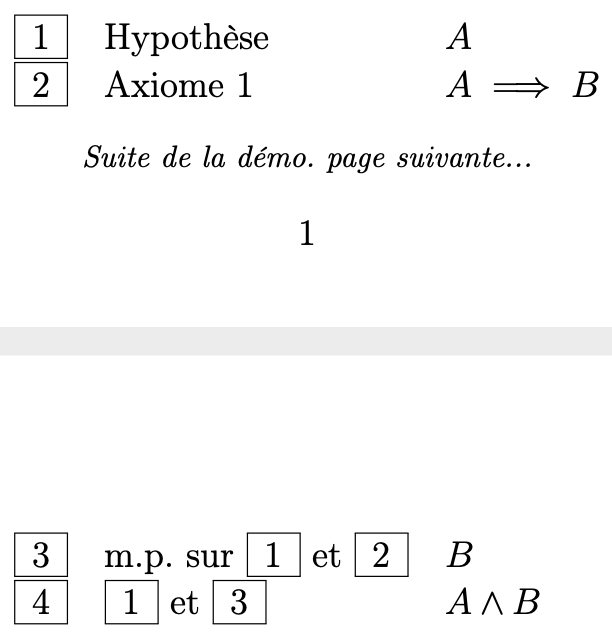
\includegraphics[scale = .5]{images/demo-explained-univ-broken[fr].png}}
\end{center}
%\section{Détailler un \og vrai \fg{} raisonnement}

\subsection{Un tableau pour le collège et le lycée} \label{tnslog-explain-hard-proof-for-youngs}


\newparaexample{Avec les réglages par défaut}

L'environnement étoilé \env{demoexplain*} est différent de l'environnement \env{demoexplain} puisqu'il sert à indiquer trois choses et non juste deux comme le montre l'exemple suivant
\footnote{
	C'est pour cela qu'est proposé une version étoilée de l'environnement et non l'utilisation d'une option de l'environnement non étoilé. 
}.
Par contre, la syntaxe est très similaire.
Notez au passage la possibilité d'utiliser \macro{newline} pour forcer un retour à la ligne dans une cellule et aussi la nécessité d'écrire les accolades de la macro sans argument \macro{demostep} lorsque la 1\iere{} case est vide \emph{(ceci est inutile lorsque l'argument optionnel est renseigné comme nous allons le vérifier dans l'exemple juste après)}.

\begin{latexex-flat}
\begin{demoexplain*}
    \demostep
        $ABC$ est un triangle \newline équilatéral 
      & Définition d'un triangle \newline équilatéral. 
      & $AB = BC = AC$
    \demostep{} % --> Ne pas oublier ici !
      & Voir l'énoncé.
      & $AB = 10 \, cm$
    \demostep
        Voir les conséquences \newline \explref*{1} et \explref*{2} .
      & Simple calcul.
      & $ABC$ a pour périmètre $30 \, cm$.
\end{demoexplain*}
\end{latexex-flat}


% ---------------------- %


\newparaexample{Avec toutes les options}

Le système de référence marche ici aussi.
Par contre \env{demoexplain*} ne propose que \verb+start+ comme clé optionnelle avec le même fonctionnement que pour \env{demoexplain}.

\begin{latexex-flat}
\begin{demoexplain*}[start = last]
    \demostep[demo-first-geo-fact]
        $ABC$ est un triangle \newline équilatéral 
      & Définition d'un triangle \newline équilatéral. 
      & $AB = BC = AC$
    \demostep[known-data]
      & Voir l'énoncé.
      & $AB = 10 \, cm$
    \demostep
        Voir les conséquences \newline
        \explref{demo-first-geo-fact} et \explref{known-data} .
      & Simple calcul.
      & $ABC$ a pour périmètre $30 \, cm$.
\end{demoexplain*}
\end{latexex-flat}


% ---------------------- %


\subsection{Un tableau sur plusieurs pages}

Un tableau devant utiliser plusieurs pages sera scindé comme ci-dessous sans perte d'information
\footnote{
	Tout le travail est fait par l'environnement \env{longtable} du package éponyme.
}.

\begin{center}
	\frame{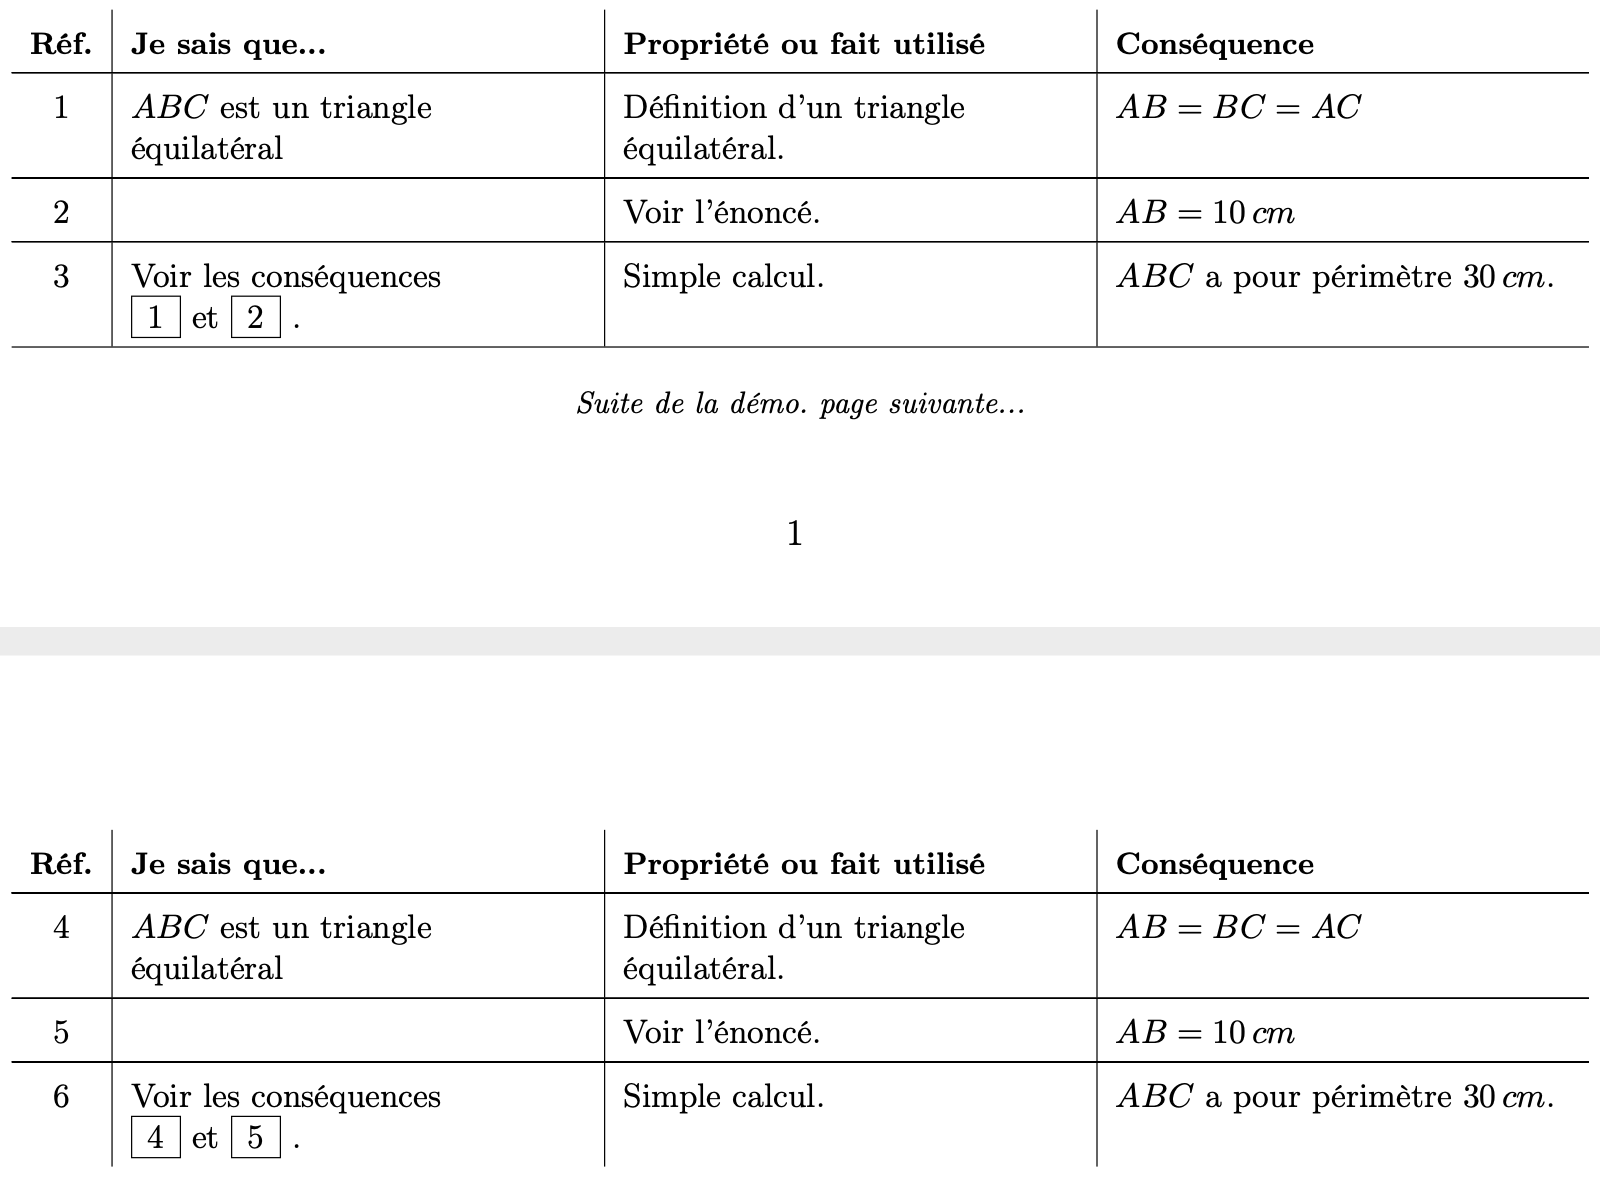
\includegraphics[scale = .5]{images/demo-explained-middleschool-broken[fr].png}}
\end{center}
%\section{Détailler un raisonnement}
\chapter{Géométrie}

\section{Points et lignes}

\subsection{Points}

\newparaexample{Sans indice}

\begin{latexex}
$\pt{I}$
\end{latexex}


% ---------------------- %


\newparaexample{Avec un indice}

\begin{latexex}
$\pt*{I}{1}$ ou
$\pt*{I}{2}$
\end{latexex}


% ---------------------- %


\subsection{Lignes}

\newparaexample{Les droites}

Dans l'exemple suivant, le préfixe \prefix{g} est pour \whyprefix{g}{éometrie} tandis que \prefix{p} est pour \whyprefix{p}{oint}.

\begin{latexex}
$\gline{A}{B}$ ,
$\gline{\pt{A}}{\pt{B}}$ ou
$\pgline{A}{B}$
\end{latexex}


% ---------------------- %


\newparaexample{Les segments}

Les macros \macro{segment} et \macro{psegment} ont un comportement similaire à \macro{gline} et \macro{pgline}.

\begin{latexex}
$\segment{A}{B}$ ,
$\segment{\pt{A}}{\pt{B}}$ ou
$\psegment{A}{B}$
\end{latexex}


% ---------------------- %


\newparaexample{Les demi-droites}

Dans l'exemple suivant, le préfixe \prefix{h} est pour \whyprefix{h}{alf}  soit \inenglish{moitié}.

\begin{latexex}
$\hgline{A}{B}$ ,
$\hgline{\pt{A}}{\pt{B}}$ ou
$\phgline{A}{B}$
\end{latexex}


% ---------------------- %


\newparaexample{D'autres demi-droites}

Ce qui suit nécessite d'utilise l'argument optionnel de \macro{gline} et \macro{pgline}. La valeur \prefix{OC} provient de \whyprefix{O}{pened} -- \whyprefix{C}{losed} soit \inenglish{ouvert -- fermé}.

\begin{latexex}
$\gline[OC]{A}{B}$ ,
$\gline[OC]{\pt{A}}{\pt{B}}$ ou
$\pgline[OC]{A}{B}$
\end{latexex}


\begin{remark}
	Les segments utilisent en fait l'option \prefix{C} et les demi-droites standard l'option \prefix{CO}.
	La valeur par défaut est \prefix{O}.
\end{remark}


% ---------------------- %


\subsection{Droites parallèles ou non}

Les opérateurs \macro{parallel} et \macro{nparallel} utilisent des obliques au lieu de barres verticales comme le montre l'exemple qui suit où \macro{stdnparallel} est un alias de \macro{nparallel} fourni par le package \verb+amssymb+, et \macro{stdparallel} est un alias de la version standard de \macro{parallel} proposée par \LaTeX{}.

\begin{latexex}
$\pgline{A}{B} \parallel \pgline{C}{D}$
au lieu de
$\pgline{A}{B}
 \stdparallel \pgline{C}{D}$

$\pgline{E}{F} \nparallel \pgline{G}{H}$
au lieu de
$\pgline{E}{F}
 \stdnparallel \pgline{G}{H}$
\end{latexex}


% ---------------------- %
\section{Vecteurs}

\subsection{Les écrire}

\newparaexample{}

\begin{latexex}
$\vect{ABCDEF}$  ,
$\vect*{e}{rot}$ ou
$\vect{e_{rot}}$
\end{latexex}


% ---------------------- %


\newparaexample{}

\begin{latexex}
$\vect{i}$ ou
$\vect*{j}{2}$
\end{latexex}


% ---------------------- %
% \section{Vecteurs}

\subsection{Norme}

Ci-dessous l'argument optionnel de \macro{vnorm} vaut \prefix{b} par défaut pour \whyprefix{b}{ig} soit \inenglish{gros} mais l'on peut aussi utiliser \prefix{s} pour \whyprefix{s}{mall} soit \inenglish*{petit}. Par contre \macro{vnorm} n'a pas d'option.

\begin{latexex}
 $\norm{\vect{i}} = \vnorm{i}$

 $\norm   {\dfrac{2}{7} \vect*{e}{k}}
= \norm[s]{\dfrac{2}{7} \vect*{e}{k}}$
\end{latexex}


\begin{remark}
	Le code \LaTeX{} pour des doubles barres extensibles ou non vient directement de ce message : \url{https://tex.stackexchange.com/a/43009/6880}.
\end{remark}


% ---------------------- %
%\section{Vecteurs}

\subsection{Produit scalaire}

Les 1\iers{} exemples utilisent une syntaxe longue mais adaptables à toutes les situations.
Voir l'exemple \ref{tnsgeo-long-dot-prod} un peu plus bas pour une écriture rapide utilisable dans certains cas.


% ---------------------- %


\newparaexample{Version classique}

\begin{latexex}
$\dotprod{\dfrac{1}{2} \vect{u}}%
         {\vect{v}}$
\end{latexex}


% ---------------------- %


\newparaexample{Version \og pédagogique mais pas écolo. \fg}

Dans l'exemple suivant l'option \prefix{b} est pour \whyprefix{b}{ullet} soit \inenglish{puce}.
Cette écriture peut être utile avec des débutants mais elle est peu pratique pour une écriture manuscrite.

\begin{latexex}
$\dotprod[b]{\dfrac{1}{2} \vect{u}}%
            {\vect{v}}$
\end{latexex}


% ---------------------- %


\newparaexample{Écriture \og universitaire \fg}

Dans l'exemple suivant l'option \prefix{p} est pour \whyprefix{p}{arenthèse} et dans \prefix{sp} le \prefix{s} est pour \whyprefix{s}{mall} soit \inenglish{petit}. On rencontre souvent cette écriture dans les cursus mathématiques universitaires.

\begin{latexex}
$\dotprod[p]{\dfrac{1}{2} \vect{u}}%
            {\vect{v}}$

$\dotprod[sp]{\dfrac{1}{2} \vect{u}}%
             {\vect{v}}$
\end{latexex}


% ---------------------- %


\newparaexample{Écriture \og à la physicienne \fg}

Dans l'exemple suivant \prefix{r} est pour \whyprefix{r}{after} soit \inenglish{chevron}. Les physiciens aiment bien cette notation.

\begin{latexex}
$\dotprod[r]{\dfrac{1}{2} \vect{u}}%
            {\vect{v}}$

$\dotprod[sr]{\dfrac{1}{2} \vect{u}}%
             {\vect{v}}$
\end{latexex}


% ---------------------- %


\newparaexample{Version courte mais restrictive} \label{tnsgeo-long-dot-prod}

Dans l'exemple suivant le préfixe \prefix{v} est pour \whyprefix{v}{ecteur}.
Notons que dans ce cas les options \prefix{sp} et \prefix{sr} n'apportent rien de nouveau.

\begin{latexex}
 $\vdotprod   {u}{v}
= \vdotprod[b]{u}{v}$
 
 $\vdotprod[r]{u}{v}
= \vdotprod[p]{u}{v}$
\end{latexex}


% ---------------------- %

%
%\newparaexample{Écriture formelle développée}
%
%Ce qui suit peut rendre service... ou pas.
%Dans l'exemple ci-dessous \prefix{exp} est pour \whyprefix{exp}{and} c'est à dire \inenglish{développer}, \prefix{c} pour \macro{cdot} et enfin \prefix{t} pour \macro{times}.
%
%\begin{latexex}
%$\dotprod[exp]{\vect{u}}{\vect{v}}$
%
%$\vdotprod[cexp]{u}{v}$
%
%$\vdotprod[texp]{u}{v}$
%\end{latexex}


% ---------------------- %
%\section{Vecteurs}

\subsection{Produit vectoriel}

\subsubsection{Écriture symbolique}

\newparaexample{Version classique en France}

\begin{latexex}
$\crossprod{\dfrac{1}{2} \vect{i}}%
           {\vect{j}}$ 
\end{latexex}


% ---------------------- %


\newparaexample{Version alternative}

La macro \macro{crossprod} possède un argument optionnel que l'on peut utiliser pour obtenir la mise en forme suivante.

\begin{latexex}
$\crossprod[t]{\dfrac{1}{2} \vect{i}}%
              {\vect{j}}$ 
\end{latexex}


% ---------------------- %


\newparaexample{Version courte mais restrictive}

\begin{latexex}
$\vcrossprod   {i}{j}$ ou
$\vcrossprod[t]{i}{j}$
\end{latexex}


% ---------------------- %


\subsubsection{Explication du mode de calcul}

Dans l'exemple suivant, le préfixe \prefix{calc} est pour \whyprefix{calc}{uler} et \prefix{v} pour \whyprefix{v}{ecteur}.

\begin{latexex}
$\calccrossprod{\vect{u}}{x }{y }{z }%
               {\vect{v}}{x'}{y'}{z'}
 =
 \vcalccrossprod{u}{x }{y }{z }%
                {v}{x'}{y'}{z'}$

$\vcalccrossprod{AB}{x_B - x_A}%
                    {y_B - y_A}%
                    {z_B - z_A}%
                {CD}{x_D - x_C}%
                    {y_D - y_C}%
                    {z_D - z_C}$
\end{latexex}


Avec un public averti on peut juste proposer les coordonnées sans les décorations comme ci-après via la version étoilée de \macro{vcalccrossprod} mais ceci fonctionne aussi avec \macro{calccrossprod}.

\begin{latexex}
$\vcalccrossprod*{u}{x }{y }{z }%
                 {v}{x'}{y'}{z'}$
\end{latexex}


Enfin si les vecteurs vous gênent il suffira d'utiliser l'option \verb+novec+ pour \verb+no+ \whyprefix{vec}{tor} soit \inenglish{pas de vecteur} comme ci-après.
Ceci fonctionne aussi pour la macro \macro{calccrossprod}.
Il peut sembler un peu lourd d'avoir des arguments pour des vecteurs non affichés mais ce choix permet à l'usage de faire des copier-coller redoutables d'efficacité !

\begin{latexex}
$\vcalccrossprod[novec]{u}{x }{y }{z }%
                       {v}{x'}{y'}{z'}
 =
 \vcalccrossprod*[novec]{u}{x }{y }{z }%
                        {v}{x'}{y'}{z'}$
\end{latexex}


% ---------------------- %


\subsubsection{Les coordonnées}

\newparaexample{Les coordonnées \og développées \fg}

Pour avoir le détail directement dans des coordonnées vous pouvez faire appel à \macro{coordcrossprod} où le préfixe \prefix{coord} fait référence à \whyprefix{coord}{onnée}
\footnote{
	En coulisse on utilise la macro \macro{coord} présentée dans la section \ref{tnsgeo-coordinates} page \pageref{tnsgeo-coordinates}. 
}.
On peut utiliser des options pour choisir certains paramètres de mise en forme.

\begin{latexex}
$\coordcrossprod{\dfrac{1}{2}x}{y }{z }%
                           {x'}{y'}{z'}$

$\coordcrossprod[vb]%
                {\dfrac{1}{2}x}{y }{z }%
                           {x'}{y'}{z'}$

$\coordcrossprod[sp,c]%
                {\dfrac{1}{2}x}{y }{z }%
                           {x'}{y'}{z'}$
\end{latexex}


\medskip

Voici les options disponibles. Nous expliquons ensuite comment les utiliser.
\begin{enumerate}
	\item \prefix{p} vient de \whyprefix{p}{arenthèses}. Ceci donnera une écriture horizontale.

	\item \prefix{b} vient de \whyprefix{b}{rackets} soit \inenglish{crochets}. Ceci donnera une écriture horizontale.

	\item \prefix{sp} et \prefix{sb} produisent des délimiteurs non extensibles en mode horizontal.
	      Ici \prefix{s} vient de \whyprefix{s}{mall} soit \inenglish{petit}.

	\item \prefix{vp} et \prefix{vb} produisent des écritures verticales.
	      Ici \prefix{v} vient de \whyprefix{v}{ertical}.

	\medskip

	\item \prefix{s} tout seul demande d'utiliser un espace pour séparer les facteurs de chaque produit.

	\item \prefix{t} tout seul demande d'utiliser \macro{times} comme opérateur de multiplication.

	\item \prefix{c} tout seul demande d'utiliser \macro{cdot} comme opérateur de multiplication.
\end{enumerate}


On peut indiquer des options vis à vis du mode vertical ou horizontal avec des délimiteurs extensibles ou non éventuellement, ou bien sur le symbole pour les produits. On peut aussi combiner deux de ces typs de choix en les séparant par une virgule ce qui fait un total de $6\times3 = 18$ combinaisons possibles.
La valeur par défaut est \verb+p,s+.


\bigskip


\textbf{Attention !}
Les produits sont rédigés stupidement. Autrement dit ce sera à vous d'ajouter des parenthèses là où il y en aura besoin sinon vous obtiendrez des horreurs comme celle ci-dessous.
    
\begin{latexex}
$\coordcrossprod[vb]%
         {x_B - x_A}{y_B - y_A}%
         {z_B - z_A}{x_D - x_C}%
         {y_D - y_C}{z_D - z_C}$
\end{latexex}

Ici nous n'avons pas d'autre choix que de corriger le tir nous-même.
Ceci étant indiqué, ce genre de situation est très rare dans la vraie vie mathématique où l'on évite d'avoir à calculer un produit vectoriel avec des expressions compliquées.
    
\begin{latexex}
$\coordcrossprod[vb]%
       {(x_B - x_A)}{(y_B - y_A)}%
       {(z_B - z_A)}{(x_D - x_C)}%
       {(y_D - y_C)}{(z_D - z_C)}$
\end{latexex}


% ---------------------- %
%\section{Vecteurs}

\subsection{Plan -- Déterminant de deux vecteurs} \label{tnsgeo-colinearity-criteria}

\newparaexample{Version décorée}

Dans l'exemple suivant, le préfixe \prefix{calc} est pour \whyprefix{calc}{uler}.

\begin{latexex}
$\calcdetplane{\vect{u}}{x }{y }%
              {\vect{v}}{x'}{y'}$
ou
$\calcdetplane{\vect{AB}}%
              {x_B - x_A}{y_B - y_A}%
              {\vect{CD}}%
              {x_D - x_C}{y_D - y_C}$
\end{latexex}


% ---------------------- %


\newparaexample{Version non décorée}

\begin{latexex}
$\calcdetplane*{\vect{u}}{x }{y }%
               {\vect{v}}{x'}{y'}$
\end{latexex}


% ---------------------- %


\newparaexample{Rédaction raccourcie pour les vecteurs}

Dans l'exemple suivant, le préfixe \prefix{v} est pour \whyprefix{v}{ecteur}.

\begin{latexex}
$\vcalcdetplane{u}{x }{y }%
               {v}{x'}{y'}
 =
 \vcalcdetplane*{u}{x }{y }%
                {v}{x'}{y'}$
\end{latexex}


% ---------------------- %


\newparaexample{Versions sans les vecteurs}

Dans l'exemple suivant, on utilise la valeur \verb+novec+ pour l'argument optionnel de \macro{vcalcdetplane} qui par défaut est \verb+vec+ pour pour \whyprefix{vec}{teur}.
À l'usage ceci permet des copier-coller très efficaces !


\begin{latexex}
 $\vcalcdetplane[novec] {u}{x }{y }%
                        {v}{x'}{y'}
= \vcalcdetplane*[novec]{u}{x }{y }%
                        {v}{x'}{y'}$
\end{latexex}


\begin{remark}
	Ce qui précède marche aussi avec les macros \macro{calcdetplane} et \macro{calcdetplane*}.
\end{remark}


% ---------------------- %


\newparaexample{Calcul développé}

Grâce à l'argument optionnel de \macro{calcdetplane} ou de \macro{vcalcdetplane} il est aussi possible d'obtenir le résultat développé du calcul comme ci-après
où \prefix{exp} est pour \whyprefix{exp}{and} soit \inenglish{développer}, \prefix{c} pour \macro{cdot} et enfin \prefix{t} pour \macro{times}.
Même si les vecteurs ne sont pas utilisés pour la mise en forme, on obtient ici une méthode très pratique à l'usage car elle permet de faire des copier-coller.

\begin{latexex}
$\vcalcdetplane[exp]{u}{x }{y }%
                    {v}{x'}{y'}$

$\vcalcdetplane[cexp]{u}{x }{y }%
                     {v}{x'}{y'}$

$\vcalcdetplane[texp]{u}{x }{y }%
                     {v}{x'}{y'}$
\end{latexex}


\begin{remark}
	Ce qui précède marche aussi avec les versions étoilées.
\end{remark}


\textbf{Attention !}
Le développement effectué est stupide. Autrement dit ce sera à vous d'ajouter des parenthèses là où il y en aura besoin sinon vous obtiendrez des horreurs comme celle qui suit.
    
\begin{latexex}
$\vcalcdetplane[exp]{AB}%
                    {x_B - x_A}%
                    {y_B - y_A}%
                    {CD}%
                    {x_D - x_C}%
                    {y_D - y_C}$
\end{latexex}

Ici nous n'avons pas d'autre choix que de régler le problème à la main. Ce genre de situation n'est pas rare dans la vraie vie mathématique.
    
\begin{latexex}
$\vcalcdetplane[exp]{AB}%
                    {(x_B - x_A)}%
                    {(y_B - y_A)}%
                    {CD}%
                    {(x_D - x_C)}%
                    {(y_D - y_C)}$
\end{latexex}


% ---------------------- %
\section{Géométrie cartésienne}

\subsection{Coordonnées} \label{tnsgeo-coordinates}

\newparaexample{Des coordonnées seules}

\verb+tnsgeo+ propose, via un argument optionnel, six façons différentes de rédiger des coordonnées seules \emph{(nous verrons après des macros pour les coordonnées d'un point et celles d'un vecteur afin de produire un code \LaTeX{} plus sémantique)}. Commençons par les écritures horizontales où vous noterez l'utilisation de \verb+|+ pour séparer les coordonnées dont le nombre peut être quelconque.

\begin{latexex}
$\coord    {\dfrac{1}{3} | -4 | 0}$ ou
$\coord[sp]{\dfrac{1}{3} | -4 | 0}$

$\coord[b] {\dfrac{1}{3} | -4 | 0}$ ou
$\coord[sb]{\dfrac{1}{3} | -4 | 0}$
\end{latexex}


Il existe en plus deux versions verticales.

\begin{latexex}
$\coord[vp]{3 | -4}$ ou
$\coord[vb]{3 | -4}$
\end{latexex}


Voici d'où viennent les noms des options.
\begin{enumerate}
	\item \prefix{p}, qui est aussi la valeur par défaut, vient de \whyprefix{p}{arenthèses}.

	\item \prefix{b} vient de \whyprefix{b}{rackets} soit \inenglish{crochets}.

	\item \prefix{s} pour \whyprefix{s}{mall} soit \inenglish{petit} permet d'avoir des délimiteurs non extensibles en mode horizontal car par défaut ils le sont.

	\item \prefix{v} pour \whyprefix{v}{ertical} demande de produire une écriture verticale.
\end{enumerate}


% ---------------------- %


\newparaexample{Coordonnées d'un point}

La macro \macro{pcoord} avec \prefix{p} pour  \whyprefix{p}{oint} prend un argument supplémentaire avant les coordonnées qui est le nom d'un point qui sera mis en forme par la macro \macro{pt}. Si vous ne souhaitez pas que \macro{pt} soit appliquée, il suffit de passer via la version étoilée \macro{pcoord*}.

\begin{latexex}
$\pcoord{A}{3 | -4 | 0 | -1}$ ou
$\pcoord*{\Sigma}{7 | 9 | 8}$
\end{latexex}


Toutes les options disponibles avec \macro{coord} le sont aussi avec  \macro{pcoord}. 

\begin{latexex}
$\pcoord[b]{A}{3 | -4 | 0 | -1}$ ou
$\pcoord*[b]{\Sigma}{7 | 9 | 8}$
\end{latexex}



% ---------------------- %


\newparaexample{Coordonnées d'un vecteur}

Le fonctionnement de \macro{vcoord} est similaire à celui de \macro{pcoord} si ce n'est que c'est la macro \macro{vect} qui sera appliquée si besoin.

\begin{latexex}
$\vcoord{u}{3 | -4}$ ou
$\vcoord*{\dfrac{1}{2} \vect{u}}%
         {3 | -4}$

$\vcoord[vp]{u}{3 | -4}$ ou
$\vcoord*[vp]{\dfrac{1}{2} \vect{u}}%
             {3 | -4}$
\end{latexex}


% ---------------------- %
% \section{Géométrie cartésienne}

\subsection{Nommer un repère}

\newparaexample{La méthode basique}

Commençons par la manière la plus basique d'écrire un repère \textit{(nous verrons d'autres méthodes qui peuvent être plus efficaces)}.

\begin{latexex}
$\axes{\pt{O} %
     | \pt{I} | \pt{J}}$
\end{latexex}


% ---------------------- %


\newparaexample{La méthode basique en version étoilée}

Dans l'exemple ci-dessous, on voit que la version étoilée produit des petites parenthèses.
\begin{latexex}
$\axes{\pt{O} %
     | \dfrac{7}{3} \vect{i} %
     | \vect{j}}$
ou
$\axes*{\pt{O} %
     | \dfrac{7}{3} \vect{i} %
     | \vect{j}}$
\end{latexex}


% ---------------------- %


\newparaexample{La méthode basique en dimension quelconque}

Il faut au minimum deux "morceaux" séparés par des barres \verb+|+, cas de la dimension $1$, mais il n'y a pas de maximum, cas d'une dimension quelconque $n > 0$.

\begin{latexex}
$\axes{\pt{O} %
     | \vect*{i}{1} %
     | \vect*{i}{2} %
     | \vect*{i}{3} %
     | \dots %
     | \vect*{i}{9} %
     | \vect*{i}{10} %
     | \vect*{i}{11} %
     | \vect*{i}{12}}$
\end{latexex}


% ---------------------- %


\newparaexample{Repère affine}

Dans l'exemple suivant, le préfixe \prefix{p} est pour \whyprefix{p}{oint}.

\begin{latexex}
$\paxes{O | I | J | K}$
au lieu de
$\axes{\pt{O} %
     | \pt{I} | \pt{J} | \pt{K}}$
\end{latexex}


% ---------------------- %


\newparaexample{Repère vectoriel (méthode 1)}

Dans l'exemple suivant, le préfixe \prefix{v} est pour \whyprefix{v}{ecteur}.

\begin{latexex}
$\vaxes{\pt{O} | i | j}$
au lieu de
$\axes{\pt{O} | \vect{i} | \vect{j}}$
\end{latexex}


% ---------------------- %


\newparaexample{Repère vectoriel (méthode 2)}

Dans l'exemple suivant, le préfixe \prefix{pv} permet de combiner ensemble les fonctionnalités proposées par les préfixes \prefix{p} et \prefix{v}.

\begin{latexex}
$\pvaxes{O | i | j}$
au lieu de
$\axes{\pt{O} | \vect{i} | \vect{j}}$
\end{latexex}


% ---------------------- %
% \section{Géométrie}

\section{Arcs circulaires}

\newparaexample{}

\begin{latexex}
$\circarc{ABCDEF}$ ,
$\circarc*{A}{rot}$ ou
$\circarc{A_{rot}}$
\end{latexex}


% ---------------------- %


\newparaexample{}

\begin{latexex}
$\circarc{i}$ ou
$\circarc*{j}{2}$
\end{latexex}


% ---------------------- %
% \section{Géométrie}

\section{Angles}

\subsection{Angles géométriques \og intérieurs \fg}

\newparaexample{}

\begin{latexex}
$\anglein {ABCDEF}$

$\anglein* {A}{rot}$

$\anglein {A_{rot}}$
\end{latexex}


% ---------------------- %


\newparaexample{Cacher les points du i et du j}

\begin{latexex}
$\anglein{i}$ et
$\anglein*{j}{2}$
\end{latexex}


% ---------------------- %
% \section{Géométrie}

%\section{Angles}

\subsection{Angles orientés de vecteurs}

\paragraph{Sans chapeau - Version longue}

L'option par défaut est \prefix{p} pour \whyprefix{p}{arenthèse}.
Dans \prefix{sp} le \prefix{s} est pour \whyprefix{s}{mall} soit \inenglish{petit}.
 
\begin{latexex}
$\angleorient    {\dfrac{1}{2} \vect{i}}%
                 {\vect{j}}$

$\angleorient[sp]{\dfrac{1}{2} \vect{i}}%
                 {\vect{j}}$
\end{latexex}


% ---------------------- %


\paragraph{Sans chapeau - Version courte mais restrictive}

Dans l'exemple suivant, le préfixe \prefix{v} est pour \whyprefix{v}{ecteur} qui permet de simplifier la saisie quand l'on a juste des vecteurs nommés avec des lettres
\emph{(notez que l'option \prefix{sp} n'apporte rien de nouveau)}.

\begin{latexex}
$\vangleorient    {i}{j}$ comme
$\vangleorient[sp]{i}{j}$
\end{latexex}


% ---------------------- %


\paragraph{Avec un chapeau}

Dans l'exemple suivant, \prefix{h} est pour \whyprefix{h}{at} soit \inenglish{chapeau}.
Notez au passage que \prefix{sh} produit juste des parenthèses petites mais ce choix de nom simplifie l'utilisation de la macro \emph{(c'est mieux que \prefix{hsp} par exemple)}.

\begin{latexex}
$\angleorient[h] {\dfrac{1}{2} \vect{i}}%
                 {\vect{j}}$

$\angleorient[sh]{\dfrac{1}{2} \vect{i}}%
                 {\vect{j}}$

$\vangleorient[h] {i}{j}$ comme
$\vangleorient[sh]{i}{j}$
\end{latexex}


% ---------------------- %
\chapter{Analyse}

\section{Constantes et paramètres}

\subsection{Constantes classiques ajoutées}

Les macros ci-dessous ne nécessitent pas d'accolades.

% List of classical constants - START

\begin{latexex}
$\ggamma$ , $\ppi$ , $\ttau$ ,
$\ee$ , $\ii$ , $\jj$ 
et $\kk$ où $\ttau = 2 \ppi$
\end{latexex}

% List of classical constants - END


\begin{remark}
	Faites attention car \verb+{\Large $\ppi \neq \pi$}+ produit {\Large $\ppi \neq \pi$}. Comme vous le constatez, les symboles ne sont pas identiques. Ceci est vraie pour toutes les constantes grecques.
\end{remark}


% ---------------------- %


\subsection{Constantes latines personnelles}

La macro \macro{param} est surtout là pour une utilisation pédagogique.

\begin{latexex}
$\param{a} x^2 + \param{b} x + \param{c}$
ou
$a x^2 + b x + c$
\end{latexex}


% ---------------------- %
\section{Une variable \og symbolique \fg{}}

Le package \verb+tnscom+ propose les macros \macro{symvar} et \macro{symvar*} qui produisent les symboles $\symvar$ et $\symvar*$ . Le nom utilisé vient de \prefix{symvar} pour \whyprefix{symb}{olic} \whyprefix{var}{iable} soit \inenglish{variable symbolique}.
Ces symboles sont utiles pour indiquer un argument symboliquement sans faire référence précisément à une ou des variables nommées.


% ---------------------- %
\section{La fonction valeur absolue}

\newparaexample*{}

\begin{latexex}
$\abs{2}$ ,
$\abs {\dfrac{3}{5}}$ ou
$\abs*{\dfrac{3}{5}}$
\end{latexex}


\begin{remark}
	Le code \LaTeX{} vient directement de ce poste : \url{https://tex.stackexchange.com/a/43009/6880}.
\end{remark}


% ---------------------- %
\section{Fonctions nommées spéciales}

\subsection{Sans paramètre}

Quelques fonctions nommées supplémentaires où le \prefix{f} dans \prefix{fch} est pour \whyprefix{f}{rench} soit \inenglish{français} \emph{(ce choix a été fait pour éviter des incompatibilités avec quelques autres packages)}. La liste complète des fonctions nommées est donnée un peu plus bas dans la section  \ref{tnsana-all-named-functions}.

\begin{latexex}
$\fch x = \cosh x$ ou
$\lg x$
\end{latexex}


% ---------------------- %


\subsection{Avec un paramètre}

Pour le moment il y a juste deux fonctions avec un paramètre. Les voici.

\begin{latexex}
$\logb{2} x = \lg x$ ou
$\expb{6} y = 6^y$
\end{latexex}


% ---------------------- %


\subsection{Toutes les fonctions nommées en plus} \label{tnsana-all-named-functions}

\vspace{-1em}

\begin{multicols}{2}
% Table of all - START
    \verb+acos+ : $\acos\dots$

    \verb+asin+ : $\asin\dots$

    \verb+atan+ : $\atan\dots$

    \verb+arccosh+ : $\arccosh\dots$

    \verb+arcsinh+ : $\arcsinh\dots$

    \verb+arctanh+ : $\arctanh\dots$

    \verb+acosh+ : $\acosh\dots$

    \verb+asinh+ : $\asinh\dots$

    \verb+atanh+ : $\atanh\dots$

    \verb+fch+ : $\fch\dots$

    \verb+fsh+ : $\fsh\dots$

    \verb+fth+ : $\fth\dots$

    \verb+afch+ : $\afch\dots$

    \verb+afsh+ : $\afsh\dots$

    \verb+afth+ : $\afth\dots$

    \verb+expb{p}+ : $\expb{p}\dots$

    \verb+logb{p}+ : $\logb{p}\dots$
% Table of all - END
\end{multicols}
\section{Définition explicite d'une fonction}

\newparaexample{Écriture par défaut}

\begin{latexex}
$\funcdef{f}{x}{x^2 + 3}%
            {I}{J}$
\end{latexex}


\begin{remark}
	Même si cela est peu utile, vous pouvez utiliser la mise en forme dans du texte pour obtenir
	$\funcdef{f}{x}{x^2 + 3}%
            {I}{J}$
    mais c'est un peu affreux.
\end{remark}

% ---------------------- %


\newparaexample{Écriture alternative}

On peut cacher le trait vertical via l'option \prefix{s} pour \whyprefix{s}{hort} soit \inenglish{court}.

\begin{latexex}
$\funcdef[s]{f}{x}{x^2 + 3}%
               {I}{J}$
\end{latexex}


% ---------------------- %


\newparaexample{Écriture en ligne}

Pour avoir tout sur une ligne, ce qui est l'idéal pour une insertion dans du texte, il suffit d'utiliser l'option \prefix{h} pour \whyprefix{h}{orizontal}.
\begin{latexex}
Soit $\funcdef[h]{f}{x}{x^2 + 3}%
                    {I}{J}$.
\end{latexex}


%% ---------------------- %
%
%
%\newparaexample{Écriture en ligne sans ensemble}
%
%Pour avoir tout sur une ligne, ce qui est l'idéal pour une insertion dans du texte, il suffit d'utiliser l'option \prefix{h} pour \whyprefix{h}{orizontal}.
%\begin{latexex}
%Soit $\funcdef[h]{f}{x}{x^2 + 3}%
%                    {I}{J}$.
%\end{latexex}


% ---------------------- %
\section{Limite}

\newparaexample{Cas minimaliste}

Notez ci-dessous que le rendu de la limite via \macro{limit} se fait toujours en mode \macro{displaystyle} pour l'opérateur de limite.

\begin{latexex}
$\limit{f(x)}{x}{0} = \frac{1}{2}$
\end{latexex}


\begin{remark}
	\verb#\lim\limits_{x \rightarrow 0} f(x)# produit 
	$\lim\limits_{x \rightarrow 0} f(x)$ contre 
	$\limit{f(x)}{x}{0}$ ci-dessus.
\end{remark}



% ---------------------- %


\newparaexample{Avec des conditions}

Ce 2\ieme{} exemple devrait rendre intéressante la macro \macro{limit} qui permet d'ajouter facilement plusieurs conditions comme le montre la 2\ieme{} limite
\footnote{
	En pratique, on utilise généralement au maximum une condition.
}.

\begin{latexex}
$\limit{f(x)}{x}{0 | x > 0}$ ou
$\limit{f(z)}{z}%
       {0 | z \in \Omega | \abs{z} < 3}$
\end{latexex}


% ---------------------- %


\newparaexample{Ajout de parenthèses}

Les options \verb#p# et \verb#sp# permettent d'ajouter facilement des parenthèses extensibles ou non autour de la fonction. 
Indiquons que \prefix{sp} est pour \whyprefix{s}{mall} \whyprefix{p}{arenthesis} soit \inenglish{petites parenthèses}.

\begin{latexex}
$\displaystyle\limit[p] {\frac{1}{x}}{x}
                        {0 | x > 0}$
ou
$\displaystyle\limit[sp]{\frac{1}{x}}{x}
                        {0 | x > 0}$
\end{latexex}


% ---------------------- %
\section{Calcul différentiel}

\subsection{\texorpdfstring{Les opérateurs $\pp{}$ et $\dd{}$}%                           {Les opérateurs "d rond" et "d droit"}}
                           {Les opérateurs "d rond" et "d droit"}}

Voici deux opérateurs utiles aussi bien pour du calcul différentiel que du calcul intégral. 

\begin{latexex}
$\dd{t} = \dd[1]{t}$ ou $\dd[n]{x}$

$\pp{t} = \pp[1]{t}$ ou $\pp[n]{x}$
\end{latexex}


% ---------------------- %


\subsection{Dérivations totales d'une fonction -- Version longue avec une variable}

\newparaexample{Différentes écritures possibles}

La macro \macro{der} est stricte du point de vue sémantique car on doit lui fournir la fonction, l'ordre de dérivation et la variable de dérivation
\emph{(voir la section \ref{tnsana-short-der} qui présente la macro \macro{sder} permettant une rédaction efficace pour obtenir $\sder[e]{f}{1}$ ou $\sder{f}{1}$)}.
Voici plusieurs mises en forme faciles à taper via l'option de \macro{der}.
Attention bien entendu à n'utiliser l'option par défaut \prefix{u} ou l'option \prefix{d} qu'avec un ordre de dérivation de valeur naturelle connue !

\begin{latexex}
 $\der   {f}{x}{3}
= \der[e]{f}{x}{3}
= \der[d]{f}{x}{3}$

 $\der[i] {u}{x}{k}
= \der[f] {u}{x}{k}
= \der[sf]{u}{x}{k}$
\end{latexex}


On peut aussi ajouter autour de la fonction des parenthèses extensibles ou non sauf même si cela n'est pas utile pour le mode \prefix{d} \emph{(voir juste après le mode \prefix{bd})}.
Ci-dessous on montre au passage une écriture du type \emph{\og opérateur fonctionnel \fg} : voir la section \ref{tnsana-ope-total-der} page \pageref{tnsana-ope-total-der} à ce sujet.

\begin{latexex}
 $\der[osf,sp]{\frac{1}{2}  uv}{x}{k}
= \der[of,p]  {\dfrac{1}{2} uv}{x}{k}$
\end{latexex}


Avec l'option \prefix{d} les parenthèses seules sont sans utilité car on peut obtenir des choses non souhaitées comme $\der[d, p]{u + v}{x}{2}$.
À la place on utilisera l'option \prefix{bd} où le \prefix{b} est pour \whyprefix{b}{racket} soit \inenglish{crochet}. Notez au passage que \prefix{p} et \prefix{sp} restent utilisables.

\begin{latexex}
 $\der[bd]   {\frac{1}{2}  uv}{x}{2}
= \der[bd,p] {\frac{1}{2}  uv}{x}{2}
= \der[bd,sp]{\dfrac{1}{2} uv}{x}{2}$
\end{latexex}


\begin{remark}
	Expliquons les valeurs des options.
	\begin{enumerate}
		\item \prefix{u}, la valeur par défaut, est pour \whyprefix{u}{suel} soit l'écriture avec les primes. Cette option ne marchera pas avec un nombre symbolique de dérivations. 

		\item \prefix{e} est pour \whyprefix{e}{xposant}.

		\item \prefix{i} est pour \whyprefix{i}{ndice}.

		\item \prefix{d} est pour \whyprefix{d}{ot} soit \inenglish{point}.

		\item \prefix{bd} est pour \whyprefix{b}{racket} \whyprefix{d}{ot} où \inenglish*{bracket} est pour \inenglish{crochet}.

		\medskip
		
		\item \prefix{f} est pour \whyprefix{f}{raction} avec aussi \prefix{sf} pour une écriture réduite où \prefix{s} est pour \whyprefix{s}{mall} soit \inenglish{petit}.

		\item \prefix{of} et \prefix{osf} utilisent le préfixe \prefix{o} pour \whyprefix{o}{pérateur}.
		
		\medskip
		
		\item \prefix{p} est pour \whyprefix{p}{arenthèse} : dans ce cas les parenthèses seront extensibles. Le fonctionnement est différent avec l'option \prefix{d} comme nous l'avons vu avant.

		\item \prefix{sp} est pour des parenthèses non extensibles. Là aussi le fonctionnement est différent avec l'option \prefix{d}.
	\end{enumerate}
\end{remark}


% ---------------------- %


\newparaexample{Pas de uns inutiles}

\begin{latexex}
 $\der[i ]{u}{x}{1}
= \der[f ]{u}{x}{1}
= \der[sf]{u}{x}{1}
= \der[of]{u}{x}{1}$
\end{latexex}


\begin{remark}
	Voici comment forcer les exposants $1$ si besoin. Fonctionnel mais très moche...

	\begin{latexex}
 $\der[i ]{u}{x}{\,\!1}
= \der[f ]{u}{x}{\,\!1}
= \der[sf]{u}{x}{\,\!1}
= \der[of]{u}{x}{\,\!1}$
\end{latexex}
\end{remark}

% ---------------------- %


\subsection{Dérivations totales d'une fonction -- Version courte sans variable} \label{tnsana-short-der}

Dans l'exemple suivant le code manque de sémantique car on n'indique pas la variable de dérivation.
Ceci étant dit à l'usage la macro \macro{sder} rend de grands services.
Ici le préfixe \prefix{s} est pour \whyprefix{s}{imple} voire \whyprefix{s}{impliste}...
Voici des exemples où de nouveau l'option par défaut \prefix{u} et l'option \prefix{d} ne seront fonctionnelles qu'avec un ordre de dérivation de valeur naturelle connue !


\newparaexample{}

\begin{latexex}
 $\sder{f}{1} = \der{f}{x}{1}$

 $\sder   {f}{3}
= \sder[e]{f}{3}
= \sder[d]{f}{3}$
\end{latexex}


\newparaexample{}

\begin{latexex}
 $\sder[sp] {\dfrac{1}{2} uv}{2}
= \sder[e,p]{\dfrac{1}{2} uv}{2}
= \sder[bd] {\dfrac{1}{2} uv}{2}$
\end{latexex}


\begin{remark}
	Ici les seules options disponibles sont \prefix{u}, \prefix{e}, \prefix{b}, \prefix{bd}, \prefix{p} et \prefix{sp}.
\end{remark}


% ---------------------- %


\subsection{L'opérateur de dérivation totale} \label{tnsana-ope-total-der}

Ce qui suit peut rendre service au niveau universitaire.
Les options possibles sont \verb+f+, valeur par défaut, \verb+sf+ et \verb+i+ avec les mêmes significations que pour la macro \macro{der}.

\begin{latexex}
 $\derope    {x}{k}
= \derope[sf]{x}{k}
= \derope[i] {x}{k}$
\end{latexex}


Ici non plus il n'y a pas de uns inutiles mais l'astuce \verb+\,\!1+ reste utilisable.

\begin{latexex}
 $\derope    {x}{1}
= \derope[sf]{x}{1}
= \derope[i] {x}{1}$
\end{latexex}


% ---------------------- %
%\section{Calcul différentiel}

\subsection{Dérivations partielles}

\newparaexample{Différentes écritures}

La macro \macro{pder}
\footnote{
	\macro{partial} existe déjà pour obtenir $\partial$.
}
avec \prefix{p} pour \whyprefix{p}{artielle}
permet de rédiger des dérivées partielles en utilisant facilement plusieurs mises en forme via une option qui vaut \verb+f+ par défaut.
Cette macro attend une fonction, les dérivées partielles effectuées et l'ordre total de dérivation.
Voici deux types de mise en forme classiques où vous noterez comment \verb+x | y^2+ est interprété.

\begin{latexex}
 $\pder    {f}{x | y^2}{3}
= \pder[sf]{f}{x | y^2}{3}$
\end{latexex}


Il existe en plus deux notations indicielles données en exemple ci-dessous.
Notez qu'avec l'option \verb+ei+ l'exposant total n'est pas imprimé et que les exposants partiels doivent être des naturels connus.

\begin{latexex}
 $\pder[i] {f}{x | y^2}{3}
= \pder[ei]{f}{x | y^2}{3}$
\end{latexex}


\begin{remark}
	L'option \verb+ei+ ne marche pas avec des variables indicées pour le moment.
\end{remark}


\medskip


On peut aussi ajouter autour de la fonction à différencier des parenthèses extensibles ou non via \verb+p+ et \verb+sp+ respectivement.
Ci-dessous on montre aussi une écriture du type \emph{\og opérateur fonctionnel \fg} : voir la section \ref{tnsana-ope-partial-der} page \pageref{tnsana-ope-partial-der} à ce sujet.

\begin{latexex}
 $\pder[of,sp] {u + v}{x | y^2}{}
= \pder[osf,sp]{u + v}{x | y^2}{}
= \pder[i,sp]  {u + v}{x | y^2}{}$
\end{latexex}


\begin{remark}
	Les options disponibles sont 
	\verb+f+, \verb+sf+, \verb+of+, \verb+osf+, \verb+p+ et \verb+sp+  
	avec des significations similaires à celles pour la macro \macro{der}
	auxquelles s'ajoutent \verb+i+ et \verb+ei+ pour les écritures indicielles où le \prefix{e} dans \prefix{ei} est pour \whyprefix{e}{xpand} soit \inenglish{développer}.
\end{remark}


% ---------------------- %


\newparaexample{Pas de uns inutiles}

\begin{latexex}
 $\pder    {u}{x}{1}
= \pder[sf]{u}{x}{1}
= \pder[i] {u}{x}{1}$
\end{latexex}


\begin{remark}
	Rappelons que pour obtenir $\pder[i]{u}{x}{\,\!1}$ on peut taper \verb+\pder[i]{u}{x}{\,\!1}+.
\end{remark}


% ---------------------- %


\subsection{L'opérateur de dérivation partielle} \label{tnsana-ope-partial-der}

Ce qui suit peut rendre service au niveau universitaire.
Les options possibles sont \verb+f+, valeur par défaut, \verb+sf+ et \verb+i+ avec les mêmes significations que pour la macro \macro{pder}.

\begin{latexex}
 $\pderope    {x | y^2}{3}
= \pderope[sf]{x | y^2}{3}
= \pderope[i] {x | y^2}{3}$
\end{latexex}


% ---------------------- %
% \section{Analysis}

\section{Tableaux de variation et de signe}

\subsection{Les bases de \texttt{tkz-tab}}

\paragraph{Comment ça marche ?}

Pour les tableaux de variation et de signe non décorés, tout le boulot est fait par le package \verb+tkz-tab+.
Ce package est utilisé avec les réglages par défaut \emph{\og maison \fg} suivants via l'utilisation de \macro{tkzTabSetup}.

\begin{enumerate}
	\item \verb+arrowstyle = triangle 60+ permet d'obtenir des pointes de flèche plus visibles.
	
	\item \verb+doubledistance = 3pt+ améliore la visibilité des doubles barres pour les valeurs interdites.
\end{enumerate}


 

\medskip

Nous donnons quelques exemples classiques d'utilisation proches ou identiques de certains proposés dans la documentation de \verb+tkz-tab+ \emph{(les codes ont été mis en forme pour faciliter la compréhension de la syntaxe à suivre)}.
Reportez vous à la documentation de \verb+tkz-tab+ pour des compléments d'information : vous y trouverez des réglages très fins.


% ---------------------- %


\newparaexample{Avec des signes}

\inputlatexexcodeafter{tikz/cos-sign.tkz}


% ---------------------- %


\newparaexample{Avec des variations (sans cadre)}

\inputlatexexcodeafter{tikz/basic-var.tkz}


% ---------------------- %


\newparaexample{Variations via une dérivée (sans cadre)}

\inputlatexexcodeafter{tikz/sin-var-via-cos.tkz}


% ---------------------- %


\newparaexample{Une image intermédiaire avec une seule flèche}

\inputlatexexcodeafter{tikz/inter-img.tkz}


% ---------------------- %


\newparaexample{Valeurs interdites et valeurs supplémentaires}

\inputlatexexcodeafter{tikz/illegal-n-inter-img-1.tkz}


Voici un autre exemple pour comprendre comment utiliser \macro{tkzTabVal} avec en plus l'option \verb+draw+ qui peut rendre service.

\inputlatexexcodeafter{tikz/illegal-n-inter-img-2.tkz}


% ---------------------- %


\newparaexample{Signe à partir des variations (un peu de pédagogie...)}

Il est assez facile de produire des choses très utiles pédagogiquement comme ce qui suit en se salissant un peu les mains avec du code TikZ.

\begin{center}
	\input{tikz/align-sign-from-var-1.tkz}
\end{center}

On déduit du tableau précédent le signe de la fonction $f$.

\begin{center}
	\input{tikz/align-sign-from-var-2.tkz}
\end{center}


Voici le code du 1\ier{} tableau où le placement de la valeur $3$ au milieu entre $2$ et $+\infty$ va nous simplifier le travail pour le 2\ieme{} tableau.

\medskip

\inputlatexexalone{tikz/align-sign-from-var-1.tkz}


Pour produire le code du 2\ieme{} tableau il a fallu utiliser au préalable ce qui suit en activant l'option \verb@help@ qui demande à \verb@tkz-tab@ d'afficher les noms de noeuds au sens TikZ qui ont été créés.
Ceci permet alors d'utiliser ces noeuds pour des dessins TikZ faits maison
\footnote{
    C'est grâce à ce mécanisme que \prefix{tnsana} peut proposer des outils explicatifs des tableaux de signe : voir la section suivante.
}.
	

\inputlatexexcodeafter{tikz/node-name.tkz}


Maintenant que les noms des noeuds sont connus, il devient facile de produire le code ci-après.
Bien noter l'usage de valeurs utiles \og vides \fg{} de $x$ ainsi que les mystiques \verb@\node at ($(A)!0.5!(B)$)@ permettant de placer un noeud au milieu entre les deux noeuds \verb@A@ et \verb@B@. 

\inputlatexexalone{tikz/align-sign-from-var-2.tkz}


% ---------------------- %


\newparaexample{Convexité et concavité symbolisées dans les variations}

Voici un autre exemple s'utilisant la machinerie TikZ afin d'indiquer dans les variations la convexité et la concavité via des flèches incurvées \emph{(cette convention est proposée dans la sous-section \emph{\og Exemple utilisant l'option \macro{help} \fg} de la section \emph{\og Gallerie \fg}  de la documentation de \prefix{tkz-tab})}.

\begin{center}
\begin{tikzpicture}
    \tkzTabInit[
        espcl = 3,
%        help       % <-- Pour voir les noms des noeuds.
    ]{
        $x$   / 0.75 ,
        $f''$ / 1    ,
        $f'$  / 2    ,
        $f$   / 3
    }{
                $-\infty$          , $0$          , $+\infty$
    }
    \tkzTabLine{               , - , z        , + ,              }
    \tkzTabVar {+ / $+\infty$      , - / $-2$     , + / $+\infty$}

    \tkzTabVal[draw]{1}{2}{.5}{$x_1$}{$0$}
    \tkzTabVal[draw]{2}{3}{.5}{$x_2$}{$0$}

    \begin{scope}[->, > = triangle 60]
        \coordinate (Middle1) at ($(N13)!0.5!(N14)$);
        \coordinate (Middle2) at ($(N23)!0.5!(N24)$);
        \coordinate (Middle3) at ($(N33)!0.5!(N34)$);
        \path (N13) -- (N23) node[midway,below=6pt](N){};
        %
        \draw ([above=6pt]Middle1)
              to [bend left=45] ([left=1pt]N);
        \draw ([right=3pt]N)
              to [bend left=45] ([above=6pt]Middle2) ;
        \draw ([below right=3pt]Middle2)
              to [bend left=-45] ([above=6pt]M24) ;
        \draw ([above right=6pt]M24)
              to [bend right=40] ([below left=6pt]Middle3);
    \end{scope}
\end{tikzpicture}
\end{center}

Le code utilisé est le suivant.

\begin{latexex-alone}
\begin{tikzpicture}
    \tkzTabInit[
        espcl = 3,
%        help       % <-- Pour voir les noms des noeuds.
    ]{
        $x$   / 0.75 ,
        $f''$ / 1    ,
        $f'$  / 2    ,
        $f$   / 3
    }{
                $-\infty$          , $0$          , $+\infty$
    }
    \tkzTabLine{               , - , z        , + ,              }
    \tkzTabVar {+ / $+\infty$      , - / $-2$     , + / $+\infty$}

    \tkzTabVal[draw]{1}{2}{.5}{$x_1$}{$0$}
    \tkzTabVal[draw]{2}{3}{.5}{$x_2$}{$0$}

    \begin{scope}[->, > = triangle 60]
        \coordinate (Middle1) at ($(N13)!0.5!(N14)$);
        \coordinate (Middle2) at ($(N23)!0.5!(N24)$);
        \coordinate (Middle3) at ($(N33)!0.5!(N34)$);
        \path (N13) -- (N23) node[midway,below=6pt](N){};
        %
        \draw ([above=6pt]Middle1)
              to [bend left=45] ([left=1pt]N);
        \draw ([right=3pt]N)
              to [bend left=45] ([above=6pt]Middle2) ;
        \draw ([below right=3pt]Middle2)
              to [bend left=-45] ([above=6pt]M24) ;
        \draw ([above right=6pt]M24)
              to [bend right=40] ([below left=6pt]Middle3);
    \end{scope}
\end{tikzpicture}
\end{latexex-alone}
%% \section{Analysis}
%
%\section{Tableaux de variation et de signe}

\subsection{Décorer facilement un tableau}

\subsubsection{Motivation}

Considérons le tableau suivant et imaginons que nous voulions l'expliquer à un débutant.

\begin{center}
	\input{tikz/deco-basic-1.tkz}
\end{center}

Deux options s'offrent à nous pour justifier comment a été rempli le tableau.

\begin{enumerate}
    \item Classiquement on résout par exemple juste les deux inéquations $2 x - 3 > 0$ et $-x + 5 > 0$ puis on complète les deux premières lignes
    \footnote{
        Notons que cette approche est un peu scandaleuse car il faudrait en toute rigueur aussi résoudre
        $2 x - 3 < 0$ , $-x + 5 < 0$ , $2 x - 3 = 0$ et $-x + 5 = 0$.
        Personne ne le fait car l'on pense aux variations d'une fonction affine. Dans ce cas pourquoi ne pas juste utiliser ce dernier argument?
        C'est ce que propose la 2\ieme{} méthode.
    }
    pour en déduire la dernière via la règle des signes d'un produit.

    \item On peut proposer une méthode moins sujette à la critique qui s'appuie sur la représentation graphique d'une fonction affine en produisant le tableau suivant.
\end{enumerate}

\begin{center}
	\input{tikz/deco-basic-2.tkz}
\end{center}


Pour produire le 2\ieme{} tableau, en plus du code \verb#tkz-tab# pour le tableau de signe
\footnote{
	Nous avons utilisé les réglages optionnels
	\texttt{lgt = 3.5} et \texttt{espcl = 2.5} de \macro{tkzTabInit}
	pour avoir de la place dans la 1\iere{} colonne pour le dernier produit
	et aussi réduire la largeur des colonnes pour les signes.
},
il a fallu ajouter les lignes données ci-dessous où sont utilisées les macros     \macro{backLine}, \macro{graphSign} et \macro{comLine} proposées par \verb+tnsana+ \emph{(la syntaxe simple à suivre sera expliquée dans les trois sections suivantes)}.
	Indiquons que les lignes pour les signes doivent utiliser un coefficient minimal de \texttt{1.5} pour la hauteur afin d'éviter la superposition des graphiques.

\medskip

\inputlatexexalone{tikz/deco-basic-2-short.tkz}


\begin{remark}
	Il est aussi possible de décorer une ligne de variation comme cela sera montré dans l'exemple \ref{tnsana-graphsign-com-two-lines} page \pageref{tnsana-graphsign-com-two-lines}. 
\end{remark}


% ---------------------- %


\subsubsection{Ajouter une couleur de fond à une ligne}

La modification de la couleur de fond d'une ligne se fait via la macro \macro{backLine}
\footnote{
    L'auteur de \prefix{tnsana} n'est absolument pas un fan de la casse en bosses de chameau mais par souci de cohérence avec ce que propose \prefix{tkz-tab} le nom \macro{backLine} a été proposé à la place de \macro{backline}.
}
pour \whyprefix{back}{ground} \prefix{of the line} soit \inenglish{fond de la ligne}.
Cette macro possède un argument optionnel et un obligatoire.

\begin{itemize}[label=\small\textbullet, itemsep=.25em]
    \item \textit{L'argument optionnel : choix de la couleur de fond.}
          
          \smallskip
          
          Ci-dessus nous avons utilisé la couleur par défaut qui est  \verb#gray!30#.


    \medskip
    \item \textit{L'argument obligatoire : les numéros de ligne séparés par des virgules.}
          
          \smallskip
          
          La numérotation des lignes commence à $0$ comme en informatique. Ainsi \verb#\backLine{0,3}# ajoute une couleur de fond à la ligne des valeurs utiles de $x$ et à la 3\ieme{} ligne de signes, ou moins intuitivement à la (3+1)\ieme{} ligne du tableau.
\end{itemize}



% ---------------------- %


\subsubsection{Commenter une ligne} \label{tnsana-comment-tab-sign}

L'ajout de commentaires courts se fait via la macro \macro{comLine} pour \whyprefix{com}{ment a} \prefix{line} soit \inenglish{commenter une ligne}.
Cette macro possède un argument optionnel et deux obligatoires.

\begin{itemize}[label=\small\textbullet, itemsep=.25em]
    \item \textit{L'argument optionnel : choix de la couleur du texte.}
          
          \smallskip
          
          Ci-dessus nous avons utilisé \verb#\comLine[gray]{0}{...}# pour avoir un texte en gris.


    \item \textit{Le 1\ier{} argument : le numéro de ligne \emph{(comme pour \macro{backLine})}.}


    \item \textit{Le 2\ieme{} argument : texte du commentaire.}
          
          \smallskip
          
          Par défaut aucun retour à la ligne n'est possible.
          Si besoin se reporter à l'exemple \ref{tnsana-graphsign-com-two-lines},  page \pageref{tnsana-graphsign-com-two-lines} section \ref{tnsana-graphsign-examples}, où est montré comment écrire sur plusieurs lignes.
\end{itemize}


% ---------------------- %


\subsubsection{Graphiques pour expliquer des signes}

Pour le moment, la macro \macro{graphSign} propose différents types de graphiques de fonctions dites de référence.
Avant de voir ce qui est proposé rappelons que la convention est de prendre $0$ pour numéro de la toute 1\iere{} ligne contenant les valeurs utiles de la variable.

\begin{enumerate}
    \item \textbf{\itshape Fonctions affines non constantes avec une contrainte.}
          
          \smallskip

          Pour les fonctions du type $f(x) = a x + b$ avec $a \neq 0$, nous devons connaître le signe de $a$ et la racine $r$ de $f$.
          Le codage est simple : considérons par exemple \verb#\graphSign{2}{ax+b, an}{$5$}#.
		  %
          \begin{itemize}[label=\small\textbullet, itemsep=.25em]
          		\item \textit{1\ier{} argument $2$.}

		              \smallskip
		              Ceci indique d'ajouter le graphique dans la 2\ieme{} ligne de signes.


          		\item \textit{\texttt{ax+b} dans le 2\ieme{} argument.}

		              \smallskip
		              Ce code sans espace indique une fonction affine.
		              

          		\item \textit{\texttt{an} dans le 2\ieme{} argument.}

		              \smallskip
		              Ce code venant de \prefix{a négatif} ajoute la condition $a < 0$.

		
				\item \textit{3\ieme{} argument $5$.}

		              \smallskip
		              Ceci donne la racine.
          \end{itemize}

          Donc pour ajouter dans la 4\ieme{} ligne de signe le graphique de $f(x) = 3x$, on utilisera dans ce cas \verb#\graphSign{4}{ax+b, ap}{$0$}# où \prefix{ap} pour \prefix{a positif} code la condition $a > 0$.


    % ==================== %


    \bigskip
    \item \textbf{\itshape Fonctions trinômiales du 2\ieme{} degré avec deux contraintes.}
          
          \smallskip

          Pour les fonctions du type $f(x) = a x^2 + b x + c$ avec $a \neq 0$, en plus du signe de $a$ nous devons connaître celui du discriminant $\Delta = b^2 - 4ac$, ce dernier pouvant être nul, sans oublier les racines réelles éventuelles.
		  Voyons comment coder ce genre de chose via par exemple \verb#\graphSign{5}{ax2+bx+c, an, dp}{$r_1$}{$r_2$}#.
		  %
          \begin{itemize}[label=\small\textbullet, itemsep=.25em]
          		\item \textit{1\ier{} argument $5$.}

		              \smallskip
		              On indique la 5\ieme{} ligne de signes.

          		\item \textit{\texttt{ax2+bx+c} dans le 2\ieme{} argument.}

		              \smallskip
		              Ce code sans espace indique un trinôme du 2\ieme{} degré.


          		\item \textit{\texttt{an} dans le 2\ieme{} argument \emph{(comme avant).}}


          		\item \textit{\texttt{dp} dans le 2\ieme{} argument.}

		              \smallskip
		              Ce code venant de \prefix{discriminant positif} ajoute la condition $\Delta > 0$.
		              En plus de \prefix{dn} et \prefix{dp} il y a aussi \prefix{dz} pour \prefix{discriminant zéro}.
		
		
				\item \textit{3\ieme{} et 4\ieme{} arguments $r_1$ et $r_2$.}

		              \smallskip
		              Ceci donne les deux racines réelles avec obligatoirement $r_1 < r_2$.
          \end{itemize}


          Ainsi pour indiquer dans la 3\ieme{} ligne de signe la courbe relative à $f(x) = - 4 x^2$, on utilisera \verb#\graphSign{3}{ax2+bx+c, an, dz}{$0$}#.


          \smallskip

          Enfin le graphique associé au trinôme $f(x) = 7 x^2 + 3$, qui est sans racine réelle, s'obtiendra dans la 4\ieme{} ligne de signe via \verb#\graphSign{4}{ax2+bx+c, ap, dn}#.


    % ==================== %


    \bigskip
    \item \textbf{\itshape Fonctions sans contrainte.}
          
          \smallskip

          Voici ce qui est disponible via \verb#\graphSign{noligne}{codefonc}# où les valeurs possibles de \verb#codefonc# sont les suivantes.
          
		  \begin{center}
		  	  \begin{tabular}{r|c|c|c|c|c|c}
				  \verb+codefonc+
				      &  \verb#x2#
				      &  \verb#sqrt#
				      &  \verb#1/x#
				      &  \verb#abs#
				      &  \verb#exp#
				      &  \verb#ln#
				  \\
				  \hline
				  $f(x)$
				      &  $x^{2\vphantom{X^{X^X}}}$
				      &  $\sqrt x$
				      &  $\frac1x$
				      &  $\abs x$
				      &  $\exp x$
				      &  $\ln x$ 
		  	  \end{tabular}
		  \end{center}
\end{enumerate}
%% \section{Analysis}
%
%\section{Tableaux de variation et de signe}

\subsubsection{Quelques exemples}  \label{tnsana-graphsign-examples}

\newparaexample{Avec une parabole}

Il devient très facile de proposer un tableau décoré comme le suivant.

\begin{center}
	\input{tikz/deco-parabola.tkz}
\end{center}


En plus des deux exemples de schémas de paraboles, il faut noter dans le code supplémentaire ajouté l'utilisation de \verb#\kern1.75em# dans \verb#\comLine[gray]{0}{\kern1.75em Schémas}# afin de mettre un espace horizontal précis pour centrer à la main le texte \emph{\og Schémas \fg} \emph{(un peu sâle mais ça marche)}.

\medskip

\inputlatexexalone{tikz/deco-parabola-short.tkz}


% ---------------------- %


\newparaexample{Avec des fonctions sans paramètre}

Voici un 1\ier{} tableau avec certaines des fonctions sans paramètre.

\begin{center}
	\input{tikz/deco-ref-1.tkz}
\end{center}

Le code correspondant est le suivant.

\medskip

\inputlatexexalone{tikz/deco-ref-1-short.tkz}

\medskip

Voici un 2\ieme{} tableau avec les fonctions sans paramètre manquantes ci-dessus.

\begin{center}
	\input{tikz/deco-ref-2.tkz}
\end{center}

Le code correspondant est le suivant.

\medskip

\inputlatexexalone{tikz/deco-ref-2-short.tkz}


% ---------------------- %


\newparaexample{Commenter des variations} \label{tnsana-graphsign-com-two-lines}

Pour finir, indiquons que les outils de décoration marchent aussi pour les tableaux de variation.
Voici un exemple possible d'utilisation où les retours à la ligne ont été obtenus affreusement, ou pas, via \verb#\parbox{11.5em}{...}#.

\begin{center}
	\input{tikz/deco-var.tkz}
\end{center}
%% \section{Analysis}
%
%\section{Tableaux de variation et de signe}
\section{Calcul intégral}

\subsection{Le symbole standard revisité}

Commençons par un point important : le package réduit les espacements entres des symboles $\int$ successifs. Voici un exemple.

\begin{latexex}
$\displaystyle
 \int \int \int 
 F(x;y;z) \dd{x} \dd{y} \dd{z}$

$\displaystyle
 \int_{a}^{b} \int_{c}^{d} \int_{e}^{f} 
 F(x;y;z) \dd{x} \dd{y} \dd{z}$
\end{latexex}


\begin{remark}
	Par défaut, \LaTeX{} affiche
	$\displaystyle
	 \stdint \stdint \stdint
	 F(x;y;z) \dd{x} \dd{y} \dd{z}$
    et
    $\displaystyle
	 \stdint_{a}^{b} \stdint_{c}^{d} \stdint_{e}^{f}
     F(x;y;z) \dd{x} \dd{y} \dd{z}$.
    Nous avons obtenu ce résultat en utilisant \macro{stdint} qui est l'opérateur proposé de façon standard par \LaTeX.
\end{remark}


% ---------------------- %


\subsection{Un opérateur d'intégration clés en main}

\newparaexample{À quoi bon ?}

Le 1\ier{} exemple qui suit semblera être une hérésie pour les habitués de \LaTeX{} mais rappelons que le but de \verb+tnsana+ est de rendre les documents facilement modifiables globalement ou localement comme le montre le 2\ieme{} exemple.

\begin{latexex}
 $\displaystyle
  \integrate{f(x)}{x}{a}{b}
= \int_{x=a}^{x=b} f(x) \dd{x}$

 $\displaystyle
  \integrate*{f(x)}{x}{a}{b}
= \integrate{f(x)}{x}{a}{b}$
\end{latexex}


\newparaexample{Le mode \texttt{displaystyle}}

La macro \macro{dintegrate*} présentée ci-dessous possède aussi une version non étoilée \macro{dintegrate}.

\begin{latexex}
 $\dintegrate*{f(x)}{x}{a}{b}
= \integrate*{f(x)}{x}{a}{b}$
\end{latexex}


% ---------------------- %


\subsection{L'opérateur \og crochet \fg}

\newparaexample{}

\begin{latexex}
 $\hook{F(x)}{x}{a}{b}
= F(b) - F(a)$

 $\dintegrate*{f(x)}{x}{a}{b}
= \hook*{F(x)}{x}{a}{b}$

\end{latexex}


\begin{remark}
	Il faut savoir que \macro{hook} signifie \inenglish{crochet} mais la bonne traduction du terme mathématique est en fait \emph{\og square bracket \fg}. Ceci étant dit l'auteur de \verb+tnsana+ trouve plus efficace d'utiliser \macro{hook} comme nom de macro.
\end{remark}


% ---------------------- %


\newparaexample{Des crochets non extensibles}

Dans l'exemple suivant, on utilise l'option \prefix{sb} pour \whyprefix{s}{mall} \whyprefix{b}{rackets} soit \inenglish{petits crochets}. Les options sont disponibles à la fois pour \macro{hook} et \macro{hook*}.


\begin{latexex}
 $\hook*{\dfrac{x - 1}{5 + x^2}}{x}%
        {a}{b}
= \hook*[sb]%
        {\dfrac{x - 1}{5 + x^2}}{x}%
        {a}{b}$
\end{latexex}


% ---------------------- %


\newparaexample{Un trait vertical épuré}

Via les options \prefix{r} et \prefix{sr} pour \whyprefix{s}{mall} et \whyprefix{r}{ull} soit \inenglish*{petit} et \inenglish{trait}, on obtient ce qui suit.

\begin{latexex}
 $\hook[r]  {\dfrac{x - 1}{5 + x^2}}{x}%
            {a}{b}
= \hook*[sr]{\dfrac{x - 1}{5 + x^2}}{x}%
            {a}{b}$
\end{latexex}


% ---------------------- %
\chapter{Suites}

\section{Des notations complémentaires pour des suites spéciales}

Voici trois types de suites avec deux ou quatre indices.

\begin{latexex}
$\seqplus{F}{1}{2}$

$\seqhypergeo{F}{1}{2}$

$\seqsuprageo{F}{1}{2}{3}{4}$
pour les fous\dots :-)
\end{latexex}


% ---------------------- %
\section{Sommes et produits en mode ligne}

Pour limiter l'espace, \LaTeX{} affiche $\sum_{k=0}^{n}$ et non $\dsum_{k=0}^{n}$ sauf si l'on utilise la commande \macro{displaystyle}.
Les macros \macro{dsum} et \macro{dprod} permettent de se passer de \macro{displaystyle}.
Voici un exemple.


\begin{latexex}
 $\dsum_{k=0}^{n} 2^k
= \sum_{k=0}^{n} 2^k$

 $\dprod_{k=1}^{n} k
= \prod_{k=1}^{n} k$
\end{latexex}


\begin{remark}
	On peut taper  $\dsum_{k=0}^{n} \frac{1}{n}$ où la fraction n'est pas en mode \macro{displaystyle}.
\end{remark}


% ---------------------- %
\section{Comparaison asymptotique de suites et de fonctions}

\subsection{\texorpdfstring{Les notations $\bigO{}$ et $\smallO{}$}%                           {Les notations "grand O" et "petit O"}}
                           {Les notations "grand O" et "petit O"}}

\newparaexample{}

Les notations suivantes sont dues à Landau.

\begin{latexex}
$\bigO{}$ ou $\smallO{}$
\end{latexex}


% ---------------------- %


\newparaexample{}

\begin{latexex}
$\bigO{x} \neq \smallO{x}$ ou
$e^{t + \smallO{t}} = e^{\bigO{t}}$
\end{latexex}


% ---------------------- %


\subsection{\texorpdfstring{La notation $\bigomega{}$}%                           {La notation "grand Omega"}}
                           {La notation "grand Omega"}}

\newparaexample{}

La notation suivante est due à Hardy et Littlewood.

\begin{latexex}
$\bigomega{}$
\end{latexex}


% ---------------------- %


\newparaexample{}

Dans l'exemple suivant, $f(n) = \bigomega{g(n)}$ signifie :
$\exists (m, n_0)$ tel que $n \geq n_0$ implique $f(n) \geq m g(n)$.

\begin{latexex}
$f(n) = \bigomega{g(n)}$
\end{latexex}


% ---------------------- %


\subsection{\texorpdfstring{La notation $\bigtheta{}$}%                           {La notation "grand Theta"}}
                           {La notation "grand Theta"}}

\newparaexample{}

\begin{latexex}
$\bigtheta{}$
\end{latexex}


% ---------------------- %


\newparaexample{}

Dans l'exemple suivant, $f(n) = \bigtheta{g(n)}$ signifie : $\exists (m, M, n_0)$ tel que $m g(n) \leq f(n) \leq M g(n)$ dès que $n \geq n_0$.

\begin{latexex}
$f(n) = \bigtheta{g(n)}$
\end{latexex}


% ---------------------- %
\chapter{Probabilité}

\section{Généralités}

\subsection{Probabilité \og simple \fg}

\newparaexample{}

\begin{latexex}
$\proba{A}$
\end{latexex}


% ---------------------- %


\newparaexample{Choisir le nom de la probabilité}

\begin{latexex}
$\proba[P]{A}$
\end{latexex}


% ---------------------- %


\subsection{Probabilité conditionnelle}

\newparaexample{Les deux écritures classiques}

La 1\iere{} notation, qui est devenue standard, permet de comprendre l'ordre des arguments.
\begin{latexex}
 $\probacond {B}{A}
= \probacond*{B}{A}$
\end{latexex}


% ---------------------- %


\newparaexample{Obtenir la formule de définition}

Le préfixe \prefix{e} est pour \whyprefix{e}{xpand} soit \inenglish{développer}
\footnote{
	Pour ne pas alourdir l'utilisation de \macro{probacond}, il a été choisi d'utiliser un préfixe au lieu d'un système de multi-options.
}.

\begin{latexex}
 $\eprobacond {B}{A}
= \eprobacond*{B}{A}$
\end{latexex}


% ---------------------- %


\newparaexample{Choisir le nom de la probabilité}

\begin{latexex}
 $\probacond  [P]{B}{A}
= \probacond* [P]{B}{A}
= \eprobacond*[P]{B}{A}
= \eprobacond [P]{B}{A}$
\end{latexex}


% ---------------------- %
%\section{Généralités}

\subsection{Évènement contraire}

\macro{nevent} vient de \whyprefix{n}{ot} \prefix{event} qui est une pseudo-traduction de \inenglish{évènement contraire}.
\begin{latexex}
$\nevent{A}$
\end{latexex}


% ---------------------- %
%\section{Généralités}

\subsection{Espérance, variance et écart-type}

\newparaexample{Espérance}

\macro{expval} vient de \whyprefix{exp}{ected} \whyprefix{val}{ue} soit \inenglish{espérance}.
\begin{latexex}
$\expval{X}$
\end{latexex}


% ---------------------- %


\newparaexample{Choisir le nom de l'espérance}

\begin{latexex}
$\expval[E_1]{X}$
\end{latexex}


% ---------------------- %


\newparaexample{Variance}

\begin{latexex}
$\var   {X}$ ou
$\var[v]{X}$
\end{latexex}


% ---------------------- %


\newparaexample{Écart-type}

\macro{stddev} vient de \whyprefix{st}{andar-}\prefix{d} \whyprefix{dev}{iation} soit \inenglish{écart-type}.
\begin{latexex}
$\stddev   {X}$ ou
$\stddev[s]{X}$
\end{latexex}


% ---------------------- %
\section{Arbres pondérés}

\subsection{Que se passe-t-il en coulisse ?}

Le gros du travail est fait par le package \verb+forest+ qui utilise \verb+TiKz+. On peut donc faire appel à la machinerie de ce dernier et obtenir des choses sympathiques comme nous allons le voir ci-dessous.


% ---------------------- %


\subsection{Sans cadre}

\newparaexample{Le cas type}

Dans le code suivant l'environnement \verb+probatree+ utilise en coulisse celui nommé \verb+forest+ du package \verb+forest+. Des réglages spécifiques sont faits pour obtenir le résultat ci-après.
À cela s'ajoutent les styles spéciaux \verb+pweight+, \verb+apweight+ et \verb+bpweight+ qui facilitent l'écriture des pondérations sur les branches
\footnote{
    \texttt{pweight} vient de \emph{\og probability \fg} et \emph{\og weight\fg} soit \emph{\og probabilité \fg} et \emph{\og poids\fg} en anglais.
    Quant à \texttt{a} et \texttt{b} au début de \texttt{apweight} et \texttt{bpweight} respectivement, ils viennent de \emph{\og above \fg} et \emph{\og below\fg} soit \emph{\og dessus \fg} et \emph{\og dessous\fg} en anglais.
}.

\begin{latexex}
\begin{probatree}
    [
        [$A$, pweight = $a$
            [$B$, pweight = $b$]
            [$C$, pweight = $c$]
        ]
        [$D$, bpweight = $d$
            [$E$, apweight = $e$]
            [$F$, bpweight = $f$]
        ]
    ]
\end{probatree}
\end{latexex}


% ---------------------- %


\newparaexample{Des poids cachés partout}

On peut cacher tous les poids via l'environnement étoilé \verb+probatree*+ sans avoir à les effacer partout dans le code \LaTeX.

\begin{latexex}
\begin{probatree*}
    [$A$, pweight = $a$
        [$B$, pweight = $b$]
        [$C$, pweight = $c$]
    ]
\end{probatree*}
\end{latexex}


% ---------------------- %


\newparaexample{Des poids cachés localement}

Pour ne cacher que certains poids, il faudra utiliser localement le style \verb+pweight*+ comme dans l'exemple ci-dessous.

\begin{latexex}
\begin{probatree}
    [
        [$A$, pweight = $a$
            [$B$, pweight* = $b$]
            [$C$, pweight  = $c$]
        ]
        [$D$, pweight* = $d$]
    ]
\end{probatree}
\end{latexex}


% ---------------------- %


\newparaexample{Un signe $=$ et/ou une virgule dans les étiquettes}

Vous ne pouvez pas utiliser directement un signe $=$ ou une virgule dans les étiquettes des branches.
Pour contourner cette limitation, il suffit de mettre le contenu de l'étiquette dans des accolades.

\begin{latexex}
\begin{probatree}
    [
        [$A$, apweight = {$a = 0,1$}]
        [$B$, bpweight = $b$]
    ]
\end{probatree}
\end{latexex}


% ---------------------- %


\subsection{Avec des cadres}

\newparaexample{Des cadres facilement}

Via la clé \verb+frame+, il est très aisé d'encadrer un sous-arbre final
\footnote{
	Un sous-arbre sera dit final si toutes ses feuilles correspondent à des feuilles de l'arbre initial. 
}
comme le montre l'exemple suivant. Dans l'exemple ci-après nous utilisons la bidouille \verb+{},s sep = 1.3cm+ qui évite que les cadres se superposent.

\begin{latexex}
\begin{probatree}
    [{}, s sep = 1.3cm 
     % Astuce pour espacer les cadres.
        [$A$, pweight = $a$,
              frame   = red
            [$B$, pweight = $b$]
            [$C$, pweight = $c$]
        ]
        [$D$, pweight = $d$,
              frame   = blue
            [$E$, pweight = $e$
                [$F$, pweight = $f$]
                [$G$, pweight = $g$]
            ]
            [$H$, pweight = $h$
                [$I$, pweight = $i$]
                [$J$, pweight = $j$]
            ]
        ]
    ]
\end{probatree}
\end{latexex}


% ---------------------- %


\newparaexample{Des cadres faits à la main}


La macro \macro{ptreeFrame} permet facilement d'encadrer un sous-arbre non final.
Ceci nécessite de nommer les noeuds mais c'est facile à faire.
Voici un exemple où la macro \macro{ptreeFrame} attend les noms de la racine et des deux noeuds finaux le plus haut et le plus bas.

\begin{latexex}
\begin{probatree}
    [{}, name = nU
        [$A$, pweight = $a$,
              name    = nA
            [$B$, pweight = $b$,
                  name    = nB
                [$C$, pweight = $c$]
                [$D$, pweight = $d$]
               ]
            [$F$, pweight = $f$,
                  name    = nF]
        ]
        [$G$, pweight = $g$,
              name    = nG]
    ]
    \ptreeFrame        {nU}{nA}{nG}]
    \ptreeFrame[orange]{nA}{nB}{nF}]
\end{probatree}
\end{latexex}







% ---------------------- %


%\paragraph{Exemple 7 -- Indiquer un chemin}
%
%L'exemple suivant demande un peu plus d'implication mais de nouveau tout est obtenu via la machinerie de \verb+TiKz+.
%
%\begin{latexex}
%\begin{probatree}
%    [{}, name = start
%        [$A$, pweight = $a$, 
%              name    = nA
%            [$B$, pweight = $b$]
%            [$C$, pweight = $c$,
%                  name    = nC]
%        ]
%        [$D$, pweight = $d$,
%            [$E$, pweight = $e$]    
%            [$F$, pweight = $f$]
%        ]
%    ]
%    \draw[blue,
%          rounded corners,
%          dashed,
%          line width=0.7pt]          
%    (start.90) --
%    (nA.135) --
%    (nA.45) --
%    (nC.45) --
%    (nC.315) --
%    (nC.225) --
%    (nA.315) --
%    (nA.225) --
%    (start.315) --
%    (start.180) --
%    (start.90);
%\end{probatree}
%\end{latexex}


% ---------------------- %
\chapter{Arithmétique}

\section{Opérateurs de base}

Pour des raisons d'expressivité des codes \LaTeX{}, les opérateurs binaires \macro{divides}, \macro{ndivides} et \macro{modulo} ont été ajoutés comme alias respectifs de \macro{mid}, \macro{nmid} et \macro{bmod} qui sont proposés par le package \verb+amssymb+. Un opérateur \macro{nequiv} a été aussi ajouté.

\begin{latexex}
$10 \divides 150$ au lieu de
$10 | 150$

$10 \ndivides 154$ au lieu de
$10 \not| 154$

$a \nequiv b \modulo p
 \iff
 p \ndivides (a - b)$.
\end{latexex}


% ---------------------- %
\section{Fonctions nommées spéciales}

%\newparaexample*{}

Deux fonctions nommées \macro{pgcd} et \macro{ppcm} utiles au francophone ont été ajoutées ainsi que la fonction \macro{lcm} pour les anglophones car cette dernière n'est pas disponible par défaut.
La liste complète des fonctions nommées est donnée ci-dessous dans la section \ref{tnsarith-all-named-functions}.

\begin{latexex}
$\pgcd x = \gcd x$ et $\ppcm x = \lcm x$
\end{latexex}


% ---------------------- %
\section{Fractions continuées}

\subsection{Fractions continuées standard}

%\newparaexample*{}

Dans l'exemple suivant, la notation en ligne semble être due à Alfred Pringsheim. La notation à gauche utilise toujours le maximum d'espace pour améliorer la lisibilité.

\begin{latexex-flat}
 $\contfrac {u_0 | u_1 | u_2 | \dots | u_n}
= \contfrac*{u_0 | u_1 | u_2 | \dots | u_n}$
\end{latexex-flat}


% ---------------------- %


\subsection{Fractions continuées généralisées}

%\newparaexample*{}

Voici comment écrire une fraction continuée généralisée.

\begin{latexex-flat}
 $\displaystyle
  \contfracgene {a | b | c | d | e | f | \dots | y | z}
= \contfracgene*{a | b | c | d | e | f | \dots | y | z}$
\end{latexex-flat}


% ---------------------- %


\subsection{Comme une fraction continuée isolée}

%\newparaexample*{}

La raison d'être de la macro ci-dessous vient juste de son usage en interne.

\begin{latexex}
$\singlecontfrac{a}{b}$
pour les fous\dots :-)
\end{latexex}


% ---------------------- %


\subsection{\texorpdfstring{L'opérateur $\contfracope$}%                           {L'opérateur K}}
                           {L'opérateur K}}

\newparaexample{}

La notation suivante est proche de celle qu'utilisait Carl Friedrich Gauss.

\begin{latexex-flat}
 $\displaystyle
  \contfracope_{k=1}^{n} (b_k:c_k)
= \cfrac{b_1}%
        {\contfracgene{c_1 | b_2 | c_2 | b_3 | \dots | b_n | c_n}}$
\end{latexex-flat}


\begin{remark}
    La lettre $\contfracope $vient de "kettenbruch" qui signifie "fraction continuée" en allemand.
\end{remark}


% ---------------------- %


\newparaexample{}

\begin{latexex-flat}
 $\displaystyle
  u_0 + \contfracope_{k=1}^{n} (1:u_k)
= \contfrac{u_0 | u_1 | u_2 | \dots | u_n}$
\end{latexex-flat}


% ---------------------- %
\chapter{Algèbre linéaire}

\section{Matrices via \texttt{nicematrix}}

Le gros du boulot est fait par l'excellent package \verb+nicematrix+
\footnote{
	On impose l'option \texttt{transparent}.
}.
\verb+tnslinalg+ propose en plus une macro
%de deux macros
à but pédagogique : voir la section \ref{tnslinalg-2D-det} page \pageref{tnslinalg-2D-det}.
Veuillez vous reporter à la documentation de \verb+nicematrix+ pour savoir comment s'y prendre en général.


% ---------------------- %


\subsection{Quelques exemples pour bien démarrer}

\newparaexample{Vu dans la documentation de \texttt{nicematrix}}

\begin{latexex}
$\begin{pmatrix}
    1      & \cdots & \cdots & 1      \\
    0      & \ddots &        & \vdots \\
    \vdots & \ddots & \ddots & \vdots \\
    0      & \cdots & 0      & 1
\end{pmatrix}$
\end{latexex}


% ---------------------- %


\newparaexample{}

\begin{latexex}
$\begin{vmatrix}
    1      & \cdots & \cdots & 1      \\
    0      & \ddots &        & \vdots \\
    \vdots & \ddots & \ddots & \vdots \\
    0      & \cdots & 0      & 1
\end{vmatrix}$
\end{latexex}


% ---------------------- %


\newparaexample{}

\begin{latexex}
$\begin{bmatrix}
    1      & \cdots & \cdots & 1      \\
    0      & \ddots &        & \vdots \\
    \vdots & \ddots & \ddots & \vdots \\
    0      & \cdots & 0      & 1
\end{bmatrix}$
\end{latexex}


% ---------------------- %


\newparaexample{Vu dans la documentation de \texttt{nicematrix}}

\begin{latexex}
$\begin{pNiceMatrix}[name = mymatrix]
     1 & 2 & 3 \\
     4 & 5 & 6 \\
     7 & 8 & 9
 \end{pNiceMatrix}$

 \tikz[remember picture,
       overlay]
 \draw[red]
     (mymatrix-2-2) circle (2.5mm);
\end{latexex}
%

% ---------------------- %


\newparaexample{Vu dans la documentation de \texttt{nicematrix}}

\begin{latexex}
$\left(
     \begin{NiceArray}{cccc:c}
         1  & 2  & 3  & 4  & 5  \\
         6  & 7  & 8  & 9  & 10 \\
         11 & 12 & 13 & 14 & 15
     \end{NiceArray}
 \right)$
\end{latexex}$


% ---------------------- %


\newparaexample{Proposition de l'auteur de \texttt{nicematrix} suite à une discussion par mail}

\begin{latexex}
% Besoin du package ``ifthen``.
\newcommand\aij{%
  a_{\arabic{iRow}\arabic{jCol}}%
}

$\begin{bNiceArray}{*{5}{>{%
     \ifthenelse{\value{iRow}>0}{\aij}{}%
 }c}}[
     first-col,
     first-row,
     code-for-first-row
       = \mathbf{\arabic{jCol}},
     code-for-first-col
       = \mathbf{\arabic{iRow}}
   ]
       & & & & & \\
       & & & & & \\
       & & & & &
 \end{bNiceArray}$
\end{latexex}$


% ---------------------- %


\newparaexample{Avec des calculs automatiques}

\begin{latexex}
\newcounter{cntaij}
\newcommand\aij{%
    \setcounter{cntaij}{\value{iRow}}%
    \addtocounter{cntaij}{\value{jCol}}%
    \addtocounter{cntaij}{-1}%
    \arabic{cntaij}%
}

Si $a_{ij} = i + j - 1$ alors

$(a_{ij})_{1 \leq i \leq 3 ,
           1 \leq j \leq 5}
 =
 \begin{bNiceArray}{*{5}{>{\aij}c}}
     & & & & \\
     & & & & \\
     & & & &
 \end{bNiceArray}$
\end{latexex}
%\section{Matrices}

\subsection{\texorpdfstring{Calculs expliqués des déterminants $2 \times 2$}%                           {Calculs expliqués des déterminants 2x2}} \label{tnslinalg-2D-det}
                           {Calculs expliqués des déterminants 2x2}} \label{tnslinalg-2D-det}

\newparaexample*{}

\begin{latexex}
 $\calcdettwo*    {a}{c}%
                  {b}{d}
= \calcdettwo     {a}{c}%
                  {b}{d}
= \calcdettwo[exp]{a}{c}%
                  {b}{d}$
\end{latexex}


\begin{remark}
	Il existe deux autres types de développement.
	\begin{enumerate}
		\item $\calcdettwo[cexp]{a}{c}{b}{d}$ s'obtient via l'option \verb+cexp+.
		
		\item $\calcdettwo[texp]{a}{c}{b}{d}$ s'obtient via l'option \verb+texp+
	\end{enumerate}
	\prefix{exp} est pour \whyprefix{exp}{and} soit \inenglish{développer}, \prefix{c} pour \macro{cdot} et enfin \prefix{t} pour \macro{times}.
\end{remark}


% ---------------------- %
\chapter{Polynômes et séries formelles}

\section{Polynômes}

\newparaexample{Polynômes}

\begin{latexex}
$\setpoly{R}{X}$ ou
$\setpoly{R}{X | Y | Z}$
\end{latexex}


% ---------------------- %


\newparaexample{Fractions polynômiales}

\begin{latexex}
$\setpolyfrac{Q}{T}$ ou
$\setpolyfrac{Q}%
             {S_1 | S_2 | \dots | S_k}$
\end{latexex}


% ---------------------- %
\section{Séries formelles classiques}

\newparaexample{Séries formelles}

\begin{latexex}
$\setserie{C}{X}$ ou
$\setserie{C}{T | O | P}$
\end{latexex}


% ---------------------- %


\newparaexample{Corps des fractions de séries formelles}

\begin{latexex}
$\setseriefrac{Z}{X}$ ou
$\setseriefrac{Z}{Z | T | O | P}$
\end{latexex}


% ---------------------- %
\section{Polynômes et séries formelles de Laurent}

\newparaexample{Polynômes de Laurent}

Ci-dessous, la notation $\setpolylaurent{R}{X_1 | X_2}$ n'est pas standard.

\begin{latexex}
$\setpolylaurent{R}{X} =
 \setpoly{R}{X | X^{-1}}$

$\setpolylaurent{R}{X_1 | X_2} =
 \setpoly{R}{X_1 | X_1^{-1} %
           | X_2 | X_2^{-1}}$
\end{latexex}


% ---------------------- %


\newparaexample{Séries formelles de Laurent}

Ci-dessous, la notation $\setserielaurent{Q}{X_1 | X_2}$ n'est pas standard.

\begin{latexex}
$\setserielaurent{Q}{X} =
 \setserie{Q}{X | X^{-1}}$

$\setserielaurent{Q}{X_1 | X_2} =
 \setserie{Q}{X_1 | X_1^{-1} %
            | X_2 | X_2^{-1}}$
\end{latexex}


% ---------------------- %
\chapter{Historique}

Nous ne donnons ici qu'un très bref historique récent
\footnote{
	On ne va pas au-delà de un an depuis la dernière version.
}
de \verb+tnsmath+
\footnote{
	Ce package remplace l'ancien \texttt{lymath}.
}
à destination de l'utilisateur principalement.
Tous les changements sont disponibles uniquement en anglais dans le dossier \verb+change-log+ : voir le code source de \verb+tnsmath+ sur \verb+github+.

\begin{description}
% Changes shown - START

    \medskip
    \item[2020-07-23] Nouvelle version mineure \verb+1.5.0-beta+.
    
    
    % -------------- %
    % -- tnsproba -- %
    % -------------- %
    
    
    \begin{center}
        \textbf{\textsc{Probabilité [0.2.0-beta]}}
    \end{center}
    
    \begin{itemize}[itemsep=.5em]
        \item \topic*{Arbre}
              ajout de la macro \macro{ptreeFrame} pour tracer facilement des sous cadres non \og finaux \fg.
    
        
    \end{itemize}
    
    
    \separation

% ------------------------ %

    \medskip
    \item[2020-07-22] Nouvelle version mineure \verb+1.4.0-beta+.
    
    
    % -------------- %
    % -- tnsana -- %
    % -------------- %
    
    
    \begin{center}
        \textbf{\textsc{Analyse [0.5.0-beta]}}
    \end{center}
    
    \begin{itemize}[itemsep=.5em]
        \item \topic*{Définition explicite d'une fonction}
              ajout de \macro{funcdef}.
    
        
    \end{itemize}
    
    
    \separation
    
    
    % -------------- %
    % -- tnsproba -- %
    % -------------- %
    
    
    \begin{center}
        \textbf{\textsc{Probabilité [0.1.0-beta]}}
    \end{center}
    
    \begin{itemize}[itemsep=.5em]
        \item \topic*{Probabilité conditionnelle}
              \macro{probacondexp} renommée en  \macro{eprobacond}.
    
    % ------------------------ %
    
        
    
        \item \topic*{Évènement contraire}
              ajout de \macro{nevent}.
    
    % ------------------------ %
    
        
    
        \item \topic*{variance et écart-type}
              ajout de \macro{var} et \macro{stddev}.
    
    % ------------------------ %
    
        
    
    \end{itemize}
    
    
    \separation

% ------------------------ %

    \medskip
    \item[2020-07-21] Nouvelle version mineure \verb+1.3.0-beta+ : passage de \verb#lymath# à \verb#tnsmath#.
    
    
    % -------------- %
    % -- tnsana -- %
    % -------------- %
    
    
    \begin{center}
        \textbf{\textsc{Analyse [0.0.0-beta]}}
    \end{center}
    
    \begin{itemize}[itemsep=.5em]
        \item Simple migration depuis l'ancien code de \verb+lymath+.
    \end{itemize}
    
    
    \begin{center}
        \textbf{\textsc{Analyse [0.1.0-beta]}}
    \end{center}
    
    \begin{itemize}[itemsep=.5em]
        \item \topic*{Fonctions nommées} \macro{ppcm} et \macro{pgcd} ont été déplacées dans \texttt{tnsarith} disponible sur \url{https://github.com/typensee-latex/tnsarith.git}.
    \end{itemize}
    
    
    \begin{center}
        \textbf{\textsc{Analyse [0.2.0-beta]}}
    \end{center}
    
    \begin{itemize}[itemsep=.5em]
        \item \topic*{Symboles} les nouvelles macros \macro{symvar} et \macro{symvar*} produisent un disque plein et un carré plein permettant par exemple d'indiquer symboliquement une ou des variables.
        
        
    \end{itemize}
    
    
    \begin{center}
        \textbf{\textsc{Analyse [0.3.0-beta]}}
    \end{center}
    
    \begin{itemize}[itemsep=.5em]
        \item \topic{Dérivation}
        \begin{itemize}[itemsep=.5em]
            \item Dérivation pointée à la physicienne via \verb+d+ et \verb+bd+ deux nouvelles options de \macro{der}.
    
            \item Dérivation partielle indexée du type $u_{xxy}$ à la physicienne via \verb+ei+ une nouvelle option de \macro{pder}.
        \end{itemize}
    
    % ------------------------ %
    
    
        
    
    
        \item \topic{Tableaux de signe et de variation}
        \begin{itemize}[itemsep=.5em]
            \item Ajout de \macro{backLine} pour changer la couleur de fond d'une ou plusieurs lignes.
    
    
            \item \macro{graphSign} propose des fonctions de référence \emph{(sans paramètre)}.
        \end{itemize}
    
    % ------------------------ %
    
    
        
    \end{itemize}
    
    
    \begin{center}
        \textbf{\textsc{Analyse [0.4.0-beta]}}
    \end{center}
    
    \begin{itemize}[itemsep=.5em]
        \item \topic*{Limite}
              ajout de \macro{limit} pour l'écriture de limites de fonctions à une seule variable.
    
    % ------------------------ %
    
        
    
        \item \topic*{Dérivation}
              par souci de cohérence, il faudra taper \verb#\der{f}{x}{n}# au lieu de l'ancien \verb#\der{f}{n}{x}#.
    
    % ------------------------ %
    
        
    
        \item \topic*{Intégration}
              par souci de cohérence, il faudra taper \verb#\integrate{f}{x}{a}{b}# au lieu de l'ancien \verb#\integrate{a}{b}{f}{x}#.
              Il en va de même pour \macro{hook}.
    
    % ------------------------ %
    
        
    \end{itemize}
    
    
    \separation
    
    
    % -------------- %
    % -- tnsarith -- %
    % -------------- %
    
    
    \begin{center}
        \textbf{\textsc{Arithmétique [0.0.0-beta]}}
    \end{center}
    
    \begin{itemize}[itemsep=.5em]
        \item Simple migration depuis l'ancien code de \verb+lymath+.
    \end{itemize}
    
    
    \begin{center}
        \textbf{\textsc{Arithmétique [0.1.0-beta]}}
    \end{center}
    
    \begin{itemize}[itemsep=.5em]
        \item \topic*{Fonctions nommées} ajout de \macro{pgcd}, \macro{ppcm} et \macro{lcm}.
    \end{itemize}
    
    
    \separation
    
    
    % -------------- %
    % -- tnsgeo -- %
    % -------------- %
    
    
    \begin{center}
        \textbf{\textsc{Géométrie [0.0.0-beta]}}
    \end{center}
    
    \begin{itemize}[itemsep=.5em]
        \item Simple migration depuis l'ancien code de \verb+lymath+.
    \end{itemize}
    
    
    \begin{center}
        \textbf{\textsc{Géométrie [0.1.0-beta]}}
    \end{center}
    
    \begin{itemize}[itemsep=.5em]
        \item \topic*{Produit scalaire}
              trois nouvelles options pour \macro{dotprod} et \macro{vdotprod}.
        \begin{itemize}[itemsep=.5em]
            \item \verb+p+ et \verb+sp+ donnent une écriture parenthésée.
    
            \item \verb+b+ utilise une puce au lieu d'un point.
        \end{itemize}
    
    
    	
    
    
        \item \topic*{Produit vectoriel}
              un nouvel argument optionnel pour \macro{crossprod} et \macro{vcrossprod} afin d'obtenir aussi une mise en forme avec le symbole $\times$ .
    
    
        
    \end{itemize}
    
    
    \separation
    
    
    % -------------- %
    % -- tnslinalg -- %
    % -------------- %
    
    
    \begin{center}
        \textbf{\textsc{Algèbre linéaire [0.0.0-beta]}}
    \end{center}
    
    \begin{itemize}[itemsep=.5em]
        \item Simple migration depuis l'ancien code de \verb+lymath+.
    \end{itemize}
    
    
    \separation
    
    
    % -------------- %
    % -- tnslog -- %
    % -------------- %
    
    
    \begin{center}
        \textbf{\textsc{Méthode formelle en logique [0.0.0-beta]}}
    \end{center}
    
    \begin{itemize}[itemsep=.5em]
        \item Simple migration depuis l'ancien code de \verb+lymath+.
    \end{itemize}
    
    
    \separation
    
    
    % -------------- %
    % -- tnspoly -- %
    % -------------- %
    
    
    \begin{center}
        \textbf{\textsc{Polynômes et séries formelles [0.0.0-beta]}}
    \end{center}
    
    \begin{itemize}[itemsep=.5em]
        \item Simple migration depuis l'ancien code de \verb+lymath+.
    \end{itemize}
    
    
    \separation
    
    
    % -------------- %
    % -- tnsproba -- %
    % -------------- %
    
    
    \begin{center}
        \textbf{\textsc{Probabilité [0.0.0-beta]}}
    \end{center}
    
    \begin{itemize}[itemsep=.5em]
        \item Simple migration depuis l'ancien code de \verb+lymath+.
    \end{itemize}
    
    
    \separation
    
    
    % -------------- %
    % -- tnsseq -- %
    % -------------- %
    
    
    \begin{center}
        \textbf{\textsc{Suites [0.0.0-beta]}}
    \end{center}
    
    \begin{itemize}[itemsep=.5em]
        \item Simple migration depuis l'ancien code de \verb+lymath+.
    \end{itemize}
    
    
    \separation
    
    
    % -------------- %
    % -- tnssets -- %
    % -------------- %
    
    
    \begin{center}
        \textbf{\textsc{Théorie générale des ensembles [0.0.0-beta]}}
    \end{center}
    
    \begin{itemize}[itemsep=.5em]
        \item Simple migration depuis l'ancien code de \verb+lymath+.
    \end{itemize}
    
    
    \separation

% ------------------------ %

    \medskip
    \item[2020-07-05] Nouvelle version mineure \verb+1.2.0-beta+.
    
    \begin{itemize}[itemsep=.5em]
        \item \topic*{Tableaux de signe et de variation}
              il est maintenant possible d'ajouter des graphiques expliquant le signe d'une fonction affine ou d'une fonction trinômiale du 2\ieme{} degré.
    \end{itemize}
% ------------------------ %

    \medskip
    \item[2020-06-27] Nouvelle version mineure \verb+1.1.0-beta+.
    
    \begin{itemize}[itemsep=.5em]
        \item \topic{Logique}
        \begin{itemize}[itemsep=.5em]
            \item Suppression des environnements \env{aexplain} et \env{aexplain*}.
    
                  \smallskip
    
                  Leurs mises en forme restent accessibles respectivement via les options \verb+style = ar+ et \verb+style = sar+ de l'environnement \env{explain}.
    
    
            \item L'environnement \env{explain} propose des options de type \texttt{clé-valeur}.
    
    
            \item Ajout de petits commentaires pour les étapes via \macro{comthis} et si besoin \macro{comthis*}.
    
    
            \item Modification de \macro{explnext*} pour le mode universitaire sans flèche via l'ajout de \macro{exptxtupdown} qui gère la mise en forme de deux explications non vides.
                  Ceci a pour effet l'alignement du rendu avec l'opérateur.
    
    
            \item Les environnements \env{demoexplain} et \env{demoexplain*} utilisent \env{longtable} en coulisse afin de pouvoir écrire un tableau sur plusieurs pages.
        \end{itemize}
    \end{itemize}

% ------------------------ %

    \medskip
    \item[2020-06-21] Nouvelle version majeure \verb+1.0.0-beta+.
    
    \begin{itemize}[itemsep=.5em]
        \item Le changement vers une nouvelle version majeure se justifie par de nouvelles règles strictes pour définir les signatures des macros. À l'avenir ces règles seront appliquées tout le temps sauf dans de très rares cas.
        \begin{center}
    		\bfseries\itshape
    		Ceci a créé beaucoup de nouvelles façons de rédiger.
        \end{center}
    
    
    
    % ------------------------ %
    
    
        \separation
        \item \topic*{Algèbre linéaire}
              \macro{calcdettwo} est un outil pédagogique pour expliquer le calcul d'un déterminant $2\times2$.
    
    
    % ------------------------ %
    
    
        \separation
        \item \topic{Analyse}
        \begin{itemize}[itemsep=.5em]
            \item Calcul intégral.
            
            \begin{itemize}[itemsep=.5em, label=$\rightarrow$]
                \item \macro{integrate} et \macro{dintegrate} servent à rédiger des intégrales simples.
    
                \item \macro{hook} s'utilise différemment : on doit taper \macro{hook\{a\}\{b\}\{F(x)\}\{x\}} avec l'obligation de donner la variable.
                
                \item \macro{hook} marche avec des options.
                      Du coup \macro{vhook} and \macro{vhook*} ont été supprimées mais les mises en forme correspondantes existent toujours via \macro{hook[r]} et \macro{hook[sr]}.
    	    \end{itemize}
    	    
    	    % :::::::::::::::::::::::: %
            
            \item Dérivées totales.
            
            \begin{itemize}[itemsep=.5em, label=$\rightarrow$]
                \item Il ne reste plus que trois macros : \macro{sder}, \macro{der} et \macro{derope}.
    
                \item \macro{sder} et \macro{sder[e]} remplacent \macro{derpow*} et \macro{derpow} avec en plus la possibilité d'ajout automatique de parenthèses pour faire comme avec \macro{derpar*}, \macro{derpar}, \macro{sderpar*} et \macro{sderpar} avant.
    
    
                \item \macro{der} s'utilise en indiquant la variable de dérivation. Cette macro propose différentes options pour différentes mises en forme 
                      \emph{(on peut toujours obtenir la même chose que ce que proposaient \macro{derfrac}, \macro{derfrac*} et \macro{dersub})}.
    
                \item \macro{derope} sert à écrire un opérateur fonctionnel.
    	    \end{itemize}
    
    	    % :::::::::::::::::::::::: %
    
            \item Dérivées partielles.
            
            \begin{itemize}[itemsep=.5em, label=$\rightarrow$]
                \item Il ne reste plus que deux macros : \macro{pder} et \macro{pderope}.
    
                \item \macro{pder} possède des options permettant d'obtenir le même résultat qu'avec les anciennes macros \macro{partialfrac} et \macro{partialsub}.
    
                \item La mise en forme proposée par \macro{partialprime} n'a pas été gardée.
    
                \item \macro{pderope} sert à écrire un opérateur fonctionnel.
    	    \end{itemize}
        \end{itemize}
    
    
    % ------------------------ %
    
    
        \separation
        \item \topic{Arithmétique}
        \begin{itemize}[itemsep=.5em]
            \item \macro{notdivides} a été renommée \macro{ndivides}.
    
            \item Ajout de \macro{nequiv}.
        \end{itemize}
    
    
    % ------------------------ %
    
    
        \separation
        \item \topic{Géométrie}
        \begin{itemize}[itemsep=.5em]
            \item \macro{calcdetplane}, \macro{calcdetplane*}, \macro{vcalcdetplane} et \macro{vcalcdetplane*} permettent de détailler le calcul du déterminant de deux vecteurs en dimension $2$ \emph{(utile pour le critère de colinéarité)}.
    
    	    % :::::::::::::::::::::::: %
    
            \item \macro{calccrossprod}, \macro{calccrossprod*}, \macro{vcalccrossprod} et \macro{vcalccrossprod*} permettent de détailler le calcul du produit vectoriel de deux vecteurs en dimension $3$.
    
            \item \macro{coordcrossprod} permet d'obtenir formellement les coordonnées d'un produit vectoriel avec des formats du type $(y z' - z y' , z x' - x z ' , x y' - y x')$.
    
    		% :::::::::::::::::::::::: %
    
            \item Angles orientés.
            
            \begin{itemize}[itemsep=.5em, label=$\rightarrow$]
                \item \macro{angleorient} devient l'unique macro pour rédiger des angles orientés de différentes façons via des options.
                
                \item \macro{angleorient*}  a été remplacée par \macro{angleorient[sp]}.
                
                \item \macro{hangleorient}  a été remplacée par \macro{dotprod[h]}.
                      
                \item \macro{hangleorient*} a été remplacée par \macro{dotprod[sh]}.
    	    \end{itemize}
    
    	    % :::::::::::::::::::::::: %
    
            \item Produit scalaire.
            
            \begin{itemize}[itemsep=.5em, label=$\rightarrow$]
                \item \macro{dotprod} devient l'unique macro pour rédiger des produits scalaires de différentes façons grâce à des options.
                
                \item \macro{adotprod}  a été remplacée par \macro{dotprod[a]}.
    
                \item \macro{adotprod*} a été remplacée par \macro{dotprod[sa]}.
    	    \end{itemize}
    
    	    % :::::::::::::::::::::::: %
    
            \item Coordonnées.
            
            \begin{itemize}[itemsep=.5em, label=$\rightarrow$]
                \item Il faut passer via l'une des macros : \macro{coord}, \macro{pcoord}, \macro{pcoord*}, \macro{vcoord} et \macro{vcoord*}.
                      Toutes ces macros proposent des options pour choisir la mise en forme : des parenthèse en mode horizontal, des crochets en mode vertical...
    
                \item \macro{coord} est pour des coordonnées seules.
    
                \item \macro{pcoord} et \macro{pcoord*} sont pour un point avec ses coordonnées.
    
                \item \macro{vcoord} et \macro{vcoord*} sont pour un vecteur avec ses coordonnées.
    
                \item La version étoilée \macro{coord*} a été supprimée. 
    	    \end{itemize}
    
    
    
            \item Norme.
            
            \begin{itemize}[itemsep=.5em, label=$\rightarrow$]
                \item \macro{norm} fonctionne maintenant avec des options.
                      Du coup \macro{norm*} a été supprimée mais la mise en forme correspondante existe toujours via \macro{norm[s]}.
    
    			\item \macro{vnorm} évite d'avoir à utiliser \macro{vect} pour des vecteurs juste nommés.
    	    \end{itemize}
        \end{itemize}
    
    
    % ------------------------ %
    
    
        \separation
        \item \topic{Logique}
        \begin{itemize}[itemsep=.5em]
            \item La macro \macro{explain} a été supprimée pour être remplacée par l'environnement \env{explain} qui est redoutable d'efficacité pour détailler un calcul ou un raisonnement simple.
            
            \item \env{explain} est complété par les deux environnements \env{aexplain} et \env{aexplain*} qui utilisent des flèches pour les indications.
    
            \item Les environnements \env{demoexplain} et \env{demoexplain*} permettent de rédiger de \emph{\og vraies \fg} démonstrations via des tableaux efficaces.
    
            \item Toutes les macros négatives avec pour préfixe \prefix{not} auparavant utilisent maintenant juste le préfixe \prefix{n}.
    
            \item Tous les opérateurs de comparaison ont une version négative.
        \end{itemize}
    
    
    % ------------------------ %
    
    
        \separation
        \item \topic{Probabilités}
        \begin{itemize}[itemsep=.5em]
            \item \macro{probacond**} et \macro{dprobacond**} sont devenues \macro{probacondexp*} et \macro{probacondexp} respectivement.
            
            \item \macro{expval} est une nouvelle macro pour l'écriture symbolique de l'espérance d'une  variable aléatoire.
        \end{itemize}
    \end{itemize}
    

% ------------------------ %

    \medskip
    \item[2020-06-08] Nouvelle version mineure \verb+0.7.0-beta+.
    
    \begin{itemize}[itemsep=.5em]
        \item \topic{Analyse}
        \begin{itemize}[itemsep=.5em]
            \item Pour éviter des conflits avec d'autres packages les renommages suivants ont dû être faits.
            \begin{itemize}[itemsep=.5em, label=$\rightarrow$]
                \item \macro{ch} et \macro{ach} sont devenus \macro{fch} et \macro{afch} où \prefix{f} est pour \whyprefix{f}{rench}.
    
                \item \macro{sh} et \macro{ash} sont devenus \macro{fsh} et \macro{afsh}.
    
                \item \macro{th} et \macro{ath} sont devenus \macro{fth} et \macro{afth}.
            \end{itemize}
    
    		\item Les macros \macro{acosh}, \macro{asinh} et \macro{atanh} ont été ajoutées.
    
     		\item \macro{derpar} et \macro{derpar*} servent à rédiger des dérivées avec des parenthèses extensibles. En coulisse, \macro{derpow} et \macro{derpow*} sont appelées.
    
            Pour utiliser des parenthèses non extensibles, on passera par \macro{sderpar} et \macro{sderpar*} où \prefix{s} est pour \whyprefix{s}{mall}.
    
    		\item Ajout de \macro{stdint} pour rendre public l'opérateur intégral proposé par défaut par \LaTeX.
        \end{itemize}
    
    
    % ------------------------ %
    
    
        \item \topic{Géométrie}
        \begin{itemize}[itemsep=.5em]
            \item La macro \macro{pts} a été supprimée car sans signification sémantique puisqu'un point peut être nommé avec deux lettres.
    
            \item Les macros \macro{gline} et \macro{pgline} servent à indiquer des droites définies par deux points.
    
            \item La macro \macro{hgline}, avec \prefix{h} pour \whyprefix{h}{alf}, est pour les demi-droites définies par deux points.
    
            \item La macro \macro{segment} est utile pour les segments définis par deux points.
        \end{itemize}
    
    
    % ------------------------ %
    
    
        \item \topic{Logique}
        \begin{itemize}[itemsep=.5em]
            \item Pour les inégalités, on peut maintenant utiliser le décorateur \verb+plot+.
    
    		\item Ajout des versions négatives des opérateurs logiques verticaux.
        \end{itemize}
    
    
    % ------------------------ %
    
    
        \item \topic{Probabilités}
        \begin{itemize}[itemsep=.5em]
            \item Ajout de \macro{proba} pour écrire des probabilités.
    
    		\item Le comportement de \macro{probacond} a été modifié pour le rendre plus logique.
        \end{itemize}
    \end{itemize}

% ------------------------ %

    \medskip
    \item[2019-10-21] Nouvelle version sous-mineure \verb+0.6.3-beta+.
    
    \begin{itemize}[itemsep=.5em]
        \item \topic{Analyse}
        \begin{itemize}[itemsep=.5em]
            \item \macro{hypergeo} est devenu \macro{seqhypergeo}.
    
            \item \macro{suprageo} est devenu \macro{seqsuprageo}.
        \end{itemize}
    
    
    % ------------------------ %
    
    
        \item \topic*{Ensembles}
              \macro{CSinterval} a été déplacée dans le package \verb+lyalgo+ disponible à l'adresse \url{https://github.com/bc-latex/ly-algo}.
    
    
    % ------------------------ %
    
    
        \item \topic*{Géométrie}
              \macro{notparallel} est devenu \macro{nparallel}.
    
    
    % ------------------------ %
    
    
        \item \topic{Logique}
        \begin{itemize}[itemsep=.5em]
            \item \macro{eqdef**} a été supprimé. Voir la macro \macro{Store*} du package \verb+lyalgo+.
    
            \item Différentes versions de l'opérateur $\exists$ via \macro{existsone} et \macro{existmulti} avec leurs versions négatives \macro{nexistsone} et \macro{nexistmulti}.
    
            \item Deux nouvelles macros \macro{eqplot} et \macro{eqappli} pour indiquer une équation de courbe et l'application d'une identité à des variables. Ceci s'accompagne de l'ajout des macros \macro{textopplot} et \macro{textopappli}.
    
            \item Ajout des formes négatives \macro{niff}, \macro{nimplies} et \macro{nliesimp}.
    
            \item Les décorations \verb+cons+, \verb+appli+ et \verb+choice+ sont utilisables avec les opérateurs \macro{iff}, \macro{implies} et \macro{liesimp} et leurs formes négatives.
    
            \item Une macro \macro{textoptest} a été ajoutée afin de rendre personnalisable tous les textes décorant les symboles.
        \end{itemize}
    \end{itemize}

% ------------------------ %

    \medskip
    \item[2019-10-14] Nouvelle version sous-mineure \verb+0.6.2-beta+.
    
    \begin{itemize}[itemsep=.5em]
        \item \topic{Algèbre}
        \begin{itemize}[itemsep=.5em]
            \item \macro{polyset} est devenu \macro{setpoly}.
    
            \item \macro{polyfracset} est devenu \macro{setpolyfrac}.
    
            \item \macro{serieset} est devenu \macro{setserie}.
    
            \item \macro{seriefracset} est devenu \macro{setseriefrac}.
    
            \item \macro{polylaurentset} est devenu \macro{setpolylaurent}.
    
            \item \macro{serielaurentset} est devenu \macro{setserielaurent}.
        \end{itemize}
    \end{itemize}

% ------------------------ %

    \medskip
    \item[2019-10-13] Nouvelle version sous-mineure \verb+0.6.1-beta+.
    
    \begin{itemize}[itemsep=.5em]
        \item \topic{Ensembles}
        \begin{itemize}[itemsep=.5em]
            \item \macro{algeset} est devenu \macro{setalge}.
    
            \item \macro{geoset} est devenu \macro{setgeo}.
    
            \item \macro{geneset} est devenu \macro{setgene}.
    
            \item \macro{probaset} est devenu \macro{setproba}.
    
            \item \macro{specialset} est devenu \macro{setspecial}.
        \end{itemize}
    
    
    % ------------------------ %
    
    
        \item \topic*{Logique}
    	      la macro \macro{explain} possède maintenant un argument optionnel pour indiquer l'espacement avant le symbole.
              Ceci s'accompagne de la suppression des macros obsolètes \macro{explain*} et \macro{textexplainspacebefore}.
    
    
    % ------------------------ %
    
    
        \item \topic{Probabilité}
        \begin{itemize}[itemsep=.5em]
            \item Les macros \macro{probacond} et \macro{probacond*} n'ont plus d'argument optionnel. Pour obtenir l'écriture fractionnaire, il faut utiliser \macro{probacond**} ou \macro{dprobacond**}.
    
            \item Les environnements \verb+probatree+ et \verb+probatree*+ ont trois nouvelles clés.
                  La clé \verb+frame+ permet d'encadrer un sous-arbre, et les clés \verb+apweight+ et \verb+bpweight+ permettent d'écrire des poids dessus/dessous une branche.
        \end{itemize}
    \end{itemize}

% ------------------------ %

    \medskip
    \item[2019-10-10] Nouvelle version mineure \verb+0.6.0-beta+.
    
    \begin{itemize}[itemsep=.5em]
        \item \topic*{Ensembles}
        	  pour l'informatique théorique la macro \macro{CSinterval} permet d'obtenir quelque chose comme \verb+a..b+.
    
    
    % ------------------------ %
    
    
        \item \topic*{Géométrie}
              la macro \macro{notparallel} a été rajoutée.
    
    
    % ------------------------ %
    
    
        \item \topic*{Logique}
              il y a deux nouvelles macros sémantiques \macro{neqid} et \macro{eqchoice}.
    
    
    % ------------------------ %
    
    
        \item \topic{Probabilités}
        \begin{itemize}[itemsep=.5em]
            \item Les macros \macro{probacond} et \macro{probacond*} servent à écrire des probabilités conditionnelles.
    
            \item Les environnements \verb+probatree+ et \verb+probatree*+ simplifient la production d'arbres probabilistes pondérés ou non.
        \end{itemize}
    \end{itemize}

% ------------------------ %

    \medskip
    \item[2019-09-27] Nouvelle version mineure \verb+0.5.0-beta+.
    
    \begin{itemize}[itemsep=.5em]
        \item \topic*{Arithmétique}
              ajout des opérateurs \macro{divides}, \macro{notdivides} et \macro{modulo}.
    
    
    % ------------------------ %
    
    
        \item \topic*{Divers}
               ajout des macros \macro{dsum} et \macro{dprod} qui sont vis à vis de \macro{sum} et \macro{prod} des équivalents de \macro{dfrac} pour \macro{frac}.
    
    
    % ------------------------ %
    
    
        \item \topic{Géométrie}
        \begin{itemize}[itemsep=.5em]
            \item \macro{pts} permet d'indiquer plusieurs points.
    
            \item \macro{parallel} utilise des obliques pour symboliser le parallélisme au lieu de barres verticales.
        \end{itemize}
    
    
    % ------------------------ %
    
    
        \item \topic{Logique}
        \begin{itemize}[itemsep=.5em]
            \item La version doublement étoilée \macro{eqdef**} donne une deuxième écriture symbolique d'un symbole égal de type définition \emph{(cette notation vient du langage B)}.
    
            \item Ajout de \macro{liesimp} comme alias de \macro{Longleftarrow}.
    
            \item Les macros \macro{vimplies}, \macro{viff} et \macro{vliesimp} sont des versions verticales de \macro{implies}, \macro{iff} et \macro{liesimp}.
    
            \item Comme pour les égalités, il existe les macros \macro{impliestest}, \macro{iffhyp} ... etc.
        \end{itemize}
    \end{itemize}

% ------------------------ %

    \medskip
    \item[2019-09-06] Nouvelle version mineure \verb+0.4.0-beta+.
    
    \begin{itemize}[itemsep=.5em]
        \item \topic*{Algèbre linéaire}
              intégration du package \verb+nicematrix+ pour écrire des matrices.
    
    
    % ------------------------ %
    
    
        \item \topic*{Analyse}
              intégration du package \verb+tkz-tab+ pour rédiger des tableaux de variations et de signes.
    
    
    % ------------------------ %
    
    
        \item \topic*{Logique et fondements}
              différents types de signes d'inéquation et de non égalité pour des cas de test, d'hypothèse faite et de condition à vérifier.
    
    \end{itemize}

% ------------------------ %

% Changes shown - END 
\end{description}


\newpage
\chapter{Toutes les fiches techniques} \label{techincal-ids}



















\section{Théorie générale des ensembles}

\subsection{Ensembles}

\subsubsection{Ensembles versus accolades}



\IDmacro{setgene}{1}{1}

\IDoption{} la valeur par défaut est \verb+b+.  Voici les différentes valeurs possibles.
\begin{enumerate}
	\item \verb+b+ : on utilise des accolades extensibles.

	\item \verb+sb+ : on utilise des accolades non extensibles.
\end{enumerate}

\IDarg{} la définition de l'ensemble.

\IDarg{} la définition de l'ensemble.


% ---------------------- %


\subsubsection{Ensembles pour la géométrie} \label{set-geo}



\IDmacro*{setgeo}{1}

\IDarg{} un seul caractère \ascii{} indiquant un ensemble géométrique.


\separation


\IDmacro*{setgeo*}{2}

\IDarg{1} un seul caractère \ascii{} indiquant $\setgeo{U}$ dans le nom $\setgeo*{U}{d}$ d'un ensemble géométrique.

\IDarg{2} un texte donnant $d$ dans le nom $\setgeo*{U}{d}$ d'un ensemble géométrique.


% ---------------------- %


\subsubsection{Ensembles probabilistes}



\IDmacro*{setproba}{1}

\IDarg{} un seul caractère \ascii{} majuscule indiquant un ensemble probabiliste.


\separation


\IDmacro*{setproba*}{2}

\IDarg{1} un seul caractère \ascii{} majuscule indiquant $\setproba{U}$ dans le nom $\setproba*{U}{d}$ d'un ensemble probabiliste.

\IDarg{2} un texte donnant $d$ dans le nom $\setproba*{U}{d}$ d'un ensemble probabiliste.


% ---------------------- %


\subsubsection{Ensembles pour l'algèbre générale}



\IDmacro*{setalge}{1}

\IDarg{} soit l'une des lettres  \texttt{h} et \texttt{k}, soit un seul caractère \ascii{} majuscule indiquant un ensemble de type anneau ou corps.


\separation


\IDmacro*{setalge*}{2}

\IDarg{1} un seul caractère \ascii{} indiquant $\setalge{U}$ dans le nom $\setalge*{U}{d}$ d'un ensemble de type anneau ou corps.

\IDarg{2} un texte donnant $d$ dans le nom $\setalge*{U}{d}$ d'un ensemble de type anneau ou corps.


% ---------------------- %


\subsubsection{Ensembles classiques suffixés}



% == Docs for classical sets - START == %
\foreach \k in {NN, NNs}{

    \IDope{\k}
}
                
\separation

\foreach \k in {PP}{

    \IDope{\k}
}
                
\separation

\foreach \k in {ZZ, ZZn, ZZp, ZZs, ZZsn, ZZsp}{

    \IDope{\k}
}
                
\separation

\foreach \k in {DD, DDn, DDp, DDs, DDsn, DDsp}{

    \IDope{\k}
}
                
\separation

\foreach \k in {QQ, QQn, QQp, QQs, QQsn, QQsp}{

    \IDope{\k}
}
                
\separation

\foreach \k in {RR, RRn, RRp, RRs, RRsn, RRsp}{

    \IDope{\k}
}
                
\separation

\foreach \k in {CC, CCs}{

    \IDope{\k}
}
                
\separation

\foreach \k in {HH, HHs}{

    \IDope{\k}
}
                
\separation

\foreach \k in {OO, OOs}{

    \IDope{\k}
}
                % == Docs for classical sets - END == %


% ---------------------- %


\subsubsection{Des suffixes à la carte}



\IDmacro*{setspecial}{2}

\IDmacro*{setspecial*}{2}

\IDarg{1} l'ensemble à "suffixer".

\IDarg{2} l'un des suffixes \prefix{n}, \prefix{p}, \prefix{s}, \prefix{sn} ou \prefix{sp}.


\subsection{Intervalles}

\subsubsection{Intervalles réels - Notation française (?\,)}



Pour toutes les macros ci-dessous, la version non étoilée produit des délimiteurs qui s'étirent si besoin verticalement, tandis que la version étoilée ne le fait pas.


\separation


% Docs for french real intervals - START

\IDmacro*{intervalCO}{2}

\IDmacro*{intervalCO*}{2}

\IDarg{1} borne inférieure $a$ de l'intervalle $\intervalCO{a}{b}$.

\IDarg{2} borne supérieure $b$ de l'intervalle $\intervalCO{a}{b}$.


\separation


\IDmacro*{intervalC}{2}

\IDmacro*{intervalC*}{2}

\IDarg{1} borne inférieure $a$ de l'intervalle $\intervalC{a}{b}$.

\IDarg{2} borne supérieure $b$ de l'intervalle $\intervalC{a}{b}$.


\separation


\IDmacro*{intervalO}{2}

\IDmacro*{intervalO*}{2}

\IDarg{1} borne inférieure $a$ de l'intervalle $\intervalO{a}{b}$.

\IDarg{2} borne supérieure $b$ de l'intervalle $\intervalO{a}{b}$.


\separation


\IDmacro*{intervalOC}{2}

\IDmacro*{intervalOC*}{2}

\IDarg{1} borne inférieure $a$ de l'intervalle $\intervalOC{a}{b}$.

\IDarg{2} borne supérieure $b$ de l'intervalle $\intervalOC{a}{b}$.

% Docs for french real intervals - END


% ---------------------- %


\subsubsection{Intervalles réels -- Notation américaine}



Pour toutes les macros ci-dessous, la version non étoilée produit des délimiteurs qui s'étirent si besoin verticalement, tandis que la version étoilée ne le fait pas.


\separation


% Docs for american real intervals - START

\IDmacro*{intervalCP}{2}

\IDmacro*{intervalCP*}{2}

\IDarg{1} borne inférieure $a$ de l'intervalle $\intervalCP{a}{b}$.

\IDarg{2} borne supérieure $b$ de l'intervalle $\intervalCP{a}{b}$.


\separation


\IDmacro*{intervalP}{2}

\IDmacro*{intervalP*}{2}

\IDarg{1} borne inférieure $a$ de l'intervalle $\intervalP{a}{b}$.

\IDarg{2} borne supérieure $b$ de l'intervalle $\intervalP{a}{b}$.


\separation


\IDmacro*{intervalPC}{2}

\IDmacro*{intervalPC*}{2}

\IDarg{1} borne inférieure $a$ de l'intervalle $\intervalPC{a}{b}$.

\IDarg{2} borne supérieure $b$ de l'intervalle $\intervalPC{a}{b}$.

% Docs for american real intervals - END


% ---------------------- %


\subsubsection{Intervalles discrets d'entiers}



Pour toutes les macros ci-dessous, la version non étoilée produit des délimiteurs qui s'étirent si besoin verticalement, tandis que la version étoilée ne le fait pas.


\separation


% Docs for discrete intervals - START

\IDmacro*{ZintervalCO}{2}

\IDmacro*{ZintervalCO*}{2}

\IDarg{1} borne inférieure $a$ de l'intervalle $\ZintervalCO{a}{b}$.

\IDarg{2} borne supérieure $b$ de l'intervalle $\ZintervalCO{a}{b}$.


\separation


\IDmacro*{ZintervalC}{2}

\IDmacro*{ZintervalC*}{2}

\IDarg{1} borne inférieure $a$ de l'intervalle $\ZintervalC{a}{b}$.

\IDarg{2} borne supérieure $b$ de l'intervalle $\ZintervalC{a}{b}$.


\separation


\IDmacro*{ZintervalO}{2}

\IDmacro*{ZintervalO*}{2}

\IDarg{1} borne inférieure $a$ de l'intervalle $\ZintervalO{a}{b}$.

\IDarg{2} borne supérieure $b$ de l'intervalle $\ZintervalO{a}{b}$.


\separation


\IDmacro*{ZintervalOC}{2}

\IDmacro*{ZintervalOC*}{2}

\IDarg{1} borne inférieure $a$ de l'intervalle $\ZintervalOC{a}{b}$.

\IDarg{2} borne supérieure $b$ de l'intervalle $\ZintervalOC{a}{b}$.

% Docs for discrete intervals - END


\subsection{Unions et intersections en mode ligne}



\IDope{dcap}

\IDope{dcup}

\IDope{dsqcup}


\subsection{Applications}

\subsubsection{Cardinal, image et compagnie}



\IDope{card}

\IDope{card*}


\separation


\IDope{dom}

\IDope{codom}

\IDope{im}


\subsubsection{Application totale, partielle, injective, surjective et/ou bijective}



\vspace{-.75em}
\begin{multicols}{2}
    \IDope{to}
    
    \IDope{onetoone}
    
    \IDope{onto}
    
    \IDope{biject}
    
    \IDope{pto}
    
    \IDope{ponetoone}
    
    \IDope{ponto}
    
    \IDope{pbiject}
\end{multicols}


\section{Méthodes formelles en logique}

\subsection{Espace après la négation logique}



\IDope{neg}

\IDope{stdneg} (pour retrouver le symbole par défaut)


\subsection{Différents types de comparaisons \og standard \fg}



\subsubsection{Opérateurs décorés -- Les textes}

% == Technical infos - Texts - START == %

\foreach \k in {textopappli, textopchoice, textopcond, textopcons, textopdef, textophyp, textopid, textopplot, textoptest}{

	\IDmacro**{\k}

}

% == Technical infos - Texts - END == %


% ---------------------- %


\subsubsection{Opérateurs de comparaison supplémentaires}

% == Technical infos - Operators - START == %

\foreach \k in {eqdef, eqdef*, eqid, eqid*, eqplot, eqappli, eqchoice, eqcond, eqcons, eqhyp, eqtest}{

    \IDope{\k}
}
                
\separation

\foreach \k in {neqid, neqplot, neqappli, neqchoice, neqcond, neqcons, neqhyp, neqtest}{

    \IDope{\k}
}
                
\separation

\foreach \k in {lessplot, lessappli, lesschoice, lesscond, lesscons, lesshyp, lesstest}{

    \IDope{\k}
}
                
\separation

\foreach \k in {nlessplot, nlessappli, nlesschoice, nlesscond, nlesscons, nlesshyp, nlesstest}{

    \IDope{\k}
}
                
\separation

\foreach \k in {leqplot, leqappli, leqchoice, leqcond, leqcons, leqhyp, leqtest}{

    \IDope{\k}
}
                
\separation

\foreach \k in {nleqplot, nleqappli, nleqchoice, nleqcond, nleqcons, nleqhyp, nleqtest}{

    \IDope{\k}
}
                
\separation

\foreach \k in {gtrplot, gtrappli, gtrchoice, gtrcond, gtrcons, gtrhyp, gtrtest}{

    \IDope{\k}
}
                
\separation

\foreach \k in {ngtrplot, ngtrappli, ngtrchoice, ngtrcond, ngtrcons, ngtrhyp, ngtrtest}{

    \IDope{\k}
}
                
\separation

\foreach \k in {geqplot, geqappli, geqchoice, geqcond, geqcons, geqhyp, geqtest}{

    \IDope{\k}
}
                
% == Technical infos - Operators - END == %


\subsection{Équivalences et implications}

\subsubsection{Des symboles logiques supplémentaires}



% == Decorated versions - START == %

\foreach \k in {iff, iffappli, iffchoice, iffcond, iffcons, iffhyp, ifftest}{
	\IDope{\k}

}
    
\separation

\foreach \k in {niff, niffappli, niffchoice, niffcond, niffcons, niffhyp, nifftest}{
	\IDope{\k}

}
    
\separation

\foreach \k in {implies, impliesappli, implieschoice, impliescond, impliescons, implieshyp, impliestest}{
	\IDope{\k}

}
    
\separation

\foreach \k in {nimplies, nimpliesappli, nimplieschoice, nimpliescond, nimpliescons, nimplieshyp, nimpliestest}{
	\IDope{\k}

}
    
\separation

\foreach \k in {liesimp, liesimpappli, liesimpchoice, liesimpcond, liesimpcons, liesimphyp, liesimptest}{
	\IDope{\k}

}
    
\separation

\foreach \k in {nliesimp, nliesimpappli, nliesimpchoice, nliesimpcond, nliesimpcons, nliesimphyp, nliesimptest}{
	\IDope{\k}

}
    
% == Decorated versions - END == %


% ---------------------- %


\subsubsection{Équivalences et implications verticales}



% == Vertical versions - START == %

\foreach \k in {viff, vimplies, vliesimp}{

	\IDope{\k}

	\IDope{n\k}

    \extraspace
}

% == Vertical versions - END == %





\subsection{Des versions alternatives du quantificateur existentiel}



\IDmacro*{existmulti }{1}

\IDmacro*{nexistmulti}{1}

\IDarg{1} une écriture mathématique servant à préciser la portée du quantificateur.


\separation


\IDope{existsone}

\IDope{nexistsone}














\subsection{Détailler un raisonnement simple}



\subsubsection{Détailler un raisonnement simple} 

\IDenv{explain}{1}

\IDoption{} la valeur utilise une syntaxe de type clé-valeur. Voici les différentes clés disponibles.

\begin{enumerate}
	\item \verb+ope+ sert à définir l'opérateur utilisé dans tout l'environnement qui sera rédigé en mode mathématique. 
	      La valeur par défaut est \verb+{=}+ \emph{(et non juste \texttt{=})}.

	\item \verb+style+ sert à définir le style de mise en forme. Voici les différentes valeurs possibles.
	      \begin{enumerate}
	      		\item \prefix{u}, la valeur par défaut, est pour \whyprefix{u}{niversity}.

	      		\item \prefix{ar} est pour \whyprefix{ar}{row}.

	      		\item \prefix{sar} est pour \whyprefix{s}{hort} \whyprefix{ar}{row}.
	      \end{enumerate}

	\item \verb+com+ permet de demander l'alignement ou non des commentaires non étoilés entre eux.
	      \begin{enumerate}
	      		\item \prefix{nal}, la valeur par défaut, est pour \whyprefix{n}{ot} \whyprefix{al}{igned}.

	      		\item \prefix{al} est pour \whyprefix{al}{igned}.

	      \end{enumerate}
\end{enumerate}


\separation


\emph{\textbf{ATTENTION !} La macro \macro{explnext} est à utiliser sans argument au tout début du contenu de l'environnement \env{aexplain*}.}

\extraspace

\extraspace

\IDmacro{explnext}{1}{1} \hfill \mwhyprefix{expl}{ain}

\IDoption{} le symbole à utiliser pour une explication, la valeur par défaut étant celle du symbole de l'environnement \env{explain} où \macro{explnext} est utilisé.

\IDarg{} le texte de l'explication qui peut être vide si aucune explication n'est à afficher.


\separation


\IDmacro{explnext*}{1}{2} \hfill \mwhyprefix{expl}{ain}

\IDoption{} le symbole à utiliser pour une explication, la valeur par défaut étant celle du symbole de l'environnement \env{explain} où \macro{explnext} est utilisé.

\IDarg{1} le texte de l'explication pour la 1\iere{} ligne.
          Ce texte peut être vide \emph{(voir l'environnement \env{aexplain} pour la raison de ceci)}.

\IDarg{2} le texte de l'explication pour la 2\ieme{} ligne.
          Ce texte peut être vide \emph{(voir l'environnement \env{aexplain} pour la raison de ceci)}.


\separation


\IDmacro*{comthis}{1} \hfill \mwhyprefix{com}{ment}

\IDmacro*{comthis*}{1} \hfill \mwhyprefix{com}{ment}


\IDarg{} le texte d'un court commentaire.


% ---------------------- %


\subsubsection{Détailler un raisonnement simple -- Mise en forme du texte}

Les macros suivantes sont juste utilisées par l'environnement \env{explain}.


\separation


\IDmacro*{expltxtspacein}{0}


\separation


\IDmacro*{expltxt}{1} \hfill \mwhyprefix{expl}{ain}

\IDarg{} le texte de l'explication que l'on veut mettre en forme.


\separation


\IDmacro*{expltxtdown}{1} \hfill \mwhyprefix{expl}{ain}

\IDarg{} le texte de l'explication du haut vers le bas que l'on veut mettre en forme.


\separation


\IDmacro*{expltxtup}{1} \hfill \mwhyprefix{expl}{ain}

\IDarg{} le texte de l'explication du bas vers le haut que l'on veut mettre en forme.


\separation


\IDmacro*{expltxtupdown}{2} \hfill \mwhyprefix{expl}{ain}

\IDarg{1} le texte de l'explication du haut vers le bas que l'on veut mettre en forme.

\IDarg{1} le texte de l'explication du bas vers le haut que l'on veut mettre en forme.


\separation


\IDmacro*{explcom}{1} \hfill \mwhyprefix{expl}{ain}
                            et \mwhyprefix{com}{ment}

\IDarg{} le texte d'un court commentaire.








\subsection{Détailler un \og vrai \fg{} raisonnement}



\subsubsection{Détailler un \og vrai \fg{} raisonnement via un tableau}

\IDenv{demoexplain}{4}

\IDkey{start} le début de la numérotation des identifiants des justifications.
              La valeur par défaut est \verb+1+ et la valeur spéciale \verb+last+ permet de reprendre la numérotation là où elle s'était arrêtée le dernier environnement \env{demoexplain} ou \env{demoexplain*} utilisé.

\IDkey{hyps } les hypothèses, au format texte, vérifiées au départ.
              Cet argument peut être vide et ne doit pas rentrer en conflit avec l'option \verb+hyp+.

\IDkey{hyp  } une unique hypothèse, au format texte, vérifiée au départ.
              Cet argument peut être vide et ne doit pas rentrer en conflit avec l'option \verb+hyps+.

\IDkey{ccl  } la conclusion, au format texte, du raisonnement détaillé.
              Cet argument peut être vide.


\separation


\IDenv{demoexplain*}{1}

\IDkey{start} le début de la numérotation des identifiants des justifications.
              La valeur par défaut est \verb+1+ et la valeur spéciale \verb+last+ permet de reprendre la numérotation là où elle s'était arrêtée le dernier environnement \env{demoexplain} ou \env{demoexplain*} utilisé.


\separation


\IDmacro{demostep}{1}{0}

\IDoption{} un texte qui sera utilisé comme label global référençant le numéro d'une justification.


\separation


\IDmacro*{explref}{1}  \hfill \mwhyprefix{expl}{ain}
                             et \mwhyprefix{ref}{erence}

\IDarg{} un numéro de $1$ ou $2$ chiffres qui sera encadré comme le sont les numérotations des indications.


\separation


\IDmacro*{explref*}{1}  \hfill \mwhyprefix{expl}{ain}
                              et \mwhyprefix{ref}{erence}

\IDarg{} un texte correspondant à un label global référençant le numéro d'une justification.


\subsubsection{Détailler un \og vrai \fg{} raisonnement via un tableau - Textes utilisés}

\IDmacro*{textdemoID}{0}     \hfill \mwhyprefix{ID}{entifier}

\IDmacro*{textdemoKNOWN}{0}

\IDmacro*{textdemoPROP}{0}   \hfill \mwhyprefix{PROP}{osition}

\IDmacro*{textdemoCONS}{0}   \hfill \mwhyprefix{CONS}{equence}

\extraspace

\IDmacro*{textdemoHYPS}{0}   \hfill \prefix{HYPS = HYP-othesis (S-everal ones)} 

\IDmacro*{textdemoHYP}{0}    \hfill \prefix{HYP = HYP-othesis (just one)}

\IDmacro*{textdemoCCL}{0}    \hfill \prefix{CCL = C-on-CL-usion}

\extraspace

\IDmacro*{textdemoNEXTPAGE}{0}


\section{Géométrie}

\subsection{Points et lignes}

\subsubsection{Points}



\IDmacro*{pt}{1}

\IDarg{} un texte donnant le nom d'un point.


\separation


\IDmacro*{pt*}{2}

\IDarg{1} un texte indiquant $\pt{UP}$ dans le nom $\pt*{UP}{down}$ d'un point.

\IDarg{2} un texte indiquant $down$ dans le nom $\pt*{UP}{down}$ d'un point.


% ---------------------- %


\subsubsection{Lignes}



\IDmacro{gline }{1}{2}   \hfill \mwhyprefix{g}{eometry}

\IDmacro{pgline}{1}{2}  \hfill \mwhyprefix{p}{oint}
                              et \mwhyprefix{g}{eometry}

\IDoption{} pour indiquer les parenthèses ou crochets à utiliser, les valeurs possibles étant \prefix{O}, valeur par défaut, \prefix{C}, \prefix{CO} et \prefix{OC}.

\IDarg{1} le 1\ier{} point géométrique.

\IDarg{2} le 2\ieme{} point géométrique.


\separation


\IDmacro*{hgline  }{2}   \hfill \mwhyprefix{h}{alf}
                             et \mwhyprefix{g}{eometry}

\IDmacro*{phgline }{2}  \hfill \prefix{phg = p + h + g}

\extraspace

\IDmacro*{segment }{2}

\IDmacro*{psegment}{2}  \hfill \mwhyprefix{p}{oint}

\IDarg{1} le 1\ier{} point géométrique.

\IDarg{2} le 2\ieme{} point géométrique.


% ---------------------- %


\subsubsection{Droites parallèles ou non}



\IDope{parallel}

\IDope{nparallel}

\extraspace

\IDope{stdparallel} (pour utiliser le symbole par défaut)

\IDope{stdnparallel} (pour utiliser le symbole proposé par \verb+amssymb+)


\subsection{Vecteurs}

\subsubsection{Les écrire}



\IDmacro*{vect}{1}

\IDarg{} un texte donnant le nom d'un vecteur.


\separation


\IDmacro*{vect*}{2}

\IDarg{1} un texte indiquant $up$ dans le nom $\vect*{up}{down}$ d'un vecteur.

\IDarg{2} un texte indiquant $down$ dans le nom $\vect*{up}{down}$ d'un vecteur.


\subsubsection{Norme}



\IDmacro{norm}{1}{1}

\IDoption{} la valeur par défaut est \verb+b+. Deux options disponibles.
\begin{enumerate}
	\item \verb+b+ : des doubles barres extensibles sont utilisées.

	\item \verb+s+ : des doubles barres non extensibles sont utilisées.
\end{enumerate}


\IDarg{} le vecteur sur lequel appliquer la norme.


\separation

\IDmacro*{vnorm}{1} \hfill \mwhyprefix{v}{ector}

\IDarg{} le nom du vecteur sur lequel appliquer la norme.


\subsubsection{Produit scalaire}



\IDmacro{dotprod}{1}{2}

\IDoption{} la valeur par défaut est \verb+u+ pour \whyprefix{u}{sual} soit \inenglish{habituel}.  Voici les différentes valeurs possibles.

\begin{enumerate}
	\item \verb+u + : écriture habituelle avec un point.

	\item \verb+b + : écriture habituelle mais avec une puce.

	\medskip
	
	\item \verb+p + : écriture \og universitaire \fg{} avec des parenthèses extensibles.

	\item \verb+sp+ : écriture \og universitaire \fg{} avec des parenthèses non extensibles.

	\medskip
	
	\item \verb+r + : écriture \og à la physicienne \fg{} avec des chevrons extensibles.

	\item \verb+sr+ : écriture \og à la physicienne \fg{} avec des chevrons non extensibles.

%	\item \verb+exp+ : une formule développée avec un espace pour séparer les facteurs de chaque produit.
%
%	\item \verb+cexp+ : comme \verb+exp+ mais avec le symbole $\cdot$ obtenu via \macro{cdot}.
%
%	\item \verb+texp+ : comme \verb+exp+ mais avec le symbole $\times$.
\end{enumerate}

\IDarg{1} le 1\ier{} vecteur qu'il faut taper via la macro \macro{vect}.

\IDarg{2} le 2\ieme{} vecteur qu'il faut taper via la macro \macro{vect}.


\separation


\IDmacro{vdotprod}{1}{2} \hfill \mwhyprefix{v}{ector}

\IDoption{} voir les explications précédentes données pour \macro{dotprod}.

\IDarg{1} le nom du 1\ier{} vecteur sans utiliser la macro \macro{vect}.

\IDarg{2} le nom du 2\ieme{} vecteur sans utiliser la macro \macro{vect}.


\subsubsection{Produit vectoriel}

\paragraph{Écriture symbolique}



\IDmacro{crossprod}{1}{2}

\IDoption{} la valeur par défaut est \verb+w+ pour \whyprefix{w}{edge} soit \inenglish{coin}. Voici les valeurs possibles.

\begin{enumerate}
	\item \verb+w+ : écriture classique en France.

	\item \verb+t+ : écriture alternative avec le symbole \macro{times}.

\end{enumerate}

\IDarg{1} le 1\ier{} vecteur qu'il faut taper via la macro \macro{vect}.

\IDarg{2} le 2\ieme{} vecteur qu'il faut taper via la macro \macro{vect}.


\separation


\IDmacro{vcrossprod}{1}{2} \hfill \mwhyprefix{v}{ector}

\IDoption{} voir les explications précédentes données pour \macro{crossprod}.

\IDarg{1} le nom du 1\ier{} vecteur sans utiliser la macro \macro{vect}.

\IDarg{2} le nom du 2\ieme{} vecteur sans utiliser la macro \macro{vect}.


% ---------------------- %


\paragraph{Explication du mode de calcul}



\IDmacro*{calccrossprod }{8}  \hfill \mwhyprefix{calc}{ulate}

\IDmacro*{calccrossprod*}{8}  \hfill \mwhyprefix{calc}{ulate}

\IDarg{1} le 1\ier{} vecteur qu'il faut taper via la macro \macro{vect}.

\IDarg{2..4} les coordonnées du 1\ier{} vecteur.

\IDarg{5} le 2\ieme{} vecteur qu'il faut taper via la macro \macro{vect}.

\IDarg{6..8} les coordonnées du 2\ieme{} vecteur.


\separation


\IDmacro*{vcalccrossprod }{8}  \hfill \mwhyprefix{calc}{ulate}
                                    et \mwhyprefix{v}{ector}

\IDmacro*{vcalccrossprod*}{8}  \hfill \mwhyprefix{calc}{ulate}
                                    et \mwhyprefix{v}{ector}

\IDarg{1} le 1\ier{} vecteur sans utiliser la macro \macro{vect}.

\IDarg{2..4} les coordonnées du 1\ier{} vecteur.

\IDarg{5} le 2\ieme{} vecteur sans utiliser la macro \macro{vect}.

\IDarg{6..8} les coordonnées du 2\ieme{} vecteur.


% ---------------------- %

\paragraph{Les coordonnées}



\IDmacro{coordcrossprod}{1}{6}  \hfill \mwhyprefix{coord}{inate}

\IDoption{} la valeur par défaut est \verb+p,s+. 
            Voici les différentes valeurs possibles pour la mise en forme des coordonnées uniquement \emph{(voir la section \ref{tnsgeo-coordinates-tech} page \pageref{tnsgeo-coordinates-tech})}.
\begin{enumerate}
	\item \verb+p + : écriture horizontale avec des parenthèses extensibles.

	\item \verb+sp+ : écriture horizontale avec des parenthèses non extensibles.

	\item \verb+vp+ : écriture verticale avec des parenthèses.

	\medskip
	
	\item \verb+b + : écriture horizontale avec des crochets extensibles.

	\item \verb+sb+ : écriture horizontale avec des crochets non extensibles.

	\item \verb+vb+ : écriture verticale avec des crochets.
\end{enumerate}

            Pour les produits, voici ce qui est proposé.
\begin{enumerate}
	\item \prefix{s} : un espace pour séparer les facteurs de chaque produit.

	\item \prefix{t} : \macro{times} comme opérateur de multiplication.

	\item \prefix{c} : \macro{cdot} comme opérateur de multiplication.
\end{enumerate}

            On peut combiner deux types de choix en les séparant par une virgule comme dans \verb+p,s+ la valeur par défaut de l'option.


\IDarg{1..3} les coordonnées du 1\ier{} vecteur.

\IDarg{4..6} les coordonnées du 2\ieme{} vecteur.


\subsubsection{Plan -- Déterminant de deux vecteurs} \label{tnsgeo-colinearity-criteria}



\IDmacro{calcdetplane }{1}{6} \hfill \mwhyprefix{calc}{ulate}

\IDmacro{calcdetplane*}{1}{6} \hfill \mwhyprefix{calc}{ulate}


\IDoption{} la valeur par défaut est \verb+vec+. Voici les différentes valeurs possibles.
\begin{enumerate}
	\item \verb+vec+ : les vecteurs sont affichés si besoin.

	\item \verb+novec+ : les vecteurs ne sont jamais affichés.

	\item \verb+exp+ : ceci demande d'afficher une formule développée en utilisant un espace pour séparer les facteurs de chaque produit.

	\item \verb+cexp+ : comme \verb+exp+ mais avec le symbole $\cdot$ obtenu via \macro{cdot}.

	\item \verb+texp+ : comme \verb+exp+ mais avec le symbole $\times$.
\end{enumerate}


\IDarg{1} le 1\ier{} vecteur qu'il faut taper via la macro \macro{vect}.

\IDarg{2} la 1\iere{} coordonnée du 1\ier{} vecteur.

\IDarg{3} la 2\ieme{} coordonnée du 1\ier{} vecteur.

\IDarg{4} le 2\ieme{} vecteur qu'il faut taper via la macro \macro{vect}.

\IDarg{5} la 1\iere{} coordonnée du 2\ieme{} vecteur.

\IDarg{6} la 2\ieme{} coordonnée du 2\ieme{} vecteur.


\separation


\IDmacro{vcalcdetplane }{1}{6} \hfill \mwhyprefix{calc}{ulate}
                                   et \mwhyprefix{v}{ector}

\IDmacro{vcalcdetplane*}{1}{6} \hfill \mwhyprefix{calc}{ulate}
                                   et \mwhyprefix{v}{ector}


\IDoption{} voir les indications données pour les macros \macro{calcdetplane} et \macro{calcdetplane*}.

\IDarg{1..6} voir les indications données pour les macros \macro{calcdetplane} et \macro{calcdetplane*}.


\subsection{Géométrie cartésienne}

\subsubsection{Coordonnées} \label{tnsgeo-coordinates}



\label{tnsgeo-coordinates-tech}

\IDmacro{coord}{1}{1}


\IDoption{} la valeur par défaut est \verb+p+. Voici les différentes valeurs possibles.
\begin{enumerate}
	\item \verb+p + : écriture horizontale avec des parenthèses extensibles.

	\item \verb+sp+ : écriture horizontale avec des parenthèses non extensibles.

	\item \verb+vp+ : écriture verticale avec des parenthèses.

	\item \verb+b + : écriture horizontale avec des crochets extensibles.

	\item \verb+sb+ : écriture horizontale avec des crochets non extensibles.

	\item \verb+vb+ : écriture verticale avec des crochets.
\end{enumerate}


\IDarg{} l'argument est une suite de "morceaux" séparés par des barres \verb+|+ , chaque morceau étant une coordonnée. Il peut n'y avoir qu'un seul morceau.


\separation


\IDmacro{pcoord}{1}{2} \hfill \mwhyprefix{p}{oint}

\IDoption{} voir les indications données pour la macro \macro{coord}.

\IDarg{1} le point auquel sera appliqué automatiquement la macro \macro{pt}.

\IDarg{2} voir les indications données pour l'unique argument obligatoire de la macro \macro{coord}.


\separation


\IDmacro{pcoord*}{1}{2} \hfill \mwhyprefix{p}{oint}

\IDoption{} voir les indications données pour la macro \macro{coord}.

\IDarg{1} le point auquel ne sera pas appliqué automatiquement la macro \macro{pt}.

\IDarg{2} voir les indications données pour l'unique argument obligatoire de la macro \macro{coord}.


\separation


\IDmacro{vcoord}{1}{2} \hfill \mwhyprefix{v}{ertical}

\IDoption{} voir les indications données pour la macro \macro{coord}.

\IDarg{1} le vecteur sans utiliser la macro \macro{vect}.

\IDarg{2} voir les indications données pour l'unique argument obligatoire de la macro \macro{coord}.


\separation


\IDmacro{vcoord*}{1}{2} \hfill \mwhyprefix{v}{ertical}

\IDoption{} voir les indications données pour la macro \macro{coord}.

\IDarg{1} le vecteur qu'il faut taper via la macro \macro{vect}.

\IDarg{2} voir les indications données pour l'unique argument obligatoire de la macro \macro{coord}.


\subsubsection{Nommer un repère}



\IDmacro*{axes }{1}

\IDmacro*{axes*}{1}

\IDarg{} l'argument est une suite de "morceaux" séparés par des barres \verb+|+.

\begin{itemize}[topsep=0pt]
	\item Le premier morceau est l'origine du repère.

	\item Les morceaux suivants sont des points ou des vecteurs qui "définissent" chaque axe.
\end{itemize}


\separation

\IDmacro*{paxes}{1} \hfill \mwhyprefix{p}{oint}

\IDarg{} l'argument est une suite de "morceaux" séparés par des barres \verb+|+.

\begin{itemize}[topsep=0pt]
	\item Le premier morceau est le nom de l'origine du repère sur laquelle la macro-commande \macro{pt} sera automatiquement appliquée.

	\item Viennent ensuite les noms des points "définissant" chaque axe. Pour chacun de ces points la macro-commande \macro{pt} sera automatiquement appliquée.
\end{itemize}


\separation

\IDmacro*{vaxes}{1} \hfill \mwhyprefix{v}{ector}

\IDarg{} l'argument est une suite de "morceaux" séparés par des barres \verb+|+.

\begin{itemize}[topsep=0pt]
	\item Le premier morceau est l'origine du repère.

	\item Viennent ensuite les noms des vecteurs "définissant" chaque axe. Pour chacun de ces vecteurs la macro-commande \macro{vect} sera automatiquement appliquée.
\end{itemize}


\separation

\IDmacro*{pvaxes}{3} \hfill \prefix{pv = p + v}

\IDarg{} l'argument est une suite de "morceaux" séparés par des barres \verb+|+.

\begin{itemize}[topsep=0pt]
	\item Le premier morceau est le nom de l'origine du repère sur laquelle la macro-commande \macro{pt} sera automatiquement appliquée.

	\item Viennent ensuite les noms des vecteurs "définissant" chaque axe. Pour chacun de ces vecteurs la macro-commande \macro{vect} sera automatiquement appliquée.
\end{itemize}


\subsection{Arcs circulaires}



\IDmacro*{circarc}{1} \hfill \mwhyprefix{circ}{ular}

\IDarg{} un texte donnant le nom d'un arc circulaire.


\separation


\IDmacro*{circarc*}{2} \hfill \mwhyprefix{circ}{ular}

\IDarg{1} un texte indiquant $up$ dans le nom $\circarc*{up}{down}$ d'un arc circulaire.

\IDarg{2} un texte indiquant $down$ dans le nom $\circarc*{up}{down}$ d'un arc circulaire.


\subsection{Angles}

\subsubsection{Angles géométriques \og intérieurs \fg}



\IDmacro*{anglein}{1} \hfill \mwhyprefix{in}{terior}

\IDarg{} un texte donnant le nom d'un angle intérieur.


\separation


\IDmacro*{anglein*}{2} \hfill \mwhyprefix{in}{terior}

\IDarg{1} un texte indiquant $up$ dans le nom $\anglein*{up}{down}$ d'un angle intérieur.

\IDarg{2} un texte indiquant $down$ dans le nom $\anglein*{up}{down}$ d'un angle intérieur.


\subsubsection{Angles orientés de vecteurs}



\IDmacro{angleorient}{1}{2}

\IDoption{} la valeur par défaut est \verb+p+.  Voici les différentes valeurs possibles.
\begin{enumerate}
	\item \verb+p+ : écriture habituelle avec des parenthèses extensibles.

	\item \verb+sp+ : écriture habituelle avec des parenthèses non extensibles.

	\item \verb+h+ : écriture avec un chapeau et des parenthèses extensibles.

	\item \verb+sh+ : écriture avec un chapeau et des parenthèses non extensibles.
\end{enumerate}

\IDarg{1} le premier vecteur qu'il faut taper via la macro \macro{vect}.

\IDarg{2} le second vecteur qu'il faut taper via la macro \macro{vect}.


\separation


\IDmacro{vangleorient}{1}{2} \hfill \mwhyprefix{v}{ector}

\IDoption{} voir les explications précédentes données pour \macro{angleorient}.

\IDarg{1} le nom du premier vecteur sans utiliser la macro \macro{vect}.

\IDarg{2} le nom du second vecteur sans utiliser la macro \macro{vect}.


\section{Analyse}

\subsection{Constantes et paramètres}

\subsubsection{Constantes classiques ajoutées}



\vspace{-1em}
\begin{multicols}{2}
% == Docs for contants - START == %

\foreach \k in {ggamma, ppi, ttau, ee, ii, jj, kk}{

	\IDope{\k}

}

% == Docs for contants - END == %
\vfill\null
\end{multicols}


% ---------------------- %


\subsubsection{Constantes latines personnelles}



\IDmacro*{param}{1}

\IDarg{} un texte utilisant l'alphabet latin.


\subsection{Une variable \og symbolique \fg{}}



\IDmacro**{symvar }

\IDmacro**{symvar*}


\subsection{La fonction valeur absolue}



\IDmacro*{abs }{1}

\IDmacro*{abs*}{1}

\IDarg{} l'expression sur laquelle appliquer la fonction valeur absolue.


\subsection{Fonctions nommées spéciales}

\subsubsection{Sans paramètre}



% List of functions without parameter - START

\foreach \k in {acos, asin, atan}{

    \IDope{\k} 
}
                
\separation

\foreach \k in {arccosh, arcsinh, arctanh}{

    \IDope{\k} 
}
                
\separation

\foreach \k in {acosh, asinh, atanh}{

    \IDope{\k} 
}
                
\separation

\foreach \k in {fch, fsh, fth}{

    \IDope{\k} \hfill \mwhyprefix{{f}}{{rench}}
}
                
\separation

\foreach \k in {afch, afsh, afth}{

    \IDope{\k} 
}

% List of functions without parameter - END


% ---------------------- %


\subsubsection{Avec un paramètre}



% List of functions with parameters - START

\IDmacro*{expb}{1}

\IDarg{} la base de l'exponentielle

\separation

\IDmacro*{logb}{1}

\IDarg{} la base du logarithme

% List of functions with parameters - END


% ---------------------- %


\subsection{Définition explicite d'une fonction}



\IDmacro{funcdef}{1}{5}


\IDoption{}  la valeur par défaut \verb+u+. 
\begin{enumerate}
	\item \verb+u+ : écriture empilée avec un trait vertical.
	
	\item \verb+s+ : écriture empilée sans trait vertical.

	\item \verb+h+ : écriture horizontale en ligne.
\end{enumerate}


\IDarg{1} la fonction.

\IDarg{2} la variable.

\IDarg{3} la formule de définition.

\IDarg{4} ensemble de départ. Cet argument peut être vide si le mode \verb+h+ est activé

\IDarg{5} ensemble d'arrivée.


\subsection{Limite}



\IDmacro{limit}{1}{3}


\IDoption{}  la valeur par défaut \verb+asit+ n'a pas vocation à être utilisée. 
\begin{enumerate}
	\item \verb+asit+ : rien n'est appliqué sur la fonction qui reste donc tel quelle.
	
	\item \verb+p   + : ajout de parenthèses extensibles autour de la fonction.

	\item \verb+sp  + : ajout de parenthèses non extensibles autour de la fonction.
\end{enumerate}


\IDarg{1} la fonction dont on indique la limite.

\IDarg{2} la variable qui va tendre vers quelque chose.

\IDarg{3} la valeur limite suivie éventuellement de conditions en utilisant la barre verticale \verb+|+ pour séparer ces différentes informations.


\subsection{Calcul différentiel}

\subsubsection{\texorpdfstring{Les opérateurs $\pp{}$ et $\dd{}$}%
                           {Les opérateurs "d rond" et "d droit"}}



\IDmacro{dd}{1}{1}

\IDmacro{pp}{1}{1}

\IDoption{} utilisée, cette option sera mise en exposant du symbole $\pp{}$ ou $\dd{}$.

\IDarg{} la variable de différentiation à droite du symbole $\pp{}$ ou $\dd{}$.


% ---------------------- %


\subsubsection{Dérivations totales d'une fonction -- Version longue avec une variable}



\IDmacro{der}{1}{3}

\IDoption{} la valeur par défaut est \verb+u+. 
\begin{enumerate}
	\item \verb+u  + : écriture usuelle avec des primes \emph{(ceci nécessite d'avoir une valeur entière naturelle connue du nombre de dérivations successives)}.

	\item \verb+e  + : écriture via un exposant entre des parenthèses.
	
	\item \verb+i  + : écriture via un indice.

	\item \verb+d  + : écriture pointée à la physicienne \emph{(cf. la dérivation par rapport au temps)}.

	\item \verb+bd + : écriture pointée avec un crochet entre les points et la fonction.

	\medskip
	
	\item \verb+f  + : écriture via une fraction en mode display.

	\item \verb+sf + : écriture via une fraction en mode non display.

	\item \verb+of + : écriture via une fraction en mode display sous la forme d'un opérateur \emph{(la fonction est à côté de la fraction)}.

	\item \verb+osf+ : écriture via une fraction en mode non display sous la forme d'un opérateur \emph{(la fonction est à côté de la fraction)}.

	\medskip
	
	\item \verb+p  + : ajout de parenthèses extensibles autour de la fonction.

	\item \verb+sp + : ajout de parenthèses non extensibles autour de la fonction.
\end{enumerate}


\IDarg{1} la fonction à dériver.

\IDarg{2} la variable de dérivation.

\IDarg{3} l'ordre de dérivation.


% ---------------------- %


\subsubsection{Dérivations totales d'une fonction -- Version courte sans variable} \label{tnsana-short-der}



\IDmacro{sder}{1}{2} \hfill \mwhyprefix{s}{imple}

\IDoption{} la valeur par défaut est \verb+u+. Les options disponibles sont \verb+u+, \verb+e+, \verb+d+, \verb+bd+, \verb+p+ et \verb+sp+ : voir la fiche technique de \macro{sder} ci-dessus.

\IDarg{1} la fonction à dériver.

\IDarg{2} l'ordre de dérivation.


% ---------------------- %


\subsubsection{L'opérateur de dérivation totale} \label{tnsana-ope-total-der}



\IDmacro{derope}{1}{2} \hfill \mwhyprefix{ope}{rator}

\IDoption{} la valeur par défaut est \verb+f+. Les options disponibles sont \verb+f+, \verb+sf+ et \verb+i+ : voir la fiche technique de \macro{der} donnée un peu plus haut.

\IDarg{1} la fonction à dériver.

\IDarg{2} l'ordre de dérivation.


\subsubsection{Dérivations partielles}



\IDmacro{pder}{1}{2} \hfill \mwhyprefix{p}{artial}

\IDoption{} la valeur par défaut est \verb+f+. 
\begin{enumerate}
	\item \verb+f  + : écriture via une fraction en mode display.

	\item \verb+sf + : écriture via une fraction en mode non display.

	\item \verb+of + : écriture via une fraction en mode display sous la forme d'un opérateur \emph{(la fonction est à côté de la fraction)}.

	\item \verb+osf+ : écriture via une fraction en mode non display sous la forme d'un opérateur \emph{(la fonction est à côté de la fraction)}.

	\medskip

	\item \verb+i  + : écriture via un indice.

	\item \verb+ei + : écriture via un indice mais en \emph{\og développant \fg}.

	\medskip

	\item \verb+p  + : ajout de parenthèses extensibles autour de la fonction.

	\item \verb+sp + : ajout de parenthèses non extensibles autour de la fonction.
\end{enumerate}


\IDarg{1} la fonction à dériver.

\IDarg{2} les variables utilisées avec leur ordre de dérivation pour la dérivation partielle en utilisant une syntaxe du type \verb+x | y^2 | ...+ qui indique de dériver suivant $x$ une fois, puis suivant $y$ deux fois... etc.

\IDarg{3} l'ordre total de dérivation.


% ---------------------- %


\subsubsection{L'opérateur de dérivation partielle} \label{tnsana-ope-partial-der}



\IDmacro{pderope}{1}{2} \hfill \mwhyprefix{p}{artial}
                            et \mwhyprefix{ope}{rator}

\IDoption{} la valeur par défaut est \verb+f+. Les options disponibles sont \verb+f+, \verb+sf+ et \verb+i+ : voir la fiche technique de \macro{pder} juste avant.

\IDarg{1} les variables utilisées avec leur ordre de dérivation via la syntaxe indiquée ci-dessus.

\IDarg{2} l'ordre total de dérivation.











\subsection{Tableaux de variation et de signe}



\subsubsection{Coloriser le fond}

\IDmacro{backLine}{1}{1} \hfill \mwhyprefix{back}{ground}


\IDoption{} couleur au format TikZ.
            La valeur par défaut est \verb+gray!30+.


\IDarg{1} les numéros de ligne séparés par des virgules, $0$ étant le 1\ier{} numéro.


% ---------------------- %


\subsubsection{Commentaires}

\IDmacro{comLine}{1}{2} \hfill \mwhyprefix{com}{ment}


\IDoption{} couleur au format TikZ.
            La valeur par défaut est \verb+blue+.


\IDarg{1} le numéro de ligne, $0$ étant le 1\ier{} numéro.

\IDarg{2} le texte du commentaire.


% ---------------------- %


\subsubsection{Graphiques explicatifs}

\IDmacro{graphSign}{1}{4}


\IDoption{} couleur au format TikZ.
            La valeur par défaut est \verb+blue+.


\IDarg{1} le numéro de ligne, $0$ étant le 1\ier{} numéro.


\IDarg{2} le type de fonctions avec des contraintes éventuelles en utilisant la virgule comme séparateur d'informations.

\begin{enumerate}
	\item \verb@x2  @ sans espace indique $f(x) = x^2$.

	\item \verb@srqt@ sans espace indique $f(x) = \sqrt{x}$.

	\item \verb@1/x @ sans espace indique $f(x) = \frac{1}{x}$.

	\item \verb@abs @ sans espace indique $f(x) = \abs{x}$.

	\item \verb@exp @ sans espace indique $f(x) = \exp x$.

	\item \verb@ln  @ sans espace indique $f(x) = \ln x$.

    % ==================== %

	\medskip
	
	\item \verb@ax+b    @ sans espace indique $f(x) = ax + b$ avec $a \neq 0$ à caractériser.

	\item \verb@ax2+bx+c@ sans espace indique $f(x) = ax^2 + bx + c$ avec $a \neq 0$ et le discriminant $d$ à caractériser.

    % ==================== %

	\medskip
	
	\item \verb@ap@ et \verb@an@ indiquent respectivement les conditions $a > 0$ et $a < 0$.

	\item \verb@dp@, \verb@dz@ et \verb@dn@ indiquent respectivement les conditions $d > 0$, $d = 0$ et $d < 0$.
\end{enumerate}


\IDarg{3 supplémentaire pour ax+b} la racine réelle de $ax + b$.


\IDarg{$\!$s supplémentaires éventuels pour ax2+bx+c} si $ax^2 + bx + c$ admet une ou deux racines réelles, on donnera toutes les racines de la plus petite à la plus grande
\footnote{
	Notant $\Delta = b^2 - 4 ac$, si $\Delta < 0$ il n'y aura pas d'argument supplémentaire, si $\Delta = 0$ il y en aura un seul et enfin si $\Delta > 0$ il faudra en donner deux, le 1\ier{} étant le plus petit.
}.


\subsection{Calcul intégral}

\subsubsection{Le symbole standard revisité}



\IDope{stdint} (pour retrouver le comportement par défaut)


% ---------------------- %


\subsubsection{Un opérateur d'intégration clés en main}



\IDmacro*{integrate  }{4}

\IDmacro*{integrate* }{4}

\extraspace

\IDmacro*{dintegrate }{4} \hfill \mwhyprefix{d}{isplaystyle}

\IDmacro*{dintegrate*}{4} \hfill \mwhyprefix{d}{isplaystyle}


\IDarg{1} la fonction intégrée.

\IDarg{2} la variable d'intégration.

\IDarg{3} valeur initiale d'intégration qui apparait en bas du symbole $\int_{\symvar}$ .

\IDarg{4} valeur finale d'intégration qui apparait en haut du symbole $\int^{\symvar}$ .



% ---------------------- %


\subsubsection{L'opérateur \og crochet \fg}



\IDmacro{hook }{1}{4}

\IDmacro{hook*}{1}{4}


\IDoption{} la valeur par défaut est \verb+b+. Voici les différentes valeurs possibles.
\begin{enumerate}
	\item \verb+b + : des crochets extensibles sont utilisés.

	\item \verb+sb+ : des crochets non extensibles sont utilisés.

	\item \verb+r + : un unique trait vertical extensible est utilisé à droite.

	\item \verb+sr+ : un unique trait vertical non extensible est utilisé à droite.
\end{enumerate}

\IDarg{1} la fonction sur laquelle effectuer le calcul.

\IDarg{2} la variable à affecter pour les calculs.

\IDarg{3} valeur initiale à substituer qui apparait en bas du crochet fermant ou de la barre verticale.

\IDarg{4} valeur finale à substituer qui apparait en haut du crochet fermant ou de la barre verticale.


\section{Suites}

\subsection{Des notations complémentaires pour des suites spéciales}



\IDmacro*{seqplus}{2}

\IDarg{1} l'exposant à droite.

\IDarg{2} l'indice à droite.


\separation


\IDmacro*{seqhypergeo}{2}

\IDarg{1} l'indice à gauche.

\IDarg{2} l'indice à droite.


\separation


\IDmacro*{seqsuprageo}{4}

\IDarg{1} l'indice à gauche.

\IDarg{2} l'indice à droite.

\IDarg{3} l'exposant à droite.

\IDarg{4} l'exposant à gauche.


\subsection{Sommes et produits en mode ligne}



Les opérateurs suivants ont un comportement spécifique vis à vis des mises en index et en exposant. 


\separation


\IDope{dprod}

\IDope{dsum }


\subsection{Comparaison asymptotique de suites et de fonctions}

\subsubsection{\texorpdfstring{Les notations $\bigO{}$ et $\smallO{}$}%
                           {Les notations "grand O" et "petit O"}}



\IDmacro*{bigO  }{1}

\IDmacro*{smallO}{1}

\IDarg{} un argument vide est ignoré, sinon il est mis entre des parenthèses après $\bigO{}$ ou $\smallO{}$.


% ---------------------- %


\subsubsection{\texorpdfstring{La notation $\bigomega{}$}%
                           {La notation "grand Omega"}}



\IDmacro*{bigomega}{1}

\IDarg{} un argument vide est ignoré, sinon il est mis entre des parenthèses après $\bigomega{}$.


% ---------------------- %


\subsubsection{\texorpdfstring{La notation $\bigtheta{}$}%
                           {La notation "grand Theta"}}



\IDmacro*{bigtheta}{1}

\IDarg{} un argument vide est ignoré, sinon il est mis entre des parenthèses après $\bigtheta{}$.


\section{Probabilité}

\subsection{Généralités}

\subsubsection{Probabilité \og simple \fg}



\IDmacro{proba}{1}{1}

\IDoption{} le nom de la probabilité. La valeur par défaut est $p$.

\IDarg{} l'ensemble dont on veut calculer la probabilité.


% ---------------------- %


\subsubsection{Probabilité conditionnelle}



\IDmacro[2]{probacond}{1}{2}

\IDmacro[1]{probacond*}{1}{2}

\extraspace

\IDmacro[1]{eprobacond}{1}{2}

\IDmacro   {eprobacond*}{1}{2}


\IDoption{} le nom de la probabilité. La valeur par défaut est $p$.

\IDarg{1} l'ensemble qui donne la condition.

\IDarg{2} l'ensemble dont on veut calculer la probabilité.


\subsubsection{Évènement contraire}



\IDmacro*{nevent}{1}

\IDarg{} l'ensemble dont on veut indiquer le contraire.


\subsubsection{Espérance, variance et écart-type}



\IDmacro{expval}{1}{1}

\IDoption{} le nom de la fonction espérance. La valeur par défaut est $\mathrm{E}$ obtenue via \verb#\mathrm{E}#.

\IDarg{} la variable aléatoire dont on veut calculer l'espérance.


\separation


\IDmacro{var}{1}{1}

\IDoption{} le nom de la fonction variance. La valeur par défaut est $\mathrm{V}$ obtenue via \verb#\mathrm{V}#.

\IDarg{} la variable aléatoire dont on veut calculer la variance.


\separation


\IDmacro{stddev}{1}{1}

\IDoption{} le nom de la fonction écart-type. La valeur par défaut est $\sigma$ obtenue via \verb#\sigma#.

\IDarg{} la variable aléatoire dont on veut calculer l'écart-type.


\subsection{Arbres pondérés}



\IDenv*{probatree }

\IDenv*{probatree*}

\Content{} un arbre codé en utilisant la syntaxe supportée par le package \verb+forest+.

\IDkey{pweight } pour écrire un poids sur le milieu d'une branche.

\IDkey{apweight} pour écrire un poids au-dessus le milieu d'une branche.

\IDkey{bpweight} pour écrire un poids en-dessous du milieu d'une branche.

\IDkey{frame} pour encadrer un sous-arbre depuis un noeud vers toutes les feuilles de celui-ci.


\separation


\IDmacro{ptreeFrame}{1}{3} \hfill \mwhyprefix{p}{robabilty}

\IDoption{} la couleur au format TikZ. La valeur par défaut est \verb#blue#.

\IDarg{$\!$s 1..3} noms de la sous-racine (à gauche), du noeud final en haut (à droite) et du noeud final en bas (à droite). Ici l'ordre n'est pas important.


\section{Arithmétique}

\subsection{Opérateurs de base}



\IDope{divides}

\IDope{ndivides}

\extraspace

\IDope{nequiv}

\extraspace

\IDope{modulo}


\subsection{Fonctions nommées spéciales}



% List of functions without parameter - START

\foreach \k in {pgcd, ppcm}{

    \IDope{\k}
}
                
\separation

\foreach \k in {lcm}{

    \IDope{\k}
}

% List of functions without parameter - END


\subsection{Fractions continuées}

\subsubsection{Fractions continuées standard}



\IDmacro*{contfrac}{1}

\IDmacro*{contfrac*}{1}

\IDarg{} tous les éléments de la fraction continuée séparés par des \verb+|+.


% ---------------------- %


\subsubsection{Fractions continuées généralisées}



\IDmacro*{contfracgene}{1}

\IDmacro*{contfracgene*}{1}

\IDarg{} tous les éléments de la fraction continuée généralisée séparés par des \verb+|+.


% ---------------------- %


\subsubsection{Comme une fraction continuée isolée}



\IDmacro*{singlecontfrac}{2}

\IDarg{1} le pseudo numérateur.

\IDarg{2} le pseudo dénominateur.


% ---------------------- %


\subsubsection{\texorpdfstring{L'opérateur $\contfracope$}%
                           {L'opérateur K}}



La macro suivante sans argument a un comportement spécifique vis à vis des mises en index et en exposant. 


\separation


\IDope{contfracope}





\section{Algèbre linéaire}

\subsection{Matrices via \texttt{nicematrix}}

\subsubsection{\texorpdfstring{Calculs expliqués des déterminants $2 \times 2$}%
                           {Calculs expliqués des déterminants 2x2}} \label{tnslinalg-2D-det}



\IDmacro{calcdettwo }{1}{4} \hfill \mwhyprefix{c}{alculate}

\IDmacro{calcdettwo*}{1}{4} \hfill \mwhyprefix{c}{alculate}

\IDoption{} la valeur par défaut est \verb+std+ pour \verb+standard+. Voici les différentes valeurs possibles.
\begin{enumerate}
	\item \verb+std + : on utilise l'écriture matricielle.

	\item \verb+exp + : ceci demande d'afficher une formule développée en utilisant $\times$ pour les produits.

	\item \verb+cexp+ : comme \verb+exp+ mais avec le symbole $\cdot$ obtenu via \macro{cdot}.

	\item \verb+sexp+ : comme \verb+exp+ mais avec un espace pour séparer les facteurs de chaque produit.
\end{enumerate}

\IDarg{1} l'entrée à la position $(1, 1)$

\IDarg{2} l'entrée à la position $(1, 2)$

\extraspace

\IDarg{3} l'entrée à la position $(2, 1)$

\IDarg{4} l'entrée à la position $(2, 2)$                   








%% ---------------------- %
%
%
%\subsubsection{\texorpdfstring{Calculs expliqués des déterminants $3 \times 3$}%
%                              {Calculs expliqués des déterminants 3x3}}
%
%Dans les exemples suivants, le préfixe \prefix{c} reste pour \whyprefix{c}{alculer} et \prefix{three} est pour \inenglish{trois}.
%
%
%% ---------------------- %
%
%
%\textit{Exemple 1 -- Bien pour les débutants}
%
%\begin{latexex}
%$\calcdetthree{a}{c}{c}%
%           {x}{y}{z}%
%           {r}{s}{t}$
%\end{latexex}         
%
%
%% ---------------------- %
%
%
%\textit{Exemple 2 -- Plus efficace à l'usage}
%
%\begin{latexex}
%$\calcdetthree*{a}{c}{c}%
%            {x}{y}{z}%
%            {r}{s}{t}$
%\end{latexex}                      
%
%
%% ---------------------- %
%
%
%\subsubsection{Fi    ches techniques}
%
%\textit{\texorpdfstring{Calculs expliqués des déterminants $3 \times 3$}%
%                          {Calculs expliqués des déterminants 3x3}}
%
%\IDmacro*{calcdetthree}{9} \hfill \mwhyprefix{c}{alculate}
%
%\IDmacro*{calcdetthree*}{9} \hfill \mwhyprefix{c}{alculate}
%
%\IDarg{1} l'entrée à la position $(1, 1)$
%
%\IDarg{2} l'entrée à la position $(1, 2)$
%
%\IDarg{3} l'entrée à la position $(1, 3)$
%
%\extraspace
%
%\IDarg{4} l'entrée à la position $(2, 1)$
%
%\IDarg{5} l'entrée à la position $(2, 2)$
%
%\IDarg{6} l'entrée à la position $(2, 3)$
%
%\extraspace
%
%\IDarg{7} l'entrée à la position $(3, 1)$
%
%\IDarg{8} l'entrée à la position $(3, 2)$
%
%\IDarg{9} l'entrée à la position $(3, 3)$
%


\section{Polynômes et séries formelles}

\subsection{Polynômes}



\IDmacro*{setpoly    }{2}

\IDmacro*{setpolyfrac}{2}

\IDarg{1} l'ensemble auquel les coefficients appartiennent.

\IDarg{2} cet argument est une suite de "morceaux" séparés par des barres \verb+|+, chaque morceau étant une variable formelle.


\subsection{Séries formelles classiques}



\IDmacro*{setserie    }{2}

\IDmacro*{setseriefrac}{2}

\IDarg{1} l'ensemble auquel les coefficients appartiennent.

\IDarg{2} cet argument est une suite de "morceaux" séparés par des barres \verb+|+, chaque morceau étant une variable formelle.


\subsection{Polynômes et séries formelles de Laurent}



\IDmacro*{setpolylaurent }{2}

\IDmacro*{setserielaurent}{2}

\IDarg{1} l'ensemble auquel les coefficients appartiennent.

\IDarg{2} cet argument est une suite de "morceaux" séparés par des barres \verb+|+, chaque morceau étant une variable formelle.




\end{document}
